%\documentclass[a4paper]{report} 
%% in alternativa, \documentclass[a4paper]{book}
%openright
\ifx\pdfoutput\undefined % sezione non pdflatex
    \documentclass[11pt,a4paper,twoside,openright]{book}
\usepackage[hmarginratio=1:1]{geometry}
    \usepackage[dvips]{graphicx}
    \RequirePackage[dvipdfm,hyperindex]{hyperref}
\else
    \documentclass[pdftex,11pt,a4paper,twoside,openright]{book}
    \usepackage[hmarginratio=1:1]{geometry}
    \usepackage[pdftex]{graphicx}
    \DeclareGraphicsExtensions{.pdf,.png,.jpg,.mps}
    \RequirePackage[hyperindex]{hyperref}
    \usepackage{thumbpdf}
\fi

%% importazione di pacchetti utili
%\usepackage[italian]{babel}
\usepackage[english]{babel}
\usepackage{latexsym}
\usepackage{amssymb}
\usepackage{amsmath}
\usepackage{amsfonts}
\usepackage{afterpage}
\usepackage{graphics}
\graphicspath{Images}
\usepackage{booktabs}
\usepackage{multirow}
\usepackage{caption}
\usepackage{feynmf} 
\usepackage{subfig}
\usepackage{colortbl}
\usepackage{epigraph}
\usepackage{emptypage}
\usepackage{lscape}
\usepackage[applemac]{inputenc}
\usepackage{frontespizio}
\usepackage{fancyhdr}
\usepackage{comment}

\usepackage{siunitx}

\captionsetup[table]{position=top}

%interlinea
%\linespread{1.12

 % piccole variazioni ai bordi della pagina e alla larghezza del testo
%%\addtolength{\textwidth}{1cm}
%%\addtolength{\evensidemargin}{-1.1 cm}
%%\addtolength{\oddsidemargin}{-0.25 cm}
%%\footskip=37pt



%%%% l'istruzione successiva serve per avere una compilazione selettiva 
%%%% dei vari capitoli.
%\pagestyle{fancy}
%\renewcommand{\chaptermark}[1]{\markboth{\MakeUppercase{\thechapter. #1 }}{}}
%\renewcommand{\sectionmark}[1]{\markright{\thesection\ #1}}
%\renewcommand{\subsectionmark}[1]{\markright{\thesubsection\ #1}}
%\fancyhf{}
%\fancyhead[RO]{\bfseries\rightmark}
%\fancyhead[LE]{\bfseries\leftmark}
%\fancyfoot[C]{\thepage}
%\renewcommand{\headrulewidth}{0.5pt}
%\renewcommand{\footrulewidth}{0pt}
%\addtolength{\headheight}{0.5pt}
%\fancypagestyle{plain}{
 % \fancyhead{}
  %\renewcommand{\headrulewidth}{0pt}
%}



\begin{document}

% Indicazione dell'Università, Facoltà e Corso di Laurea
\thispagestyle{empty}
\begin{center}
{\bf{\Large Universit� degli Studi di Bari Aldo Moro}}\\
\vspace{0.2cm}
%\brulle
\vspace{0.2cm}
{\normalsize FACOLT\`A DI SCIENZE MATEMATICHE, FISICHE E NATURALI} \\
\vspace{0.1cm}
{\scriptsize CORSO DI LAUREA MAGISTRALE IN FISICA} \vspace{0.2cm} \\
\vspace{0.2cm}
\end{center}


% Indicazione dell'argomento e del titolo della tesi
\vspace{1.0cm}
\begin{center}
%{\bf {\large{Tesi di laurea in Fisica Sperimentale Subnucleare}}} \\
\vspace{2.2cm}
{\bf{\large { \Huge{titolo}}}}
\end{center}



% Indicazione del nome del relatore 
\vspace{3cm}
\begin{flushleft}
{\bf Relatore:} \\
{\bf Dott.ssa Anna Colaleo} \\
\end{flushleft}

% Indicazione del nome del laureando
\vspace{.5cm}
\begin{flushleft}
\hspace{11cm} {\bf Laureando:} \\
\hspace{11cm} {\bf Filippo Errico}
\end{flushleft}

% Indicazione dell'anno accademico
\vspace{2.0cm}
\begin{center}
\hrule \vspace{0.05cm}
\hrule \vspace{0.15cm}
{\bf {\large{ANNO ACCADEMICO 2013-2014}}} \\
\end{center}



%\cleardoublepage 
\thispagestyle{empty}
\begin{flushright}

%\newenvironment{regio}
%{\rule{1ex}{1ex}%
%\hspace{\stretch{1}}}
%{\hspace{\stretch{1}}%
%\rule{1ex}{1ex}}

	\null\vspace{\stretch{1}}
{\Large  \emph{\}
	\vspace{\stretch{2}}}\null
\end{flushright}



%\cleardoublepage 
\thispagestyle{empty}
\begin{flushright}

%\newenvironment{regio}
%{\rule{1ex}{1ex}%
%\hspace{\stretch{1}}}
%{\hspace{\stretch{1}}%
%\rule{1ex}{1ex}}

	\null\vspace{\stretch{1}}
{\Large  \emph{\}
	\vspace{\stretch{2}}}\null
\end{flushright}



\tableofcontents

\chapter*{Introduction}
\addcontentsline{toc}{chapter}{Introduction}
\pagestyle{plain}


Il Modello Standard (MS) delle interazioni fondamentali � una delle teoria pi� dibattute degli ultimi anni ed ha ottenuto nell'ultimo secolo numerose conferme sperimentali, con altissimi livelli di precisione. L'ultimo pezzo mancante per la conferma della teoria � stato per un lungo periodo il bosone di Higgs, il quanto del campo scalare ritenuto responsabile della rottura spontanea della simmetria di \emph{gauge} del MS. Grazie a questo meccanismo tutte le particelle elementari acquistano massa.\\ La massa del bosone di Higgs � un parametro libero della teoria e pu� variare in un ampio intervallo di valori. Numerosi esperimenti  hanno cercato segni della sua esistenza, ma sono riusciti solo ad escludere alcuni intervalli di massa. Il \emph{Large Hadron Collider} (LHC) � l'acceleratore di particelle costruito per investigare la rottura spontanea della simmetria e riuscire a dare una prova definitiva dell'esistenza del bosone di Higgs.


%
\selectlanguage{english}
\chapter{The Standard Model and beyond}
\label{Chapter1}
%SourceDoc tesi.tex

Particle Physics studies the building blocks of the matter, the so called fundamental particle, and how they are governed by the four fundamental forces\footnote{In the thesis, Natural Units will be used: $c=\hbar=1$,  where $\hbar=h/2\pi=6.58211889(26)\cdot10^{-23}MeV s$ and $c=299792458~ms^{-1}$.}. \\
The best theory, explaining our  understanding of these particles and forces, is the \textit{Standard Model} (SM): developed during the 1970s, it has successfully explained almost all experimental results and precisely predicted a wide variety of physical phenomena. \\
This chapter will describe in details the Standard Model and some theories developed in order to solve some unanswered questions.

\section{The Standard Model}
\label{cap1:SM}
\subsection{Fundamental Particles}
\label{cap1:pi}
All matter around us is made of elementary particles with no substructure, well defined by some quantum numbers. These particles are divided into two groups: \textit{leptons}, with an entire value of electric charge, and \textit{quarks}, with a fractional charge. Each group consists of six particles, which are related in pairs or generations. The six quarks are paired in the three generations: the up and the down quark form the first generation (u, d), followed by the charm and strange  (c, s), then the top and bottom (or beauty) quark (t, b).  The six leptons are also similarly arranged in three generations: the electron (e) and the electronic neutrino ($\nu_{e}$), the muon ($\mu$)  with the muonic neutrino ($\nu_{\mu}$), and the tau ($\tau$) with the tauonic neutrino ($\nu_{\tau}$). While electron, muon and tau are charged particles, the neutrinos are electrically neutral. \tablename~\ref{leptonsSM} and \ref{quarkSM} summarise the features of leptons and quarks.
\begin{table}[ht]	
	\begin{center}
		\begin{tabular}{|ccc|}
			\hline     & \textbf{Leptons} &   \\
			\hline   Flavor & Charge & Mass[MeV]  \\
			\hline
			\hline
			electronic neutrino ($\nu_{e}$) & 0 & $<0.002$   \\
			electron ($e$) & -1 & 0.511   \\
			\hline
			muonic neutrino ($\nu_{\mu}$) & 0 & $<0.19$   \\
			muon ($\mu$) & -1 & 105.66   \\
			\hline
			tauonic neutrino ($\nu_{\tau}$) & 0 & $<18.2$ \\
			tau ($\tau$) & -1 & 1776.86$\pm$0.12  \\
			\hline
			\hline
		\end{tabular}
	\end{center}
	\caption{Standard Model leptons features \cite{PDG}.}
	\label{leptonsSM}
\end{table}

\begin{table}[htbp]	
	\begin{center}
		\begin{tabular}{|ccc|}
			\hline    & \textbf{Quark} &   \\
			\hline   Flavor & Carica & Massa[GeV]  \\
			\hline
			\hline
			up (\emph{u}) & +2/3 & 0.0022$^{+0.0006}_{-0.0004}$ \\   
			down (\emph{d}) & -1/3 & 0.0047$^{+0.0005}_{-0.0004}$ \\
			\hline
			charm (\emph{c}) & +2/3 & $1.28\pm3$ \\
			strange (\emph{s}) & -1/3 & $0.096\pm0.084$ \\
			\hline
			top (\emph{t}) & +2/3 & $173.1\pm0.6$ \\
			bottom (\emph{b}) & -1/3 & 4.18$^{+0.04}_{-0.03}$ \\   
			\hline
			\hline
		\end{tabular}
	\end{center}
	\caption{Standard Model quarks features \cite{PDG}.}
	\label{quarkSM}
\end{table}

Beside leptons and quarks, there are other particles called \textit{bosons} responsible of carrying (or mediating) the fundamental forces: Electromagnetic Force, responsible of all electrical and magnetic phenomena, is mediated by the photons {$\gamma$}; the Weak Force, responsible of some decays, is mediated by $W^{\pm}$ and $Z$ bosons; the Strong Force, responsible for example of the atomic structure, is mediated by the gluons ($g$). Last fundamental force, but not yet included in the SM due to its low strength compared to the others, is the Gravity, that is the weakest. \tablename~\ref{bosonsSM} summarises the features of the bosons.
\begin{table}[htbp]	
	\begin{center}
		\begin{tabular}{|cccc|}
			\hline    Bosons & Interaction & Charge & Mass[GeV]  \\
			\hline
			\hline
			 photon ($\gamma$) &  Electromagnetic & 0 & 0   \\
			 \hline
			 $W^{\pm}$ & Weak & $\pm$1 & 80.385$\pm$0.015   \\
			 \hline 
             	 	 $Z^{0}$ & Weak & 0 & 91.1876$\pm$0.0021   \\
			 \hline
			 gluoni & Strong & 0 & 0 \\
			\hline
			\hline
		\end{tabular}
	\end{center}
	\caption{Standard Model bosons features \cite{PDG}.}
	\label{bosonsSM}
\end{table}
\figurename~\ref{SM_zoo} shows the elementary particles described.
\begin{figure}[htbp]
\centering
%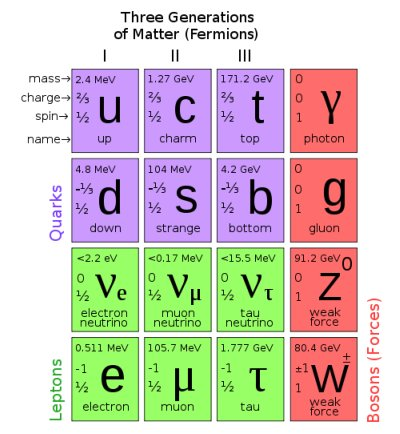
\includegraphics[width=0.45\textwidth]{Images/SM_zoo}
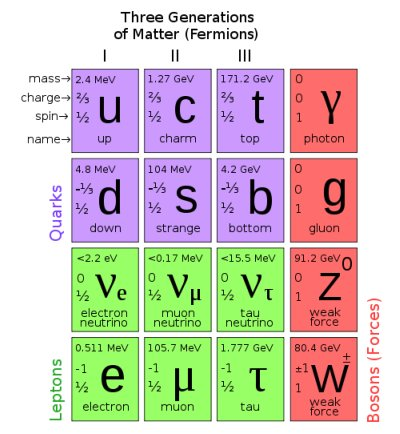
\includegraphics[width=0.45\textwidth]{Images/SM_zoo}
\caption{Elementary particles. }
\label{SM_zoo}
\end{figure}

\subsection{Gauge Symmetries}
\label{cap1:gaugeSymm}
The present belief is that all particles interactions may be dictated by the so called \textit{local gauge symmetries} and this is connected with the idea that  the conserved physical quantities (such as electric charge) are conserved in local regions of space and not just globally\cite{HalzenMartin}. \\
In particular, for the SM, the gauge group symmetry can be written as:
\[
SU(3)_{C}\otimes SU(2)_{L}\otimes U(1)_{Y}
\label{gaugeMS}
\]
where $SU(3)_{C}$ is the non-abelian group of strong interaction (QCD) and $SU(2)_{L}\otimes U(1)_{Y}$ is the group of the electroweak sector (EW) in which the electromagnetic and the weak force are described by one unified theory. As said, the SM is a local gauge theory and is it possible to associate a lagrangian obtained summing the contribution of the two gauge group:
\begin{equation}
\mathcal{L}_{MS} = \mathcal{L}_{EWK} + \mathcal{L}_{QCD}
\label{Lms}
\end{equation}

\begin{comment}
%The connection between symmetries and conservation laws is best discussed in the framework of Lagrangian Field Theory.\\
The fundamental quantity in classical mechanics is the action \textit{S}, the time integral of the Lagrangian \textit{L} (defined as the difference between the kinematic and potential energy):
\begin{equation}
S = \int L\, dt = \int \mathcal{L}(\phi, \partial \phi / \partial x_{\mu}) \,d^{4}x
\end{equation}
where $\mathcal{L}$ is the Lagrangian Density\footnote{however, following standard use in field theory, we will often refer to $\mathcal{L}$ simply Lagrangian.} 
and $\phi$ is the field, itself a function of the continuous parameters $x_{\mu}$ \cite{Peskin}\cite{Maggiore}. \\
Thanks to the \textit{Principle of least action}\footnote{Fixed the values of the coordinates at the initial and at the final time, classical trajectory which satisfies these conditions is an extremum of the action.} is possible deduce the particle equations of motion, the so called Euler-Lagrange equations (\ref{Eul_Lagr_Eq}):
\begin{equation}
\frac{\partial \mathcal{L}}{\partial \phi} - \frac{\partial}{\partial x_{\mu}}\frac{\partial \mathcal{L}}{\partial(\partial \phi / \partial x_{\mu})} = 0
\label{Eul_Lagr_Eq}
\end{equation}
%The relationship between symmetries and conservation laws is summarized in \textit{Noether's theorem}: 
\end{comment}

\subsubsection{QED}\index{QED}\label{QED}
%Quantum electrodynamics (QED) describes the interactions between photons and electrons. 
Starting point of the electroweak theory, is the  Quantum Electrodynamics, where is described the interaction of electron with photon.\\
Let's start with a complex field $\psi$ describing a free electron with mass m: its Lagrangian is
%Its motion is described by the Dirac Equation that follow from
% while the Dirac equation describes its motion. It can be shown Dirac equation follows from
\begin{equation}
\mathcal{L} = \bar{\psi}(i\gamma^{\mu}\partial_{\mu}-m)\psi
\label{L_electron}
\end{equation}
and its equation of motion can be deduced by the Dirac Equation.\\%, obtained substituting \ref{L_electron} in \ref{Eul_Lagr_Eq}. \\
The electromagnetic (em)  field instead is described by the four-vector gauge potential $A_{\mu}$. The field strength tensor is defined as:
\begin{equation}
F_{\mu\nu} = \partial_{\mu}A_{\nu} - \partial_{\nu}A_{\mu}
\label{F_em}
\end{equation}
and the equation of motion, in presence of an external current $J^{\mu}$ is:
\begin{equation}
\partial_{\mu}F^{\mu\nu} = QeJ^{\nu}
\label{Motion_em}
\end{equation}
In case now the electron interacts with the em field, the new Lagrangian is:
\begin{equation}
\mathcal{L}_{EM} = \bar{\psi}(i\gamma^{\mu}D_{\mu}-m)\psi - \frac{1}{4}F_{\mu\nu}F^{\mu\nu}
\label{L_electron_em}
\end{equation}
where $D_{\mu}$, known as covariant derivative, is defined as
\begin{equation}
D_{\mu} = \partial_{\mu} + ieQA_{\mu}
\label{D_covariante}
\end{equation}
and the last term in \ref{L_electron_em} stands for Maxwell's equation. \\
It can be shown that \ref{L_electron_em} is invariant under the phase transformation:
\begin{equation}
\psi(x)\to e^{-iQ\theta} \psi(x)
\label{global_trans}
\end{equation}
with $\theta \in \Re$. This transformation belongs to the group U(1) and according to Noether's theorem, it implies the existence of a conserved quantity: in this case, the electric charge.
Since once the value of $\theta$ is fixed, the invariance is specified for all space and time, it is known as \textit{global gauge invariance}. \\
More interesting is the case in which the parameter $\theta$ depends on space and time in a completely arbitrary way:
\begin{equation}
\psi(x)\to e^{-iQ\theta(x)} \psi(x)
\label{local_trans}
\end{equation}
and the Lagrangian \ref{L_electron_em} is not invariant.
It can be shown that, in oder to restore the Lagrangian invariance, the potential $A_{\mu}$ must satisfy following condition:
\begin{equation}
A_{\mu} \to A_{\mu} + \frac{1}{e}\partial_{\mu}\theta
\label{A_trans}
\end{equation}
Under \ref{local_trans} and \ref{A_trans} the Lagrangian \ref{L_electron_em} is invariant.\\ 
One can observe the absence of mass term in the Lagrangian: this means that the boson associated to the potential $A_{\mu}$, the photon, must be massless: the presence of a mass term would make the Lagrangian not invariant under gauge transformation. \\

\subsubsection{QCD}\index{QCD}\label{QCD}
The interaction between quarks and gluons is described by the Quantum Chromodynamics. \\
For quarks \cite{QCD}, it must be considered a new quantum number, the colour, such that each species of quark may have three different colours: $q_{j,\ j = 1, 2, 3}$ (red, green, blue). In order to avoid the existence of non-observed extra states with non-zero colour, one needs to further postulate that all asymptotic states are colourless, i.e. singlets under rotations in colour space. This assumption is known as the confinement hypothesis, because it implies the non-observability of free quarks: since quarks carry colour they are confined within colour-singlet bound states. \\
For free quark described by the field $q_{j}$, the Lagrangian is:
\begin{equation}
\mathcal{L} = \bar{q_{j}}(i\gamma^{\mu}\partial_{\mu} - m)q_{j}
\label{L_quark}
\end{equation}
In order to describe the  interaction between quarks and gluons, it is needed to change the quark derivative by covariant objects. Since there are now eight independent gauge parameters, eight different gauge bosons $G^{\mu}_{a}(x)$, the so-called gluons, are needed:
\begin{equation}
D^{\mu}_{q_{j}} \equiv [\partial^{\mu}- ig_{s}\frac{\lambda^{a}}{2}G^{\mu}_{a}(x)]
\label{D_covariante_qcd}
\end{equation}
The corresponding field strengths are also introduced:
\begin{equation}
G^{\mu\nu}_{a} = \partial^{\mu}G^{\nu}_{a} - \partial^{\nu}G^{\mu}_{a} + g_{s}f^{abc}G^{\mu}_{b}G^{\nu}_{c}
\label{G_munu}
\end{equation}
where $g_{s}$ is the coupling constant.
Hence, in case of interaction the new Lagrangian is:
\begin{equation}
\mathcal{L}_{QCD} = \bar{q_{j}}(i\gamma^{\mu}D_{\mu} - m)q_{j} -\frac{1}{4}G^{\mu\nu}_{a}G^{a}_{\mu\nu}
\label{L_quark_gluon}
\end{equation}
It can be shown \ref{L_quark_gluon} is invariant under arbitrary global $SU(3)_{C}$ transformations in colour space \ref{q_tranf_global}:
\begin{equation}
q(x) \to q'(x) = Uq(x) \equiv e^{i\theta_{a}T^{a}}q(x), \quad a = 1, 2, ...,8
\label{q_tranf_global}
\end{equation}
where $T_{a}$ are the generators of the SU(3) (a = $N^{2} - 1 = 3^{2} - 1 = 8)$ group linked with the $\lambda_{a}$ Gell-Mann matrices. \\
More interesting is the case in which $\theta$ depends on local coordinates, $\theta_{a}$ = $\theta_{a}$(x):
\begin{equation}
q(x) \to q'(x) = Uq(x) \equiv e^{i\theta_{a}(x)\frac{\lambda^{a}}{2}}q(x), \quad a = 1, 2, ...,8
\label{q_tranf_local}
\end{equation}
The group is non-Abelian since not all the generators $\lambda_{a}$ commute with each other. \\
To ensure the invariance of the Lagrangian \ref{L_quark_gluon}, the gauge fields must transform as follow:
\begin{equation}
G_{\mu a} \to G_{\mu a} - \frac{1}{g_{s}} \partial_{\mu}\theta_{a} - f_{abc}\theta^{b}G^{c}_{\mu}
\label{G_tranf_local}
\end{equation}
The field tensor $G^{\mu\nu}_{a}$ has a remarkable new property: imposing gauge symmetry (\ref{q_tranf_local} and \ref{G_tranf_local}), it has required kinematic energy term in \ref{L_quark_gluon} is not purely kinetic but includes an induced self-interaction between the gauge bosons. Decomposing the Lagrangian into its different pieces, there are three terms analogues to QED describing the free propagation of quarks and gluons and the quark-gluon interaction and two terms showing the presence of three and four gluon self-coupling in QCD reflecting the fact that gluons themselves carry color charge. They have no analogue in QED and arise on account of the non-Abelian character of the gauge group. As in QED, the absence of a mass term implies gluons must be massless.\\

\subsubsection{The electroweak theory}\index{EWK}
Low-energy experiments have provided a large amount of information about the dynamics underlying flavour-changing processes. The detailed analysis of the energy and angular distributions in $\beta$ decays, such as $\mu^{-} \to e^{-}\bar{\nu}_{e}\nu_{\mu}$, made clear that only the left-handed (right-handed) fermion (antifermion) chiralities participate in those weak transitions. Moreover, the strength of the interaction appears to be universal. \\
Using gauge invariance, it is possible to determine the right QED (\ref{L_electron_em}) and QCD (\ref{L_quark_gluon}) Lagrangians. To describe weak interactions, a more elaborated structure is needed, with several fermionic flavours and different properties for left- and right-handed fields. Moreover, the left-handed fermions should appear in doublets, and it would like to have gauge bosons in addition to the photon. The simplest group with doublet representations is SU(2) while to include also the electromagnetic interactions an additional U(1) group is needed. The obvious symmetry group to consider is then:
\begin{equation}
G \equiv SU(2)_{L} \otimes U(1)_{Y}
\label{EWK_group}
\end{equation}
where L refers to left-handed fields and Y stands for the weak hypercharge. \\
Let's consider a single family of leptons:
\begin{equation}
%\chi_L	&= \begin{pmatrix}\nu_{\emph{l}} \\\emph{l}^-\end{pmatrix}_L
\chi_{L} =  {\nu_{l} \choose l^{-}}_{L}, \quad \psi_{R} = l^{-}_{R}
\label{EWK_Singlet_doublet_Leptons}
\end{equation}
or for quarks
\begin{equation}
%\chi_L	&= \begin{pmatrix}\nu_{\emph{l}} \\\emph{l}^-\end{pmatrix}_L
\chi_{L} =  {u \choose d}_{L} , \quad \psi_{R} = u_{R},\ or\ d_{R}
\label{EWK_Singlet_doublet_Leptons}
\end{equation}
As in QED and QCD case, starts with free Lagrangian:
\begin{equation}
\mathcal{L} = i\bar{\chi}_{L}\gamma^{\mu}\partial_{\mu}\chi_{L} + i\bar{\psi}_{R}\gamma^{\mu}\partial_{\mu}\psi_{R}
\label{L0_EWK}
\end{equation}
The interaction is again introduced changing the derivative with the covariante:
\begin{equation}
D_{\mu} = \partial_{\mu} + igW_{\mu}^{a}T_{a} + ig'B_{\mu}Y
\label{D_EWK}
\end{equation}
where $W_{\mu}^{a}$ a = 1, 2, 3 are the three gauge bosons associated with the group $SU(2)_{L}$, $T^{a}$ its generators and g the coupling constants; $B_{\mu}$, Y and g are instead respectively the gauge boson, the generator and the coupling constant for the group $U(1)_{Y}$.
With $W_{\mu}^{a}$ and $B_{\mu}$ can be introduced also the tensor strength fields:
\begin{equation}
\begin{split}
W^{\mu\nu}_{a} &= \partial^{\mu}W^{\nu}_{a} - \partial^{\nu}W^{\mu}_{a} + g\epsilon^{abc}W^{\mu}_{b}W^{\nu}_{c} \\
B^{\mu\nu} 	 &= \partial^{\mu}B^{\nu} - \partial^{\nu}B^{\mu}
\label{WB_munu}
\end{split}
\end{equation}
Therefore, the properly Lagrangian is given by:
\begin{equation}
\mathcal{L} = i\bar{\chi}_{L}\gamma^{\mu}D_{\mu}\chi_{L} + i\bar{\psi}_{R}\gamma^{\mu}D_{\mu}\psi_{R} - \frac{1}{4}B_{\mu\nu}B^{\mu\nu} - \frac{1}{4}W_{\mu\nu}W^{\mu\nu}
\label{L_EWK}
\end{equation}
In \ref{L_EWK} $W_{\mu\nu} = W^{a}_{\mu\nu}\sigma^{a}/2$ with $\sigma^{a}$ 2x2 Pauli's matries. \\
As in QED and QCD case, also electroweak interaction is invariant under global transformation:
\begin{equation}
\begin{split}
\chi_{L} \to \chi_{L}' &= e^{i\alpha_{a} T^{a}  + i\beta Y} \chi_{L} \\
\psi_{R} \to \psi_{R}' &= e^{i\beta Y} \psi_{R} \\
\label{EWK_global}
\end{split}
\end{equation}
Moving to local transformation, in order to guarantee Lagrangian \ref{L_EWK} to be invariant, the gauge bosons must have following transformation rules:
\begin{equation}
\begin{split}
W^{a}_{\mu} &\to U_{L}(x) W^{a}_{\mu}  U_{L}(x)^{\dagger} - \frac{i}{g}\partial_{\mu}U_{L}(x) U_{L}(x)^{\dagger}, \\
B_{\mu} &\to B_{\mu} + \frac{1}{g'}\partial_{\mu}\beta
\label{EWK_global}
\end{split}
\end{equation}
where $U(x)_{L} = e^{i\sigma_{a} / 2\ \alpha(x)^{a}}$. The transformation of $B_{\mu}$ is identical to the one obtained in QED for the photon, while the $SU(2)_{L}\ W^{a}_{\mu}$ fields transform in analogous way to the gluon fields of QCD. \\
The gauge symmetry forbids to write a mass term for the gauge bosons in \ref{L_EWK}. Fermionic masses are also not possible, because they would communicate the left- and right-handed fields, which have different transformation properties, and therefore would produce an explicit breaking of the gauge symmetry. Thus, the $SU(2)_{L} \otimes U(1)_{Y}$ Lagrangian in \ref{L_EWK} only contains massless fields.\\
The term containing the $SU(2)_{L}$ matrix:
\begin{equation}
\frac{\sigma_{a}}{2}W_{\mu}^{a} = \frac{1}{\sqrt{2}}\begin{pmatrix} \sqrt{2}W^{3}_{\mu} & W_{\mu}^{+} \\ W_{\mu}^{-} & - \sqrt{2}W^{3}_{\mu} \end{pmatrix}
\end{equation}
gives rise to charged-current interactions with the bosons field $W_{\mu}^{\pm} \equiv (W^{1}_{\mu} \mp iW^{2}_{\mu}) / \sqrt{2}$. \\
La Lagrangian \ref{L_EWK}  contains also interactions with the neutral gauge field $W^{3}_{\mu}$ and $B_{\mu}$; one can define
\begin{equation}
Z_{\mu} = \frac{gW^{3}_{\mu} - g'B_{\mu}}	{\sqrt{g^{2}+g'{2}}}, \quad A_{\mu} = \frac{gW^{3}_{\mu} + g'B_{\mu}}	{\sqrt{g^{2}+g'{2}}}
\label{A_Z}
\end{equation}
and thinking them as a rotation, introducing the Weinberg angle $\theta_{W}$ so that $\cos\theta_{W} = g/{\sqrt{g^{2}+g'{2}}}$ (and $\sin\theta_{W} = g'/{\sqrt{g^{2}+g'{2}}}$):
\begin{equation}
Z_{\mu} = \cos\theta_{W}W^{3}_{\mu} - \sin\theta_{W}B_{\mu}, \quad A_{\mu} = \sin\theta_{W}W^{3}_{\mu} + \cos\theta_{W}B_{\mu}
\label{A_Z_2}
\end{equation}
or reversing:
\begin{equation}
{W^{3}_{\mu} \choose B_{\mu}} \equiv \begin{pmatrix} \cos\theta_{W} & \sin\theta_{W} \\ -\sin\theta_{W} & \cos\theta_{W} \end{pmatrix} {Z_{\mu} \choose A_{\mu}}
\label{W_B_A_Z}
\end{equation}
With these definitions, it can be observed the $A_{\mu}$ in \ref{L_EWK} couples in the same way with $l_{L}$ and $l_{R}$ as the photon: to get QED from these one needs to impose
\begin{equation}
g\sin\theta_{W} = g'\cos\theta_{W} = e
\label{g_gprime}
\end{equation}
At the same time, $Z_{\mu}$, can be identify with the Z boson, mediator of the Weak Interaction. \\
Once again, no mass term is present in \ref{L_EWK} and this means that $W^{\pm}$ and Z must be massless: this is in contrast with experimental evidence \cite{Wboson}\cite{Zboson}. \\
The way to generate the mass of the particle is through the so called \textit{Spontaneous Symmetry Breaking} (SSB): this mechanism appear in those cases where one has a symmetric Lagrangian, but a non-symmetric vacuum. 

\subsection{Spontaneous Symmetry Breaking: SSB}
Let's consider a complex scalar field $\phi(x) = (\phi_{1} + \phi_{2}) / \sqrt{2}$, with Lagrangian:
\begin{equation}
\mathcal{L} \equiv T - V = (\partial_{\mu}\phi)^{*}(\partial^{\mu}\phi) - \mu^{2}(\phi^{*}\phi)-\lambda(\phi^{*}\phi)^{2}
\label{L0}
\end{equation}
\ref{L0} is invariant under global phase transformation of the scalar field (it possesses a U(1) global gauge symmetry). \\
Considering the case when $\lambda > 0$, for the quadratic piece there are two possibilities:
\begin{itemize}
\item{$\mu^{2} > 0$:} the potential has only the trivial minimum $\phi = 0$
\item{$\mu^{2} < 0$:} the minimum is every point belonging to the circle (in the $\phi_{1}, \phi_{2}$) of radius $\nu$ such that:
	\begin{equation}
	(\phi_{1})^{2}+(\phi_{2})^{2} = \nu^{2} \quad with\ \nu^{2} = - \frac{\mu^{2}}{\lambda}
	\end{equation}
	as shown in \figurename~\ref{V_phi_potential}
\end{itemize}
\begin{figure}[htbp]
\centering
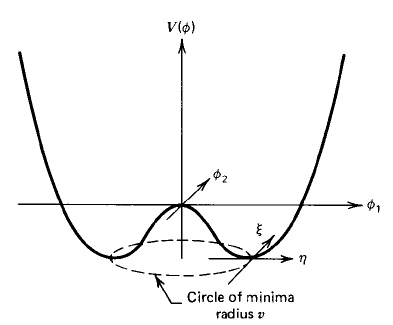
\includegraphics[width=0.45\textwidth]{Images/Vphi.png}
\caption{The potential $V(\phi)$ for a complex scalar field with $\lambda > 0$ and $\mu^{2} < 0$. }
\label{V_phi_potential}
\end{figure}
Owing to the U(1) phase-invariance of the Lagrangian \ref{L0}, there is an infinite number of degenerate states of minimum energy. 
By choosing a particular solution, $\phi_{1} = \nu$ and $\phi_{2} = 0$, as the ground state, the symmetry gets spontaneously broken. Parametrising the excitations over the ground state as:
\begin{equation}
\phi(x) \equiv \frac{1}{\sqrt{2}}[\nu+\eta(x)+i\xi(x)]
\label{phi_expansion}
\end{equation}
and substituting into \ref{L0}, one obtains:
\begin{equation}
\mathcal{L'} = \frac{1}{2}(\partial_{\mu}\xi)^{2} + \frac{1}{2}(\partial_{\mu}\eta)^{2} + \mu^{2}\eta^{2} + const. + O(\eta^{3})+O(\xi^{3})
\label{L0_prime}
\end{equation}
The third term has the form of a mass term for $\eta$-field: the $\eta$-mass is $m_{\eta} = \sqrt{-2\mu^{2}}$. The first term in \ref{L0_prime} represents the kinetic energy of the $\xi$-field but there is no corresponding mass term for the $\xi$. The fact there are massless excitations associated with the SSB mechanism is completely general result, known as the \textit{Goldstone theorem}: if a Lagrangian is invariant under a continuous symmetry group G, but the vacuum is only invariant under a subgroup $H\subset G$, then there must exist as many massless spin-0 particles (Goldstone bosons) as broken generators (i.e., generators of G which do not belong to H).

\subsubsection{Brout-Englert-Higgs mechanism}%: U(1) local gauge symmetry}
Let's move to consider the case for spontaneous breaking of U(1) local gauge symmetry.\\
Taking into account the covariant derivative \ref{D_covariante} where the gauge filed transforms as in \ref{A_trans}, the new Lagrangian can be written as
\begin{equation}
\mathcal{L} = D^{\mu}\phi^{*}D_{\mu}\phi -\mu^{2}\phi^{*}\phi-\lambda(\phi^{*}\phi)^{2}-\frac{1}{4}F_{\mu\nu}F^{\mu\nu}
\label{L0_U1}
\end{equation}
If $\mu^{2} > 0$, \ref{L0_U1} is just the QED Lagrangian for a charged scalar particle of mass $\mu$.
For the case $\mu^{2} < 0$, it is interesting to note that to lowest order in $\xi$, \ref{phi_expansion} can be expressed as
\begin{equation}
\phi(x) \equiv \frac{1}{\sqrt{2}}[\nu+\eta(x)]e^{i\xi(x)/\nu}
\label{phi_expansion_2}
\end{equation}
and this suggests to use different set of real field: h, $\theta$, $A_{\mu}$ where now
\begin{equation}
\begin{split}
\phi(x) &\to \frac{1}{\sqrt{2}}[\nu+h(x)]e^{i\theta(x)/\nu}, \\
A_{\mu} &\to A_{\mu}+ \frac{1}{e\nu}\partial_{\mu}\theta
\end{split}
\label{new_phi_A}
\end{equation}
This is a particular choice of gauge, with $\theta(x)$ chosen so that h is real. Substituting \ref{new_phi_A} in \ref{L0_U1}, one obtains:
\begin{equation}
\begin{split}
\mathcal{L}' = &\frac{1}{2}(\partial_{\mu}h)^{2}-\lambda\nu^{2}h^{2}+\frac{1}{2}e^{2}\nu^{2}A_{\mu}^{2}-\lambda\nu h^{3}-\frac{1}{4}\lambda h^{4}\\
&+\frac{1}{2}e^{2}A_{\mu}^{2}h^{2}+\nu e^{2}A_{\mu}^{2}h-\frac{1}{4}F_{\mu\nu}F^{\mu\nu}
\end{split}
\label{L0_U1_prime}
\end{equation}
The Goldstone boson does not appear in the theory: this is because it corresponds only to the degree of freedom to make a gauge transformation. The Lagrangian \ref{L0_U1_prime} describes just two interacting massive particles, a vector gauge bosoon $A_{\mu}$ and a massive scalar h, which is called a \textit{Higgs particle}. 
%This is called the \textit{Higgs mechanism}.\\
%\subsubsection{The Higgs Mechanism for $SU(2)_{L} \otimes U(1)_{Y}$ symmetry
Consider now the case of  $SU(2)_{L} \otimes U(1)_{Y}$ symmetry \cite{SU2_Hmechanism} with the Lagrangian
\begin{equation}
\mathcal{L} = (D_{\mu}\phi)^{\dagger}(D^{\mu}\phi)-\mu^{2}\phi^{\dagger}\phi-\lambda(\phi^{\dagger}\phi)^{2}
\label{L0_SU2}
\end{equation}
$D_{\mu}$ is the covariant derivative \ref{D_EWK} and $\phi$ is an SU(2) doublet of complex scalar fields:
\begin{equation}
\phi(x) \equiv {\phi^{+}(x) \choose \phi^0(x)}
\label{phi_SU2}
\end{equation}
\ref{L0_SU2} is invariant under local $SU(2)_{L} \otimes U(1)_{Y}$ transformations. \\
In $\mu^{2} < 0$ and $\lambda^{2} > 0$ conditions, to generate gauge boson masses, a vacuum expectation value of $\phi(x)$ must be chosen:
\begin{equation}
\phi_{0} \equiv \frac{1}{\sqrt{2}}{0 \choose \nu}
\label{SU2_U1_V0}
\end{equation}
In this way, the symmetry is broken and this generates a mass for the corresponding gauge boson. This particular choice of $\phi_{0}$ breaks both $SU(2)$ and $U(1)_{Y}$ gauge symmetries but since it is neutral, the $U(1)_{em}$ remains unbroken and this means the photon remains massless. \\
Now, substituting the vacuum expectation value $\phi_{0}$ for $\phi(x)$ in the Lagrangian \ref{L0_SU2}, the expression for W and Z bosons mass are:
\begin{equation}
M_{W}^{2} = \frac{\nu^{2}g^{2}}{4}, \quad M_{Z}^{2} = \frac{\nu^{2}g^{2}}{4\cos^{2}\theta_{W}}=\frac{M_{W}^{2}}{\cos^{2}{\theta_{W}}}
\label{WZ_mass_expression}
\end{equation}
From experimental observation \cite{PDG}:
\begin{equation}
M_{Z} = 91.1876\pm0.0021\ GeV, \quad M_{W} = 80.385\pm 0.015\ GeV
\end{equation}
From these experimental numbers, one obtains the electroweak mixing angle:
\begin{equation}
\sin^{2}\theta_{W} = 1-\frac{M^{2}_{W}}{M^{2}_{Z}} = 0.22336 \pm 0.00010
\end{equation}
The scalar vacuum expectation value is:
\begin{equation}
\nu=(\sqrt{2}G_{F})^{-1/2}=246\ GeV
\end{equation}
where $G_{F} = 1.1663787 \times 10^{-5} GeV^{-1}$ is the Fermi coupling whose value can be measured with the muon lifetime \cite{muLifetime}.\\
From \ref{L0_SU2}, the potential $V(\phi)$ can be seen as:
\begin{equation}
V(\phi)=-\frac{1}{4}\lambda\nu^{2}+V_{H}+V_{HG^{2}}
\label{V0_Higgs}
\end{equation}
The first term stands for mass of the new Higgs boson: $m_{H} = \sqrt{2\lambda\nu^{2}}$; the second represents Higgs boson self-interaction and the last the coupling with the weak bosons (W and Z). \\
It is interesting to note the same Higgs doublet which generates weak bosons masses can give masses also to leptons and quarks. \\
In particular, let's consider the following Lagrangian:
\begin{equation}
\mathcal{L} = -G_{e} [(\bar{\nu}_{e},\ \bar{e})_{L}{\phi^{+} \choose \phi^{0}}e_{R}+\bar{e}_{R}(\phi^{-},\ \bar{\phi}^{0}){\nu_{e} \choose e}_{L} ]
\label{L0_fermion_quark_mass}
\end{equation}
Substituting the expression of $\phi$:
\begin{equation}
\phi = \frac{1}{\sqrt{2}}{0 \choose \nu+h(x)}
\end{equation}
into \ref{L0_fermion_quark_mass}, the Lagrangian becomes:
\begin{equation}
\mathcal{L} = -\frac{G_{e}}{\sqrt{2}}\nu(\bar{e}_{L}e_{R}+\bar{e}_{R}e_{L})-\frac{G_{e}}{\sqrt{2}}h(\bar{e}_{L}e_{R}+\bar{e}_{R}e_{L})
% [(\bar{\nu}_{e},\ \bar{e})_{L}{\phi^{+} \choose \phi^{0}}e_{R}+\bar{e}_{R}(\phi^{-},\ \bar{\phi}^{0}){\nu_{e} \choose e}_{L} ]
\label{L0_fermion_quark_mass_2}
\end{equation}
Choosing $G_{e}$ so that $m_{e} = G_{e}\nu/\sqrt{2}$, since the $G_{e}$ is arbitrary, the actual mass of the electron is not predicted. \\
The quark masses are generated in the same way with the difference that to generate a mass for the upper member of a quark doublet, a new Higgs doublet from $\phi$ must be used:
\begin{equation}
\phi_{c} = i\tau\phi^{*}={-\bar{\phi}^{0} \choose \phi^{-}} \xrightarrow[breaking]{}\frac{1}{\sqrt{2}}{\nu+h(x) \choose 0}
\end{equation}
The new Lagrangian can be written as:
\begin{equation}
\mathcal{L}= -G_{d}(\bar{u}, \ \bar{d})_{L}{\phi^{+} \choose \phi^{0}}d_{R}-G_{u}(\bar{u}, \ \bar{d})_{L}{-\bar{\phi}^{0} \choose \phi^{-}}u_{R}\ +\ hermitian\  coniugate
\label{L0_quark_mass}
\end{equation}
In \ref{L0_quark_mass}, the (u,\ d) quark doublet are considered even if the weak interactions operate on $(u,\  d')_{L}$ where the primed states are  linear combinations of the flavour eigenstates\footnote{Linear combination of the flavour eigenstates considering Cabibbo-Kobayashi-Maswaka (CKM) matrix: $d'_i = \sum_{n=1}^NV_{in}d_n  $ where N = 3 is the number of quarks, $V_{in}$ is CKM matrix and $d_{n}$ are the d type quarks d, s, b.}. Using these new doublets, \ref{L0_quark_mass} is therefore of the form:
\begin{equation}
\mathcal{L}= -G_{d}^{ij}(\bar{u}, \ \bar{d}')_{L}{\phi^{+} \choose \phi^{0}}d_{jR}-G_{u}^{ij}(\bar{u}, \ \bar{d}')_{L}{-\bar{\phi}^{0} \choose \phi^{-}}u_{jR}\ +\ hermitian\  coniugate
\label{L0_quark_mass_2}
\end{equation}
with i, j = 1, ..., N,  where N is the number of quark doublet. Substituting $\phi_{c}$ expression, the masses depend on the arbitrary couplings $G_{u,d}$ but, as for electron, it cannot be predicted.\\
The choose of a particular single Higgs doublet is sufficient on one hand to generate the masses of both the gauge bosons and the fermions but on the other hand, the masses of the fermoins are just parameteres of the theory and are not predicted. 
%At the same time, the mass of the Higgs $m_{h}$ is itself not predicted: from the first two terms of the effective potential, $V(\phi) = \mu^{2}\phi^{\dagger}\phi+\lambda(\phi^{\dagger}\phi)^{2}+O(3)$, the mass can be defined as $m_{h}^{2} = 2\nu^{2}\lambda$: theoretical limits indicate that $m_{h} \ge 10\ GeV$. \\
\\ To summarise, the complete Lagrangian of the SM is:
\begin{equation}
\begin{split}
\mathcal{L}_{SM} &= \frac{1}{4}W_{\mu\nu}\cdot W^{\mu\nu} - \frac{1}{4}B_{\mu\nu}B^{\mu\nu} + \bar{L}\gamma^{\mu}(i\partial_{\mu}-g\frac{1}{2}\tau \cdot W_{\mu} -g'\frac{Y}{2}B_{\mu})L \\
&+\bar{R}\gamma^{\mu}(i\partial_{\mu}-g'\frac{Y}{2}B_{\mu})R+|i\partial_{\mu}-g\frac{1}{2}\tau \cdot W_{\mu} -g'\frac{Y}{2}B_{\mu}|^{2} -V{\phi} \\
&-(G_{1}\bar{L}\phi R+G_{2}\bar{L} \phi_{c}R +\ hermitian\ conjugate)
\label{L0_SM}
\end{split}
\end{equation}
The first two terms represent the $W^{\pm}$, Z, $\gamma$ kinetic energies and the self-interactions; the third and the fourth term the lepton and quark kinetic energies and their interaction with weak W, Z and $\gamma$; the last terms stand for masses and coupling of the Higgs, bosons, leptons and quark. \\
Without the Higgs boson, the calculability of the SM would have been spoiled. In particular, perturbative unitarity \cite{PerturbativeHiggs_1, PerturbativeHiggs_2} would be lost at high energies as the longitudinal W/Z boson scattering amplitude would grow as the centre-of-mass energy increases. Moreover, the radiative corrections to the gauge boson self-energies would exhibit dangerous logarithmic divergences that would be difficult to reconcile with Electroweak precision data. With the discovery of the Higgs boson, it has been experimentally established that the SM is based on a gauge theory that could a priori be consistently extrapolated to the Planck scale.

\section{The Higgs boson}
The SM Higgs boson is a CP-even scalar of spin 0 \cite{PDG}. Its mass is given by $m_{h} = \sqrt{2\lambda\nu^{2}}$, where $\lambda$ is the Higgs self-coupling parameter in the potential $V(\phi)$. The experimentally Higgs mass, $m_{h} \simeq 125\ GeV$ \cite{ALTAS_H, CMS_H}, implies $\lambda \simeq 0.1$. 
%Once the mass is know, in the SM, the boson width is very precisely predicted: for a mass of 125 GeV, the Higgs boson has a very narrow width of 4.2MeV.
The Higgs boson couplings to the fundamental particles are set by their masses: very weak for light particles, such as up and down quarks, and electrons, but strong for heavy particles such as the W and Z bosons and the top quark. In particular, the SM Higgs coupling to fundamental fermions are linearly proportional to the fermion masses $m_{f}$ ($y_{f} = m_{f}/\nu$ where $y_{f}$ is the Yukawa coupling) whereas the couplings to bosons are proportional to the squares of the boson masses. As consequence, the dominant mechanism for Higgs boson production and decay involve the coupling of H to W, Z and/or the third generation quarks and leptons. The Higgs boson coupling to  gluons is induced at leading order by a one-loop process in which H couples to a virtual $t\bar{t}$ pair. Likewise, the Higgs boson couplings to photons is also generated via loops, although in this case the one-loop graph with a virtual $W^{+}W^{-}$ pair provides the dominant contribution and the one involving a virtual $t\bar{t}$ pair is subdominant. \\

\subsection{The Higgs boson: production mechanisms}
The main production mechanisms at the LHC are gluon fusion, weak-boson fusion, associated production with gauge boson and associated production with a pair of top/antitop quarks. 
The corresponding Feynman diagrams are reported in \figurename~\ref{Feynman_H_production}; \figurename~\ref{plot_13tev_H_production} summarises the cross section as a function of Higgs mass for these dominant Higgs production processes for a center of mass energy of 13 TeV. 

\begin{figure}[htbp]
\centering
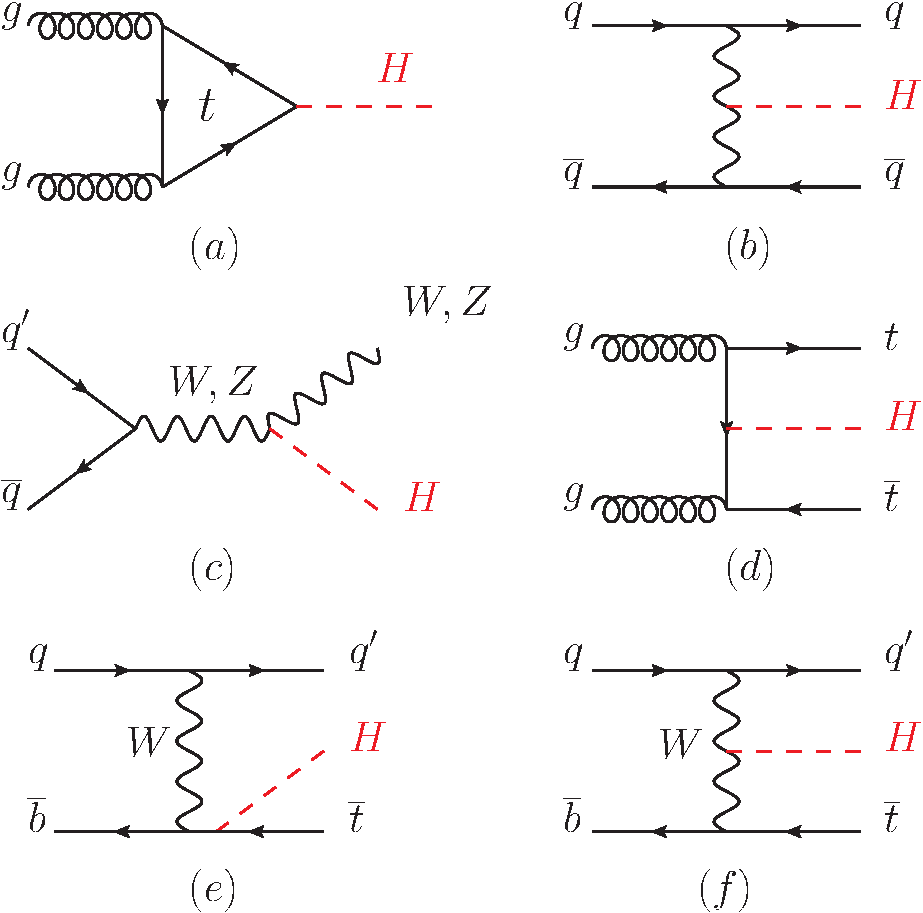
\includegraphics[width=0.45\textwidth]{Images/Feynman_H_production}
\caption{Main Leading Order Feynman diagrams contributing to the Higgs production: (a) gluon fusion, (b) Vector-boson fusion, (c) Higgs-strahlung (or associated production with a gauge boson), (d) associated production with a pair of top (or bottom quarks), (e-f) production in association with a single top quark.}
\label{Feynman_H_production}
\end{figure}
\begin{figure}[htbp]
\centering
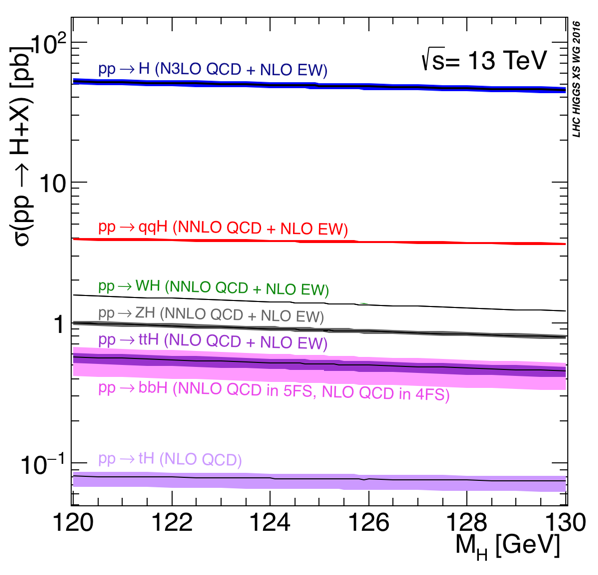
\includegraphics[width=0.45\textwidth]{Images/plot_13tev_H_production}
\caption{Standard Model Higgs boson production cross section at $\sqrt{s} = 13\ TeV$ as a function of Higgs boson mass \cite{HiggsTWiki}.}
\label{plot_13tev_H_production}
\end{figure}

\subsubsection{Production mechanism: gluon fusion}
The Higgs boson production mechanism with the largest cross section is the gluon-fusion process: $gg \to H + X$, mediated by the exchange of a virtual, heavy top quark (\figurename~\ref{Feynman_H_production}a). Contributions from lighter quarks propagating in the loop are suppressed proportional to $m_{q}^{2}$. QCD radiative corrections to this process are also very important. At the LHC, with a $\sqrt{s} = 13\ TeV$, the value for the production cross section at the next-to next- to next  to leading order is \cite{ggF_value}:
\begin{equation}
\sigma^{N3LO}_{ggF} = 48.6pb^{+2.2pb(+4.6\%)}_{-3.3pb(+6.7\%)}(theory) \pm 1.6(3.2\%)(PDF+\alpha_{s})
\label{ggH_cross_section}
\end{equation}

\subsubsection{Production mechanism: Weak-boson fusion}
The SM Higgs production mode with the second-largest cross section is Vector Boson Fusion (VBF): $qq \to qqH$ (\figurename~\ref{Feynman_H_production}b). This mechanism proceeds by the scattering of two (anti-)quarks, mediated by exchange of a W or Z boson, with the Higgs boson radiated off the weak-boson propagator. The scattered quarks give rise to two hard jets in the forward and backward regions of the detector. Gluon radiation in the central-rapidity is suppressed thanks to the color-singlet nature of the weak-gauge boson exchange: this feature let to distinguish VBF from overwhelming QCD backgrounds including gluon-fusion induced Higgs + 2 jets production and production of H in association with a W or Z boson hadronically decaying. This process receive contributions at NLO from QCD and EW; QCD also contributes at NNLO.

\subsubsection{Production mechanism: Higgs-strahlung}
The next most relevant Higgs boson production mechanism is the Higgs-strahlung, the production of the Higgs boson with W or Z gauge bosons: $pp \to VH + X$ with $V = W^{\pm},Z$ (\figurename~\ref{Feynman_H_production}c). As in VBF, at NLO EW and QCD (due to corrections to the Drell-Yan cross section) give their contributions to this cross section. In addition, Higgs-strahlung receives non Drell-Yan-like corrections in the $q\bar{q}$ channel where the Higgs is radiated off top-quarks loops.

\subsubsection{Production mechanism: $t\bar{t}H$}
Higgs radiation off top quarks (\figurename~\ref{Feynman_H_production}d), $pp \to t\bar{t}H$, provides a direct probe of the top-Higgs Yukawa coupling. On the 10th April 2018, CMS announced the observation of the production of the Higgs boson together with a top-quark pair \cite{ttH}. \figurename~\ref{ttH} shows a possible t$\bar{t}$H event.
\begin{figure}[htbp]
\centering
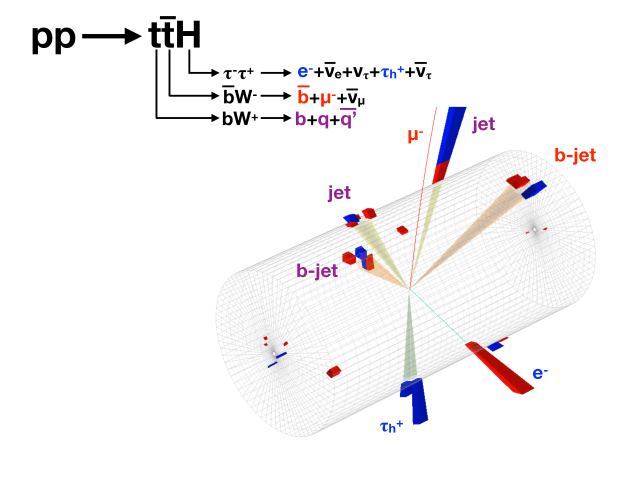
\includegraphics[width=0.45\textwidth]{Images/ttH}
\caption{An event candidate for the production of a top quark and top anti-quark pair in conjunction with a Higgs Boson in the CMS detector. The Higgs decays into a $\tau^+$ lepton and a $\tau^-$ lepton; the $\tau^+$ in turn decays into hadrons and the $\tau^-$ decays into an electron. The decay product symbols are in blue. The top quark decays into three jets (sprays of lighter particles) whose names are given in purple. One of these is initiated by a b-quark. The top anti-quark decays into a muon and b-jet, whose names appear in red \cite{ttH_event}.}
\label{ttH}
\end{figure}

\subsection{The Higgs boson: decay channels}
As reported in \figurename~\ref{Higgs_decay}, the dominant decay modes for the Higgs boson are $H \to b\bar{b}$, $H \to WW^{*}$ followed by $H \to \gamma \gamma$, $H \to \tau^{+}\tau^{-}$ and $H \to ZZ^{*}$;  \tablename~\ref{Higgs_decay_table} summarises the branching ratios and the relative uncertainty for these decay channels. As example, in \figurename~\ref{Higgs_decay} is reported the mass 4 leptons mass distribution comparing data and simulation.\\
Of particular interest is the dimuon decay channel: it has a small branching ratio ($2.18 \times 10^{-4}$) but it plays a fundamental role. This decay channel is the only way to directly measure the Higgs-muon Yukawa coupling strength and the comparison of the cross section of $H\to \mu\mu$ and $H\to \tau\tau$ could provide constraints on the proportionality of the Higgs couplings to fermions of different generations and of leptons with different masses. 
\begin{figure}[htbp]
\centering
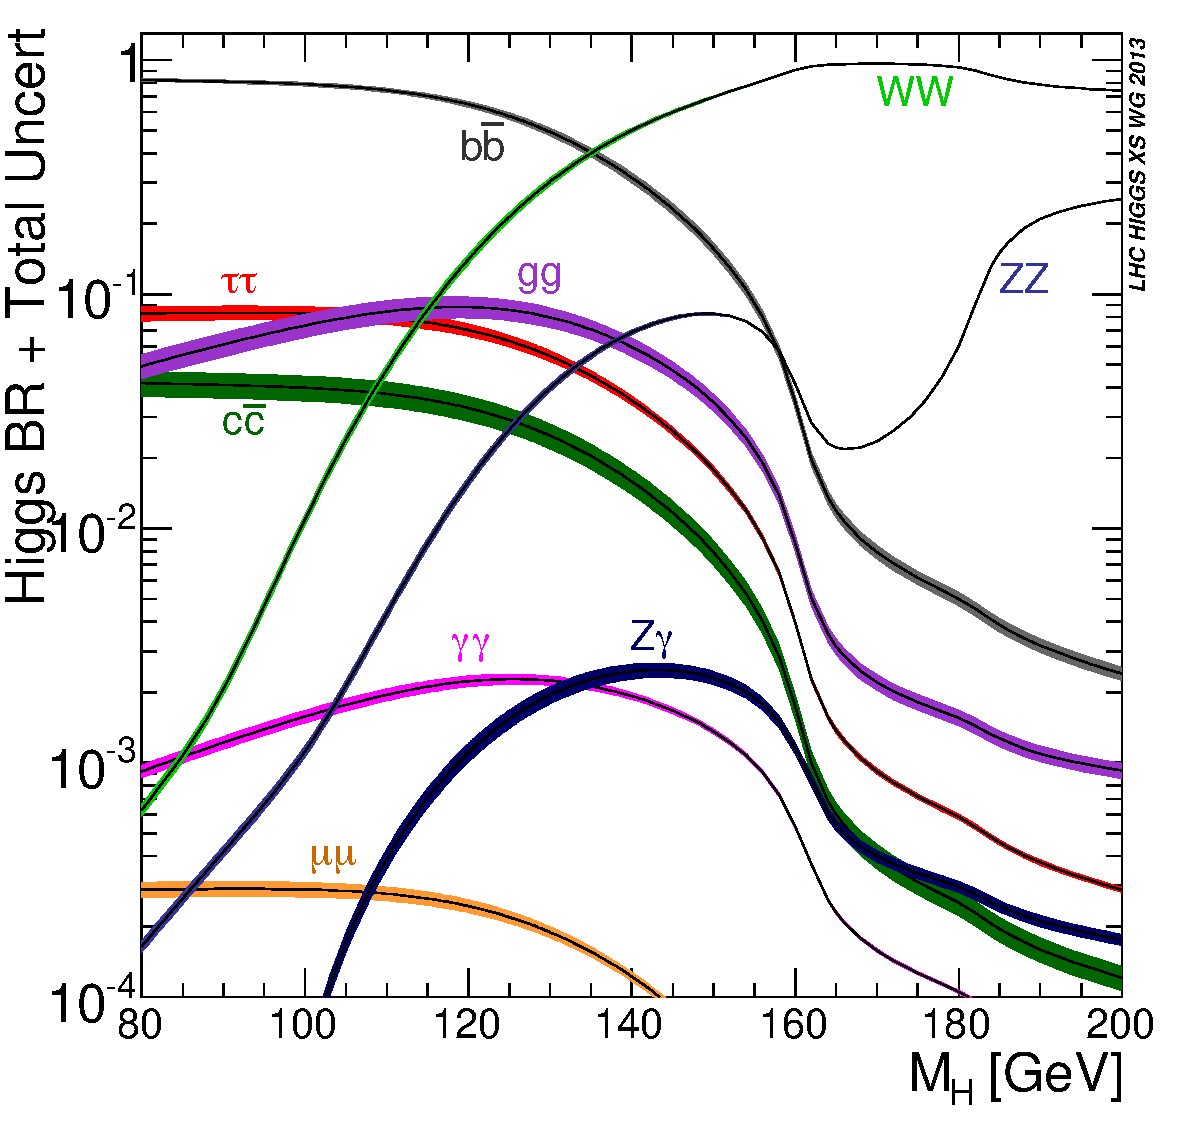
\includegraphics[width=0.45\textwidth]{Images/Higgs_decay}
\caption{Standard Model Higgs boson production cross section at $\sqrt{s} = 13\ TeV$ as a function of Higgs boson mass \cite{HiggsTWiki}.}
\label{Higgs_decay}
\end{figure}
\begin{table}[ht]	
	\begin{center}
		\begin{tabular}{ccc}
			\hline   Decay channel & Branching ratio  & Rel. uncertainty  \\
			\hline
			 \multirow{2}*{$H \to b\bar{b}$} & 			\multirow{2}*{$5.84 \times 10^{-1}$} &	 +3.2\% \\  &  & -3.3\% \\
			 \multirow{2}*{$H \to WW^{*}$} &			 \multirow{2}*{$2.14 \times 10^{-1}$} &	 +4.3\% \\  &  & -4.2\% \\
			 \multirow{2}*{$H \to \tau^{+}\tau^{-}$} &		 \multirow{2}*{$6.27 \times 10^{-2}$} &	 +5.7\% \\  &  & -5.7\% \\
			 \multirow{2}*{$H \to ZZ^{*}$} &				 \multirow{2}*{$2.62 \times 10^{-2}$} &	 +4.3\% \\  &  & -4.1\% \\
			 \multirow{2}*{$H \to \gamma \gamma$} & 	\multirow{2}*{$2.27 \times 10^{-3}$} &	 +5.0\% \\  &  & -4.9\% \\
			 \multirow{2}*{$H \to \mu \mu$} &			 \multirow{2}*{$2.18 \times 10^{-4}$} &	 +6.0\% \\  &  & -5.9\% \\
			\hline
		\end{tabular}
	\end{center}
	\caption{Branching ratio for a Higgs boson with $m_H$ = 125 GeV at 13 TeV \cite{BR_1, BR_2}.}
	\label{Higgs_decay_table}
\end{table}
\begin{figure}[htbp]
\centering
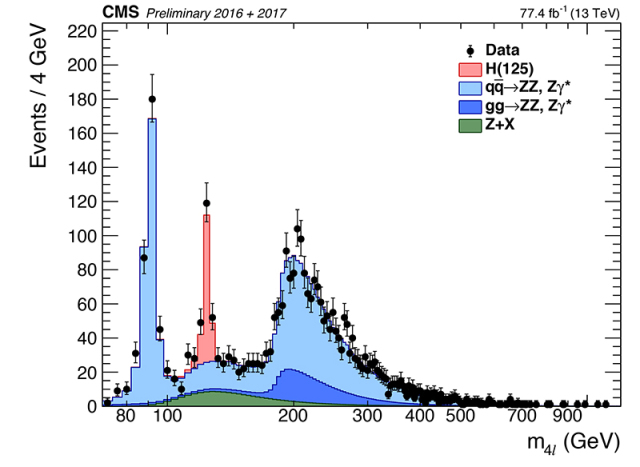
\includegraphics[width=0.5\textwidth]{Images/HZZ}
\caption{Distribution of the four-lepton reconstructed invariant mass $m_{4l}$ in the full mass range combining 2016 and 2017. Points with error bars represent the data and stacked histograms represent expected distributions of the signal and background processes \cite{HZZ_mass}}
\label{HZZ}
\end{figure}

\subsection{Latest Higgs results}
\subsubsection{Signal Strength}
In \figurename~\ref{SignalStrength} are reported the fit to the signal strength modifiers $\mu_i$: $\mu_i$ is defined as the ratio between the measured Higgs boson yield and its SM expectation. For a specific production and decay channel $i \to H \to f$ , the signal strengths for the production, $\mu_i$ , and for the decay, $\mu_f$ , are defined as,
\[
\mu_i = \frac{\sigma_i}{(\sigma_i)_{SM}},\ \ \ \mu^f = \frac{BR^f}{{BR}^f_{SM}}
\]
where $\sigma_i$ is the production cross section for $i \to H$ and $\mu^f$ is the the branching ratio for  $H \to f$; the "SM" refers to their respective SM predictions, so by definition, the SM corresponds to $\mu_i = \mu^f = 1$. Since $\sigma_i$ and $BR^f$ cannot be separately measured without additional assumptions, only the product of $\mu_i$ and $\mu^f $ can be extracted experimentally, leading to a signal strength $\mu^f_i$ for the combined production and decay:
\[
\mu^f_i = \frac{\sigma_i \cdot BR^f}{(\sigma_i)_{SM}\cdot {BR}^f_{SM}} = \mu_i \times \mu^f
\]
The combined measurement of the common signal strength modifier is \cite{LatestHiggsCMS}
\[
\mu = 1.17^{+0.06}_{-0.06}(stat.)^{+0.06}_{-0.05}(sig.th.)^{+0.06}_{-0.06}(other\ syst.) 
\]
\begin{figure}[htbp]
\centering
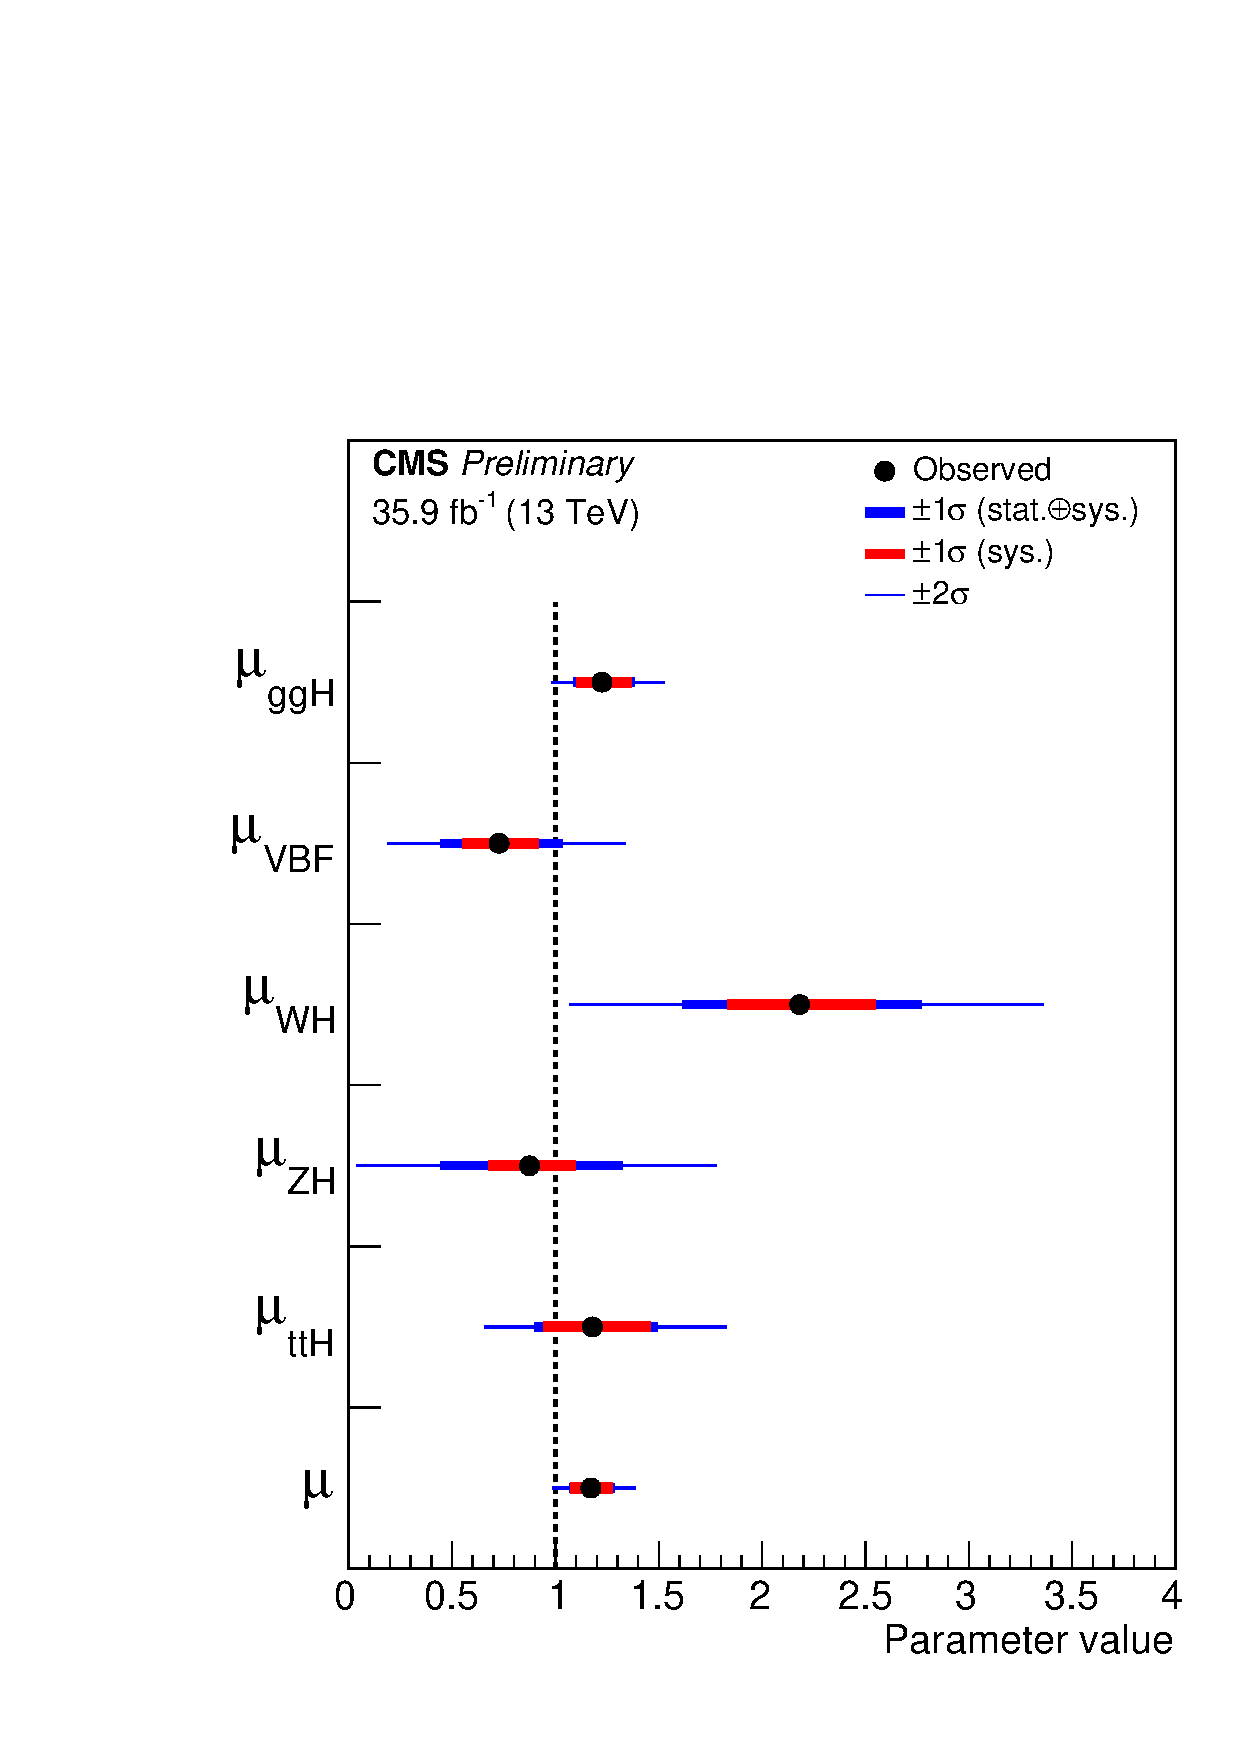
\includegraphics[width=0.45\textwidth]{Images/MuI}
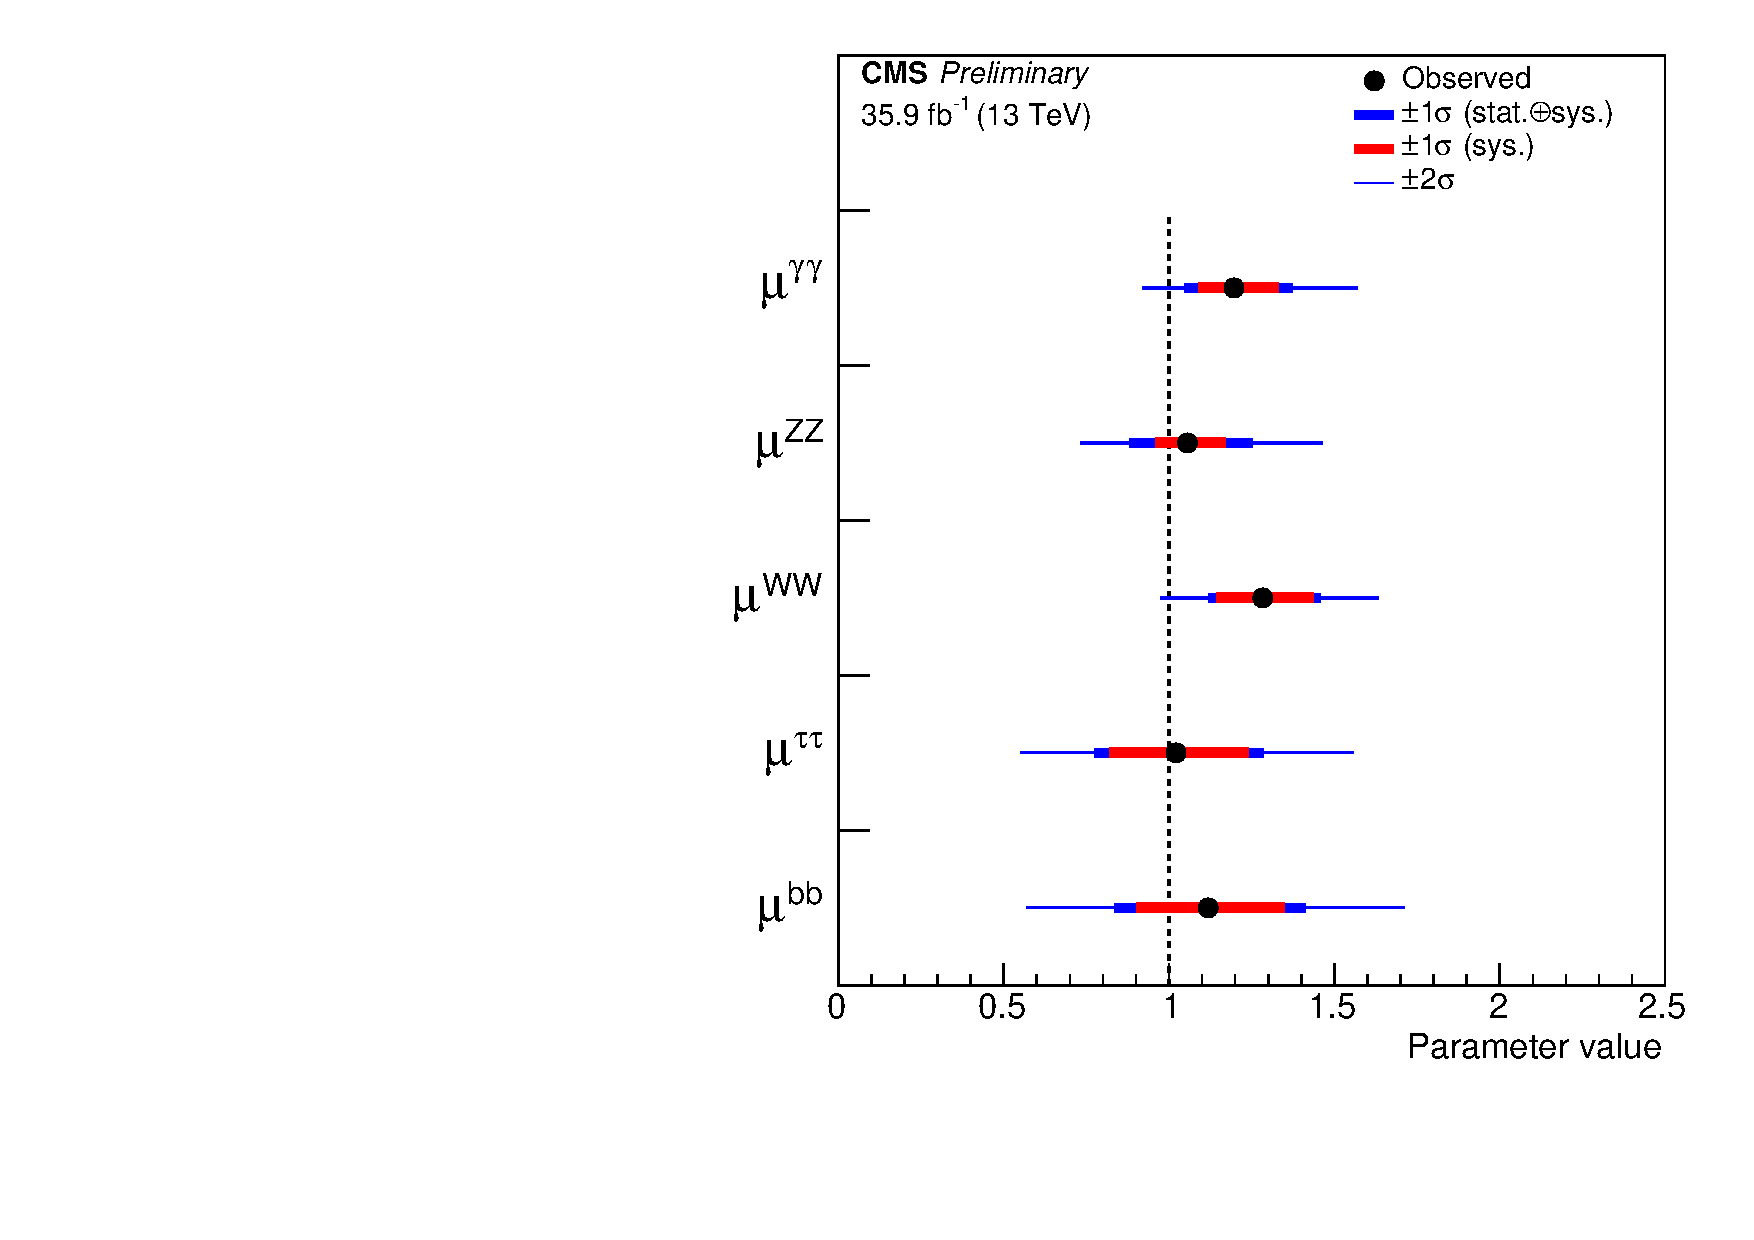
\includegraphics[width=0.54\textwidth]{Images/MuF}
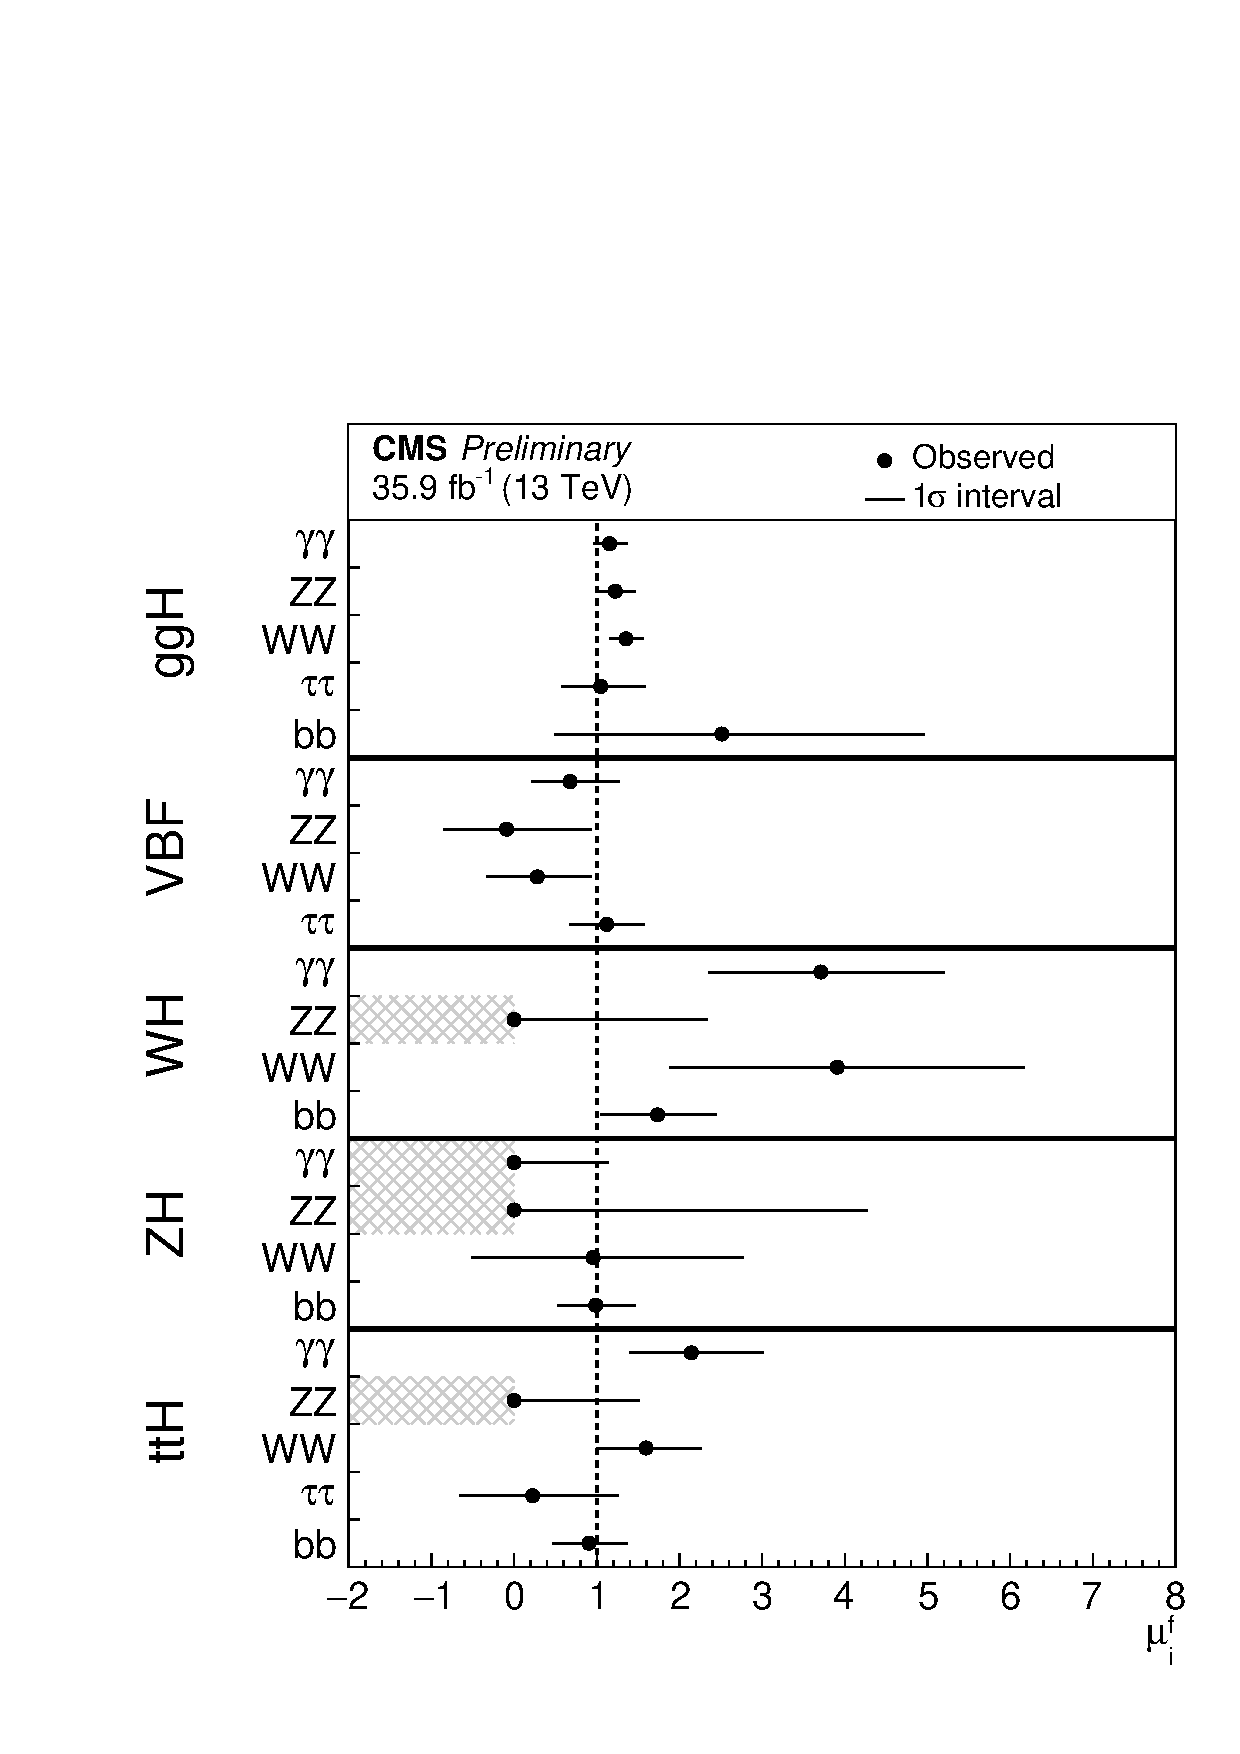
\includegraphics[width=0.45\textwidth]{Images/MuIeMuF}
\caption{Summary plot of the fit to the per-production mode (left) and per-decay mode (right) signal strength modifiers $\mu_i$. The thick and thin horizontal bars indicate the $\pm$1$\sigma$ and $\pm$2$\sigma$ uncertainties, respectively. Also shown are the $\pm$1$\sigma$ systematic components of the uncertainties. The last point in the per-production mode summary plot is taken from a separate fit and indicates the result of the combined overall signal strength $\mu$. On the bottom, summary plot of the fit to the production-decay signal strength products $\mu^f_i = \mu_i \times \mu^f$. The points indicate the best-fit values while the horizontal bars indicate the 1$\sigma$ CL intervals. The hatched areas indicate signal strengths which are restricted to positive values due to low background contamination.}
\label{SignalStrength}
\end{figure}
\subsubsection{Higgs coupling constant}
In order to test and parametrise for deviations in the couplings of the Higgs boson to other particles, a set of coupling modifiers, $\vec{\kappa}$, is introduced. For a given production process or decay mode j, a coupling modifier $\kappa_j$ is introduced:
\[
\kappa^2_j = \sigma_j/\sigma^{SM}_j,\ or\ \kappa^2_j = \Gamma^j/\Gamma_{SM}^j
\]
Under the assumption that there are no new particles contributing to the ggH production or $H\to \gamma\gamma$ decay loops, these processes can be expressed in terms of the coupling modifiers to the others SM particles. In this model six free coupling parameters are introduced: $\kappa_Z$, $\kappa_W$, $\kappa_t$, $\kappa_b$, $\kappa_\tau$, $\kappa_\mu$ and it is assumed that there is no BSM contribution to the total Higgs boson width. In the SM, all $\kappa^2_j$ values are positive and equal to unity: the results of the fits with this parametrisation are given in \figurename~\ref{Hkappa}.
\begin{figure}[htbp]
\centering
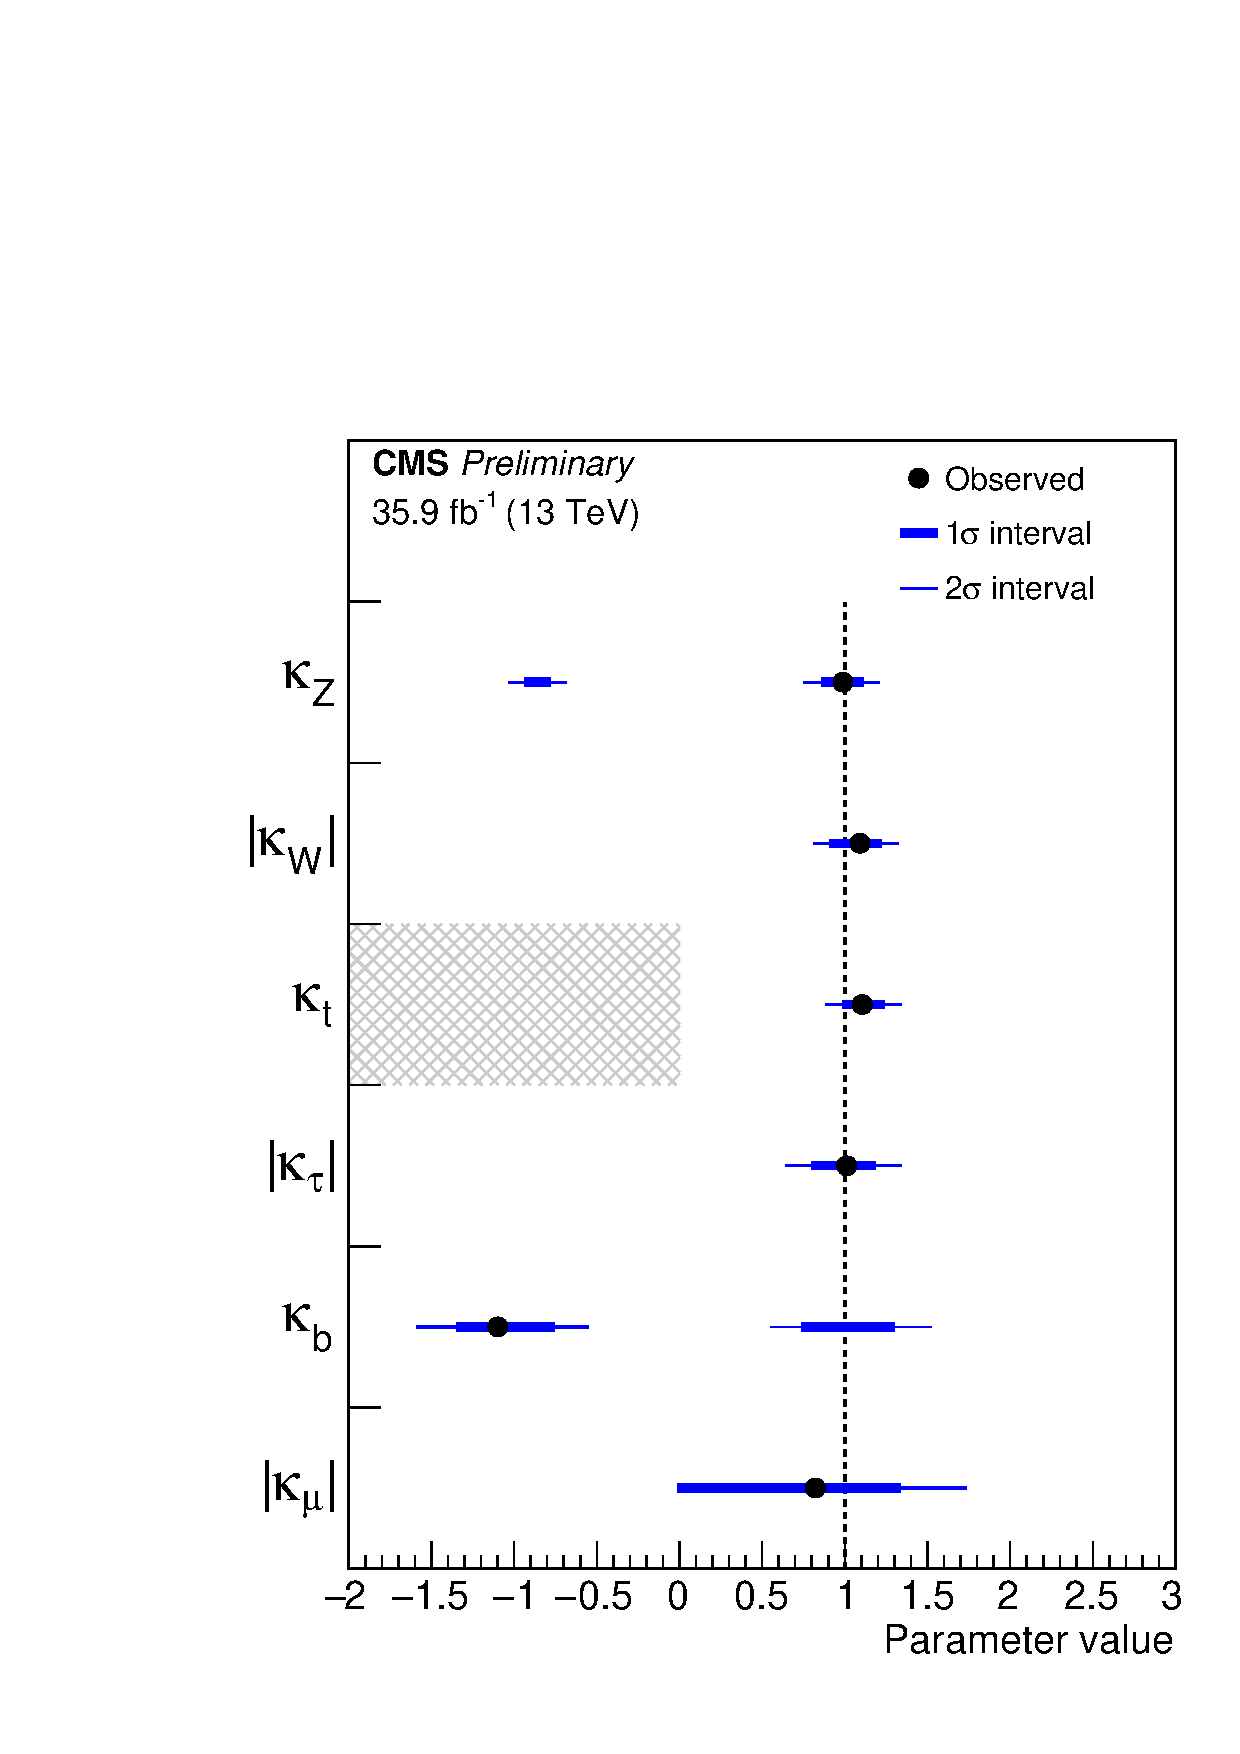
\includegraphics[width=0.45\textwidth]{Images/Hkappa}
\caption{Summary of the $\kappa$-framework model with $BR_{BSM} $= 0. The points indicate the best-fit values while the thick and thin horizontal bars show the 1$\sigma$ and 2$\sigma$ CL intervals, respectively. In this model, the ggH and H$\to\gamma\gamma$ loops are resolved in terms of the remaining coupling modifiers. For this model, both positive and negative values of $\kappa_Z$ and $\kappa_b$ are considered while $\kappa_W$ is assumed to be positive \cite{LatestHiggsCMS}.}
\label{Hkappa}
\end{figure}
An other way to fit the possible deviation to the SM in the Higgs coupling, is to parametrise $\kappa$ in term of other two parameters, M and $\epsilon$ \cite{Hcoupling1, Hcoupling2}. In this model one can relate the coupling modifiers to M and $\epsilon$ as $\kappa_F = \nu\ m_f^\epsilon / M^{1+\epsilon}$ for fermion of mass $m_f$ and $\kappa_V = \nu\ m_V^{2\epsilon} / M^{1+2\epsilon}$ for vector boson of mass $m_V$. In absence of BSM contribution, in the SM, $\kappa_i$ = 1 and considering $\nu$ = 246.22 GeV, (M, $\epsilon$) = ($\nu$, 0). In \figurename~\ref{Mespilon} are reported the 1$\sigma$ and 2$\sigma$ CL regions in the (M, $\epsilon$) fit. In order to show both the Yukawa and vector boson couplings in the same plot, a reduced vector boson coupling, $\sqrt{\kappa_V}\cdot m_V/\nu$, is shown.
\begin{figure}[htbp]
\centering
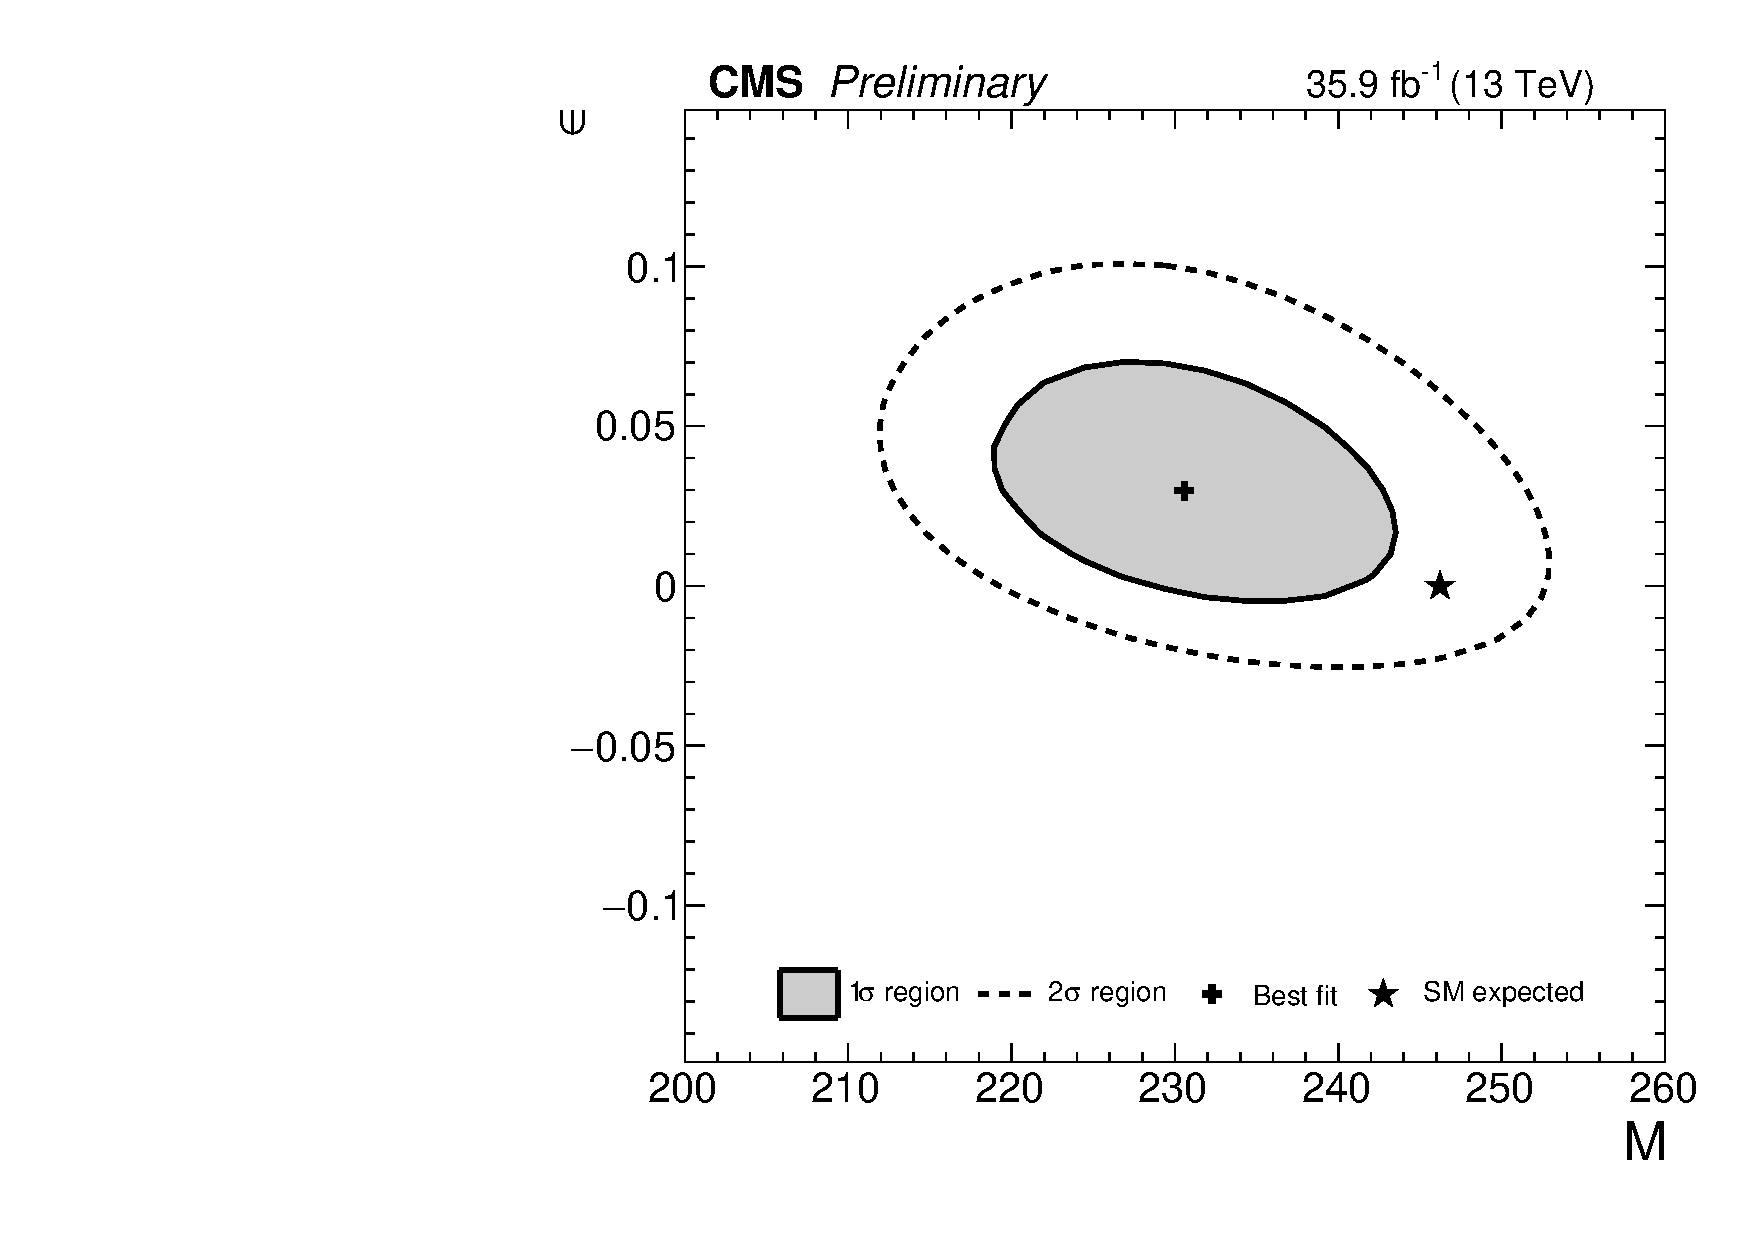
\includegraphics[width=0.45\textwidth]{Images/M_vs_epsilon}
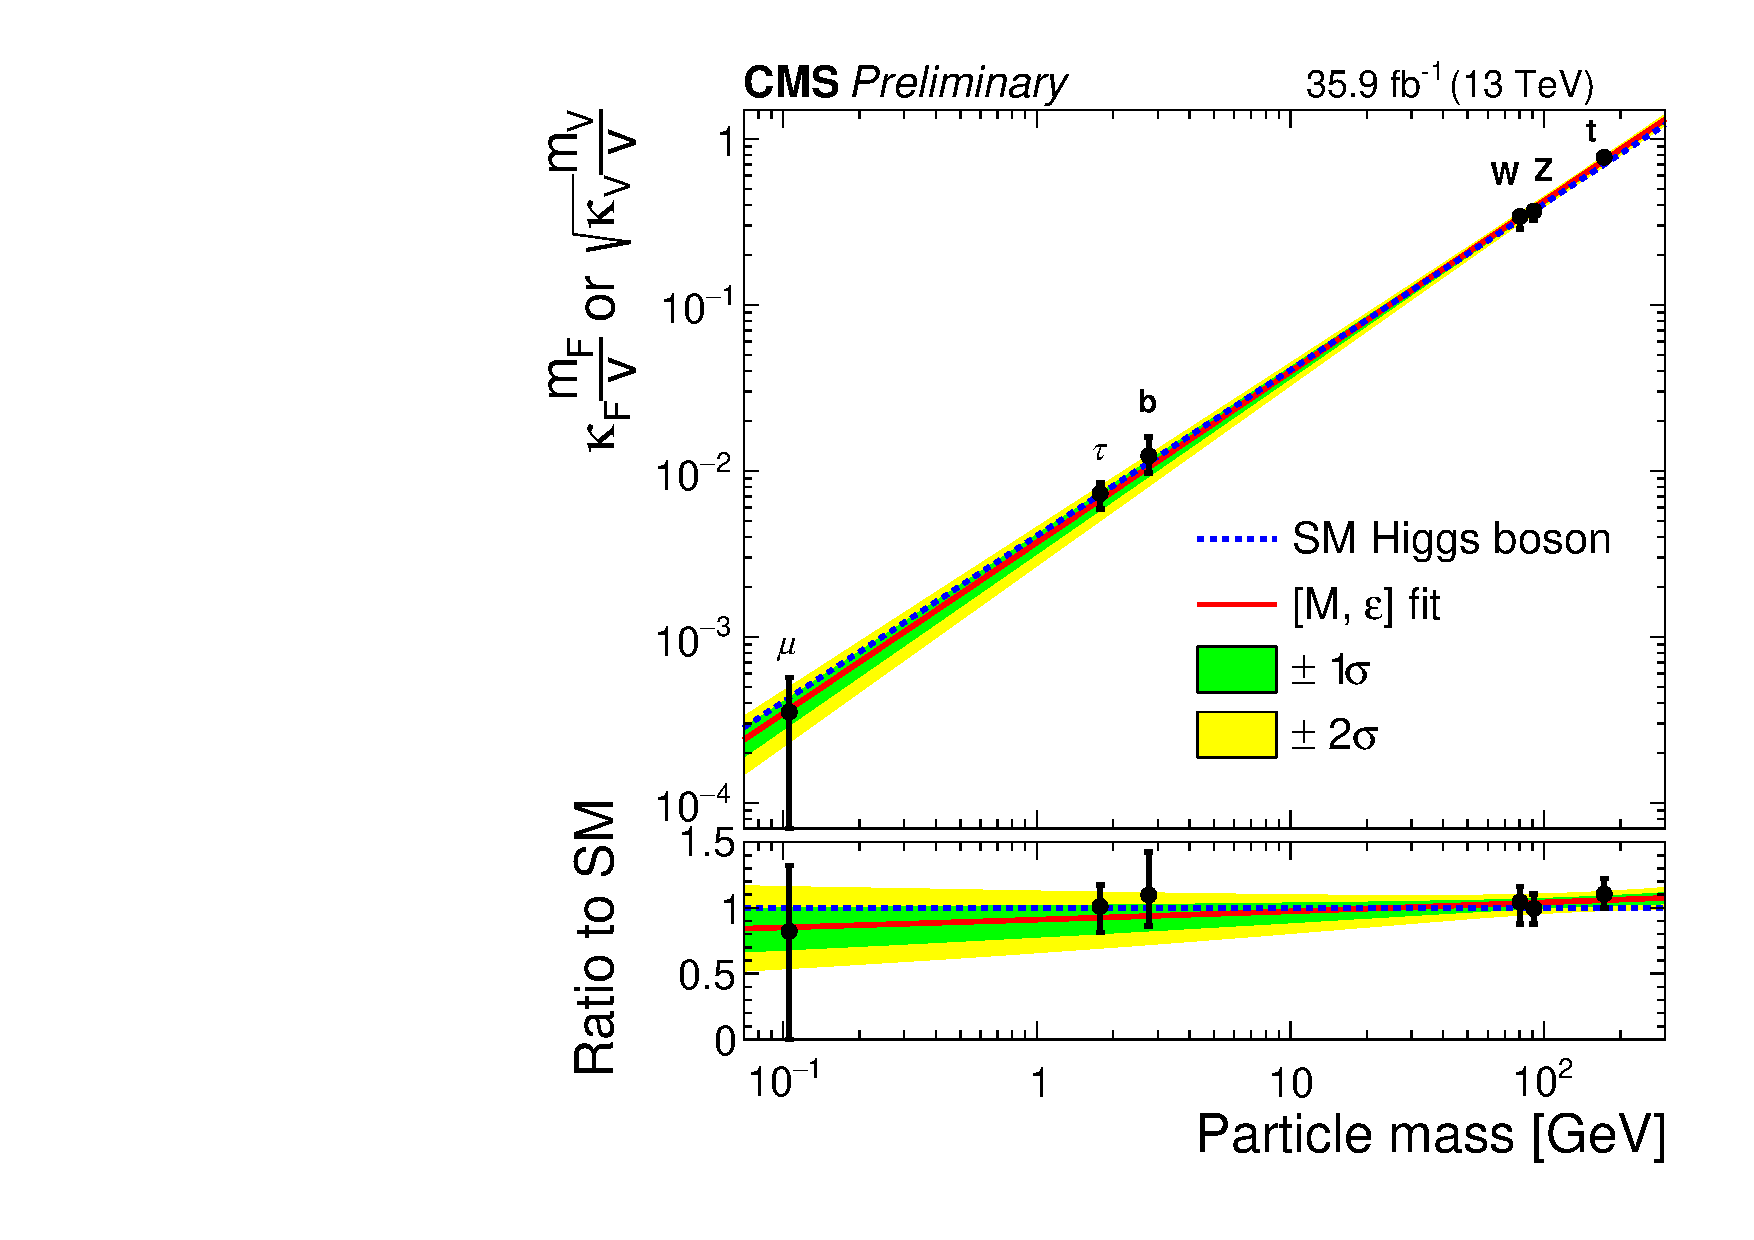
\includegraphics[width=0.45\textwidth]{Images/Hcoupling}
\caption{Left: Likelihood scan in the M-$\epsilon$ plane. The best-fit point and 1$\sigma$, 2$\sigma$ CL regions are shown, along with the SM prediction. Right: Result of the phenomenological M, $\epsilon$ fit overlayed with the resolved $\kappa$-framework model \cite{LatestHiggsCMS}.}
\label{Mespilon}
\end{figure}

\section{Beyond Standard Model (BSM)}
The SM aims to describe all fundamental interaction in a common way but at the same time, considering the gauge group symmetry \ref{gaugeMS}, it introduces three running coupling constants, whose value depends on the energy. In this view, it is expected to reach an energy value at which these three coupling constants converge but it can been demonstrated that, within the SM, this does not happen: \figurename~\ref{rccMS} shows coupling constants behaviour as a function of energy. 
\begin{figure}[htbp]
\centering
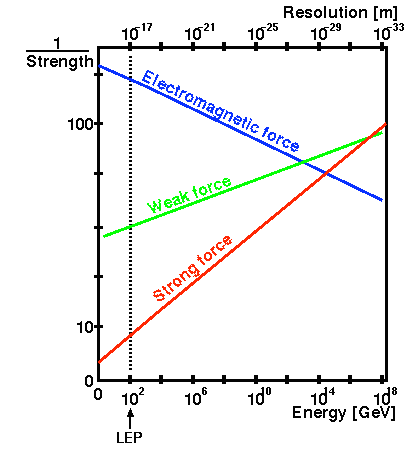
\includegraphics[width=0.45\textwidth]{Images/rccMS}
\caption{Evolution of the inverse of the three running coupling constants of the SM.}
\label{rccMS}
\end{figure}
This issue is only one of the open questions SM is not equipped to address: \eg it does not have a quantum description of the Gravity, treated currently only classically; it has no candidate for Dark Matter and no explanation for Dark energy (constitute around 96\% of the Universe). An other problem, linked with the Higgs boson mass within the SM, is the so called "hierarchy problem": in the theory, the Higgs boson receives quantum corrections from heavy particles. While the Higgs boson has a mass $m_H\approx$125 GeV, the corrections are of the order of the Planck mass, $M_P = \sqrt{\hbar c /G} \approx10^{19}$GeV, and not, as one might expect, of the same order of $m_H$. \\
With the aim to try to solve these issues, many models beyond SM (BSM) have been developed, introducing new particles/interactions and more symmetries. The easiest way to do this, is to consider a larger unification groups. \\

\subsection{Sequential Standard Model}
The Sequential Standard Model (SSM) predicts the existence of a new boson, Z$'_{SSM}$, with the same features of the SM Z boson \cite{Z_SSM}. In this model, the decay width of the boson into a pair of fermions is given by:
\[
\Gamma(Z'_{SSM}\to f\bar{f}) = \frac{\alpha}{48}N_C\frac{M_{Z'_{SSM}}}{\sin^2\theta_W\ \cos^2\theta_W}[1+(1-4|Q_f|cos^2\theta_W)^2]
\]
where, $\alpha$ is the fine-structure constant, $N_C$ is the number of colors applicable for that fermion, $\theta_W$ is the Weinberg angle and $Q_f$ is the electric charge of the fermion.
This is often used as a benchmark model for experimental Z$'$ searches.

\subsection{Grand Unified Theories}
Grand Unified Theories, GUT's \cite{GUT}, try to describe all fundamental interaction by one simple gauge group G at very high energies $E> E_{GUT}$. For energy $E\ll E_{GUT}$ the gauge group must be broken and obtain the SM gauge symmetry group \ref{gaugeMS}, similar to the breaking of the $SU(2)_L\times U(1)_Y$ symmetry to $U(1)_{em}$ in the SM which occurs at $E_{weak} $= O(100GeV). The smallest simple gauge group G which can contain the SM is G = SU(5) with 4 neutral gauge bosons.  \\
GUT can be tested measuring proton decay: to be consistent with present experiments on proton decay,  $E_{GUT}>10^{15}$ GeV, much larger than $E_{weak}$ and smaller than the Planck mass, $M_P$. At energies above the Planck mass, Gravity is expected to become as strong as the other interactions. At energies well below $M_P$, as it happens in GUT, the effects of Gravity can be neglected. $E_{GUT}$ is also predicted as the energy where the three running gauge coupling constants of the SM gauge group become equal.
All GUT's with gauge groups larger than SU(5) predict at least one extra neutral gauge boson (Z$'$). \\
The next interesting gauge group larger then SU(5) is SO(10). The SO(10) theory predicts one extra neutral gauge boson because rank[SO(10)] = 5. \\
More interesting is the case of $E_6$: when it is broken, to the effective strong-electroweak group at low energy, different models are possible. The gauge group $E_6$ is broken at the GUT scale to SO(10) and a $U(1)_\psi$ gauge group
\[
E_6 \to SO(10) \times U(1)_\psi
\]
The SO(10) is further broken at the GUT scale to SU(5) and a $U(1)_\chi$ gauge group,
\[
SO(10) \to  SU(5) \times U(1)_\chi
\]
Finally the SU(5) is broken at the GUT scale to the Standard Model (SM) gauge group, \ref{gaugeMS}. \\
For the linear combination 
\[
U(1)' = U(1)_\chi \cos\theta  + U(1)_\psi \sin\theta 
\]
is possible for the two generators, $T_\psi$ and $T_\chi$ to survive down to the TeV scale. \\
At different value of the mixing angle $\theta$, free parameter of the theory, corresponds different Z$'$ phenomenology. The most widely used models, with their corresponding mixing angle, are: $Z'_\psi$ ($\theta$=0),  $Z'_\chi$ (-$\pi$/2), $Z'_\eta$ ($\arccos(5/8)$) and  $Z'_I$ ($\arccos(5/8)-\pi/2$). \\
These theories unify the three gauge interactions of the Standard Model but at the same time they leave unanswered most of the open questions above, except for the fact that reduce the number of independent parameters due to the fact that there is only one gauge coupling at large energies. 

\subsection{Extra dimensions model}
%One way to solve the hierarchy problem, is to suppose that there are n extra compact spatial dimensions of radius $\sim$ R \cite{ExtraDimentions}. \\
While electroweak interactions have been probed at distances $\sim m^{-1}_{EW}$, gravitational forces have not remotely been probed at distances  $\sim m^{-1}_{Pl}$
and Gravity has only been accurately measured in the $\sim$ 1cm range. The interpretation of $M_{P}$ as a fundamental energy scale (where gravitational interactions become strong) is then based on the assumption that Gravity is unmodified over the 33 orders of magnitude between where it is measured at $\sim$1 cm down to the Planck length $\sim10^{-33}$ cm. This reasoning leads to the idea of abandoning the interpretation of $M_{P}$ as a fundamental energy scale, and leaving only $m_{EW}$ as fundamental scale. To account for the observed weakness of Gravity compared to electroweak interactions, new n extra compact spatial dimensions of radius $\sim$ R are introduced, with Gravity being the only fundamental interaction that sees them \cite{ExtraDimentions}. 
%The SM fields are trapped on a 4-dimansional wall, often called a brane in the extra dimensions, and gravitons are the only particles freely propagating in the whole space (the bulk). \\
Two test masses of mass $m_1$, $m_2$ placed within a distance r$\ll$ R will feel a gravitational potential dictated by Gauss's law in (4 + n) dimensions:
\[
V(r) \sim \frac{m_1m_2}{M^{n+2}_{P(n+4)}} \frac{1}{r^{n+1}}
\]
If now, the masses are placed at distances r $\gg$ R, their gravitational flux lines can not continue to penetrate in the extra dimensions, and the usual 1/r potential is obtained:
\[
V(r) \sim \frac{m_1m_2}{M^{n+2}_{P(n+4)}R^n} \frac{1}{r}
\]
so our effective 4 dimensional $M_{P}$ is
\[
M^2_{P} \sim M^{n+2}_{P(n+4)}R^n
\]
The fundamental Planck mass can, thus, be in the TeV range, which would solve the hierarchy problem. The observed strength of Gravity can be reproduced with a suitable choice of R and n. If one assumes the mass scale at 1 TeV, a condition for the size of the extra dimension arises
\[
R \sim 10^{\frac{30}{n}-17}\ cm \times \frac{1\ TeV}{m_{EW}}^{1+\frac{n}{2}}
\]
%The case n =1 (R $\sim 10^{13}$ cms) and n = 2 (R $\sim$ 1mm) are empirically excluded. 
While the SM gauge forces have been accurately measured at weak scale distances, Gravity has not been probed at distances smaller than a millimeter: this means the SM particles cannot freely propagate in the extra n dimension, but must be localized to a 4 dimensional world having a thickness $\sim m_{EW}^{-1}$ in the extra n dimensions. The only fields propagating in the (4 + n) dimensional bulk is the (4 + n) dimensional graviton, with couplings suppressed by the (4 + n) dimensional Planck mass $\sim m_{EW}$.

\subsubsection{Randall-Sundrum model and Kaluza-Klein tower}
Let's consider, in the case n = 1, a massless (4+1)D scalar field $\phi^{M}$ with M= {0,1, ..., 4} with action
\begin{equation}
S_{5D} = \int d^5x\ \partial^M\phi \partial_M\phi
\label{5D_action}
\end{equation}
Set the extra dimension $x^4$ = y defining a circle of radius r with y $\equiv$ y + 2$\pi$r. The periodicity in y direction implies discrete Fourier expansion
\begin{equation}
\phi(x^{\mu}, y) = \sum_{n=-\infty}^\infty \phi_n(x^\mu)\ e^{iny/r}
\label{5D_Fourier}
\end{equation}
Notice that the Fourier coefficients are functions of the standard 4D coordinates and therefore are (an infinite number of) 4D scalar fields. The equations of motion for the Fourier modes are (in general massive) wave equations
\[
\partial^\mu\partial_\mu\phi_n(x^\mu)-\frac{n^2}{r^2}\phi_n(x^\mu) = 0
\]
These are then an infinite number of Klein Gordon equations for massive 4D fields. This means that each Fourier mode $\phi_n$ is a 4D particle with mass $m^2_n = \frac{n^2}{r^2}$. Only the zero mode (n = 0) is massless. One can visualise the states as an infinite tower of massive states (with increasing mass proportional to n). This is called Kaluza Klein (KK) tower and the massive states (n $\ne$ 0) are called Kaluza Klein or momentum states, since they come from the momentum in the extra dimension.
Substituting \ref{5D_Fourier} in \ref{5D_action}, can be demonstrated that the 5D action reduces to one 4D action for a massless scalar field plus an infinite sum of massive scalar actions in 4D. \\
In the Randall-Sundrum model \cite{RandallSundrum}, the fifth dimension y is confined in $0 < y <2\pi$ with the additional condition ($x^\mu$, y) $\equiv$ ($x^\mu$, -y). The solution to Einstein's equations in such 5-dimensional space is an anti-de Sitter (AdS5) space with non-factorizable geometry, given by the metric 
\[
ds^2 = e^{-2kr_c|y|}\eta_{\mu\nu}dx^\mu dx^\nu+r_c^2dy^2
\]
where k $\sim M_P$ is the AdS5 curvature parameter, $r_c$ is the compactification radius and $\eta_\mu\nu$ is the 4-dimensional metric tensor. Assuming that the SM fields are confined to the brane located at y = $\pi$, any fundamental 5-dimensional mass parameter $m_0$, has an effective 4-dimensional value of
\[
m = e^{-kr_c\pi}m_0
\]
This gives rise to massive leptonically decaying KK gravitons in the 4- dimensional world, with masses at the TeV scale, easily generated from parameters of order of the Planck scale. The compactification scale 1/$r_c$ is of the order of $M_P$, so no additional hierarchy is introduced and the masses of KK excitations modes are
\[
m_n = kx_ne^{-kr_c\pi}
\]
where $x_n$ is the n-th root of the $J_1$ Bessel function. The Randall-Sundrum model phenomenology is governed by two free parameters, with the mass of the first graviton excitation $m_1$ ($M_{G_{KK}}$ in the future) and the coupling parameter of the graviton to the SM, c = k/$\bar{M}_P$\footnote{$\bar{M}_P$ is the reduce Planck mass defined as $M_P/\sqrt{8\pi}$}
as being the usual choice . 
% it does not have a satisfactory mechanism for generating neutrino masses and does not explain or stabilise the hierarchy of mass scales in physics. In order to try to solve these issues many models have been developed beyond standard model.\\
%The easiest way to extend the SM it with and additional U(1)' group with the associated Z' gauge boson.

\subsection{Dark Matter Model}
Many models have been developed to describe how Dark Matter (DM) can be produced: these models involve TeV-scale mediating particles that couple to quarks and a Dirac fermion DM candidate. \\DM does not interact with ordinary matter and this means that it does not leave any tracks in the detector: it looks like a neutrino. This leads to search for a large missing transverse energy as possible signal signature. An other possibility to detach DM is to look at the decay product of the mediator particle DM-SM: in a simplified model, this mediator is a  vector or an axial-vector spin-1 high-mass boson \cite{DarkMatter}, exchanged via $s$ channel. This model has four free parameters: the DM mass $m_{DM}$, the mediator mass $M_{med}$, the coupling $g_{DM}$ of a mediator-DM-DM vertex, and the coupling $g_q$ universal to all mediator-quark-quark vertices; a fifth free parameter, the lepton coupling $g_l$ can be introduced. These five parameters define the production rate of the mediator, its DM and leptonic/hadronic decay rates, and the kinematics of the signal event.  \\







\begin{comment}
Consider a simple case of a Lagrangian describing a scalar particle:
\begin{equation}
\mathcal{L} \equiv T - V = \frac{1}{2}(\partial \phi)^{2}-(\frac{1}{2}\mu^{2}\phi^{2} + \frac{1}{4}\lambda\phi^{4})
\label{L0}
\end{equation}
with $\lambda > 0$; keeping the first two allowed terms in the general expansion of V in power of $\phi$ guarantee \ref{L0} to be invariant under the symmetry operation $\phi \to -\phi$. 
The two possible form of the potential are shown in \figurename~\ref{V_phi_potential}
\begin{figure}[htbp]
\centering
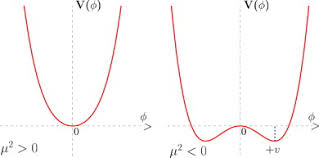
\includegraphics[width=0.45\textwidth]{Images/V_phi_potential}
\caption{The potential $V(\phi) = \frac{1}{2}\mu^{2}\phi^{2} + \frac{1}{4}\lambda\phi^{4}$ for (a) $\mu^{2} > 0$ and (b) $\mu^{2} < 0$.  \textbf{CAMBIA IMMAGINE: FA SCHIFO}}
\label{V_phi_potential}
\end{figure}
In the case $\mu^{2}$ is positive, the ground state (the vacuum) correspond to $\phi = 0$ and obeys the reflection symmetry of the Lagrangian. More interesting is the case in which $\mu^{2}$ is negative and the potential has two minima:
\begin{equation}
\phi = \pm\nu \quad\ with\ \nu = \sqrt{-\mu^{2}/\lambda}
\end{equation}
Perturbative calculations should involve expansions around the classical minimum\footnote{choosing $\phi = \nu$ does not imply any loss of generality since $\phi = -\nu$ can always be reached by reflection symmetry.}:
\begin{equation}
\phi(x) = \nu + \eta(x)
\label{phi_perturbative}
\end{equation}

\end{comment}


\selectlanguage{english}
\chapter{The CMS detector at LHC}
\label{Chapter2}
%SourceDoc tesi.tex

\section{The Large Hadron Collider}
Approved in the early '90s and started up in the 2008, the \textit{Large Hadron Collider} (LHC)  is currently the world's largest and most powerful particle accelerator. \\
Its main purpose is to help in testing the predictions of different theories of particle physics. \\
%, including the search of the Higgs boson and the dark matter. \\
LHC \cite{LHC},  situated at the CERN laboratories of Geneva, is a proton-proton (pp) collider built to work at the design center of mass energy of $\sqrt{s} = 14$ TeV, with a bunch crossing every 25 ns and a design luminosity of $10^{34}$ cm$^{-2}$ s$^{-1}$. It is  installed in the same circular underground tunnel occupied until the year 2000 by the Large Electron Positron
collider (LEP). The $pp$ collision are used, instead of the $e^+e^-$ one of LEP, to reduce the synchrotron radiation, in order to accelerate the particles up to a very large energy. It was preferred to a $p\bar{p}$ collider because it allows to reach higher rate of events. In fact the low anti-proton production efficiency ($10^5$ protons are needed to create an anti-proton) and larger time needed to accumulate them, would make almost impossible to reach the high design luminosity of the LHC. The luminosity $L$ is the parameter to quantify the performances of a collider, because the event rate $R_i$ of a given process $i$, defined as the number of events occurring per unit of time, can be written as:
\begin{equation}
R_i = \frac{dN_i}{dt}=L\cdot \sigma_i
\end{equation}
where $\sigma_i$ is the cross section of the process $i$. The luminosity depends only on the machine parameters. Assuming a small crossing angle between the
beams and Gaussian-shaped beam bunches, the luminosity $L$ can be written as:
\begin{equation}
L=\frac{fn_bN^2}{4\pi\sigma^2}
\end{equation}
where $f$ is the revolution frequency of particle bunches, $n_b$ is the number of bunches rotating in the accelerator, $N$ is the number of protons in the two colliding bunches and $\sigma$ is the RMS of beam profile distributions in the plane orthogonal to the beam direction. \\
%LHC is a 26.7 km ring of superconducting magnets with a number of accelerating structures to boost the energy of the particles along the way. It is not a perfect circle: it is made of eight arcs and eight insertions. The arcs are long 106.9m with a curvature of 2.84km containing 1232 superconductive dipoles. The LHC dipoles use Niobium-Titanium (NbTi) cables at a temperature of 1.9K, pumping superfluid helium into the magnet system, where they become superconducting; a current of 11850A flows in the dipoles to create the high magnetic field of 8.33 T required to bend the beams around the ring. The insertions instead consist of a long straight section of 528m plus two (one at each end) transition regions. They contains the radiofrequency cavities to increase beam energy (0.5 MeV per period): there are eight cavities per beam, each delivering 2MV (an accelerating field of 5MV/m) at 400MHz operating at 4.5K. Particular kind of insertion are quadrupoles, special magnets used to focus the beam down to the smallest possible size at the collision points: there 392 quadrupoles in LHC. The two beams will run in two contiguous pipes with vacuum inside, separated by 19.4 cm, that will be unified in proximity of the interactions points, where the experiments will be placed. Because of the high luminosity of the LHC, large thermal power will be generated near the pipes due to the synchrotron radiation, making necessary the presence of a suitable cooling system. For this reason also the pipes will be in contact with superfluid Helium at 1.9 K. \\
In the LHC design, 1232 main dipole magnets (made of niobium-titanium super-conductor chilled with superfluid Helium at 1.9 K) generating a magnetic field up to 8.3 T, will be used to steer the particles into curvilinear trajectories. The two beams will run in two contiguous pipes with vacuum inside, separated by 19.4 cm, that will be unified in proximity of the interactions points, where the experiments will be placed. Because of the high luminosity of the LHC, large thermal power will be generated near the pipes due to the synchrotron radiation, making necessary the presence of a suitable cooling system. For this reason also the pipes will be in contact with superfluid Helium at 1.9 K. \\
In \figurename~\ref{Cern-Accelerator-Complex}  is shown the complete scheme of the accelerator chain of the LHC: the proton beam is created by using an electric field to pull the electrons from hydrogen atoms and start the acceleration. Protons are injected into the PS Booster (PSB) at an  energy of 50 MeV from Linac2 (Linear Accelerator 2). The booster comprises four superposed rings: this is because at low energy intensity, the quality of the beams suffers from the repulsive forces between particles. By splitting up the injected beam this effect gets reduced. Once the beam reaches the energy of 1.4 GeV it is extracted and injected into Proton Synchrotron (PS). With a circumference of 628 m, the PS accelerates the beams up to 26 GeV when they are extracted and sent to the Super Proton Synchrotron (SPS). Built in the '70, the SPS has a length of 7 km. The beam is injected at 26 GeV, ramped up to 450 GeV and extracted to the LHC. \\%At the SPS, the boson W and Z were discovered and this led Rubbia and Simon van der Meer to win the Nobel prize. \\
\begin{figure}[htbp]
\centering
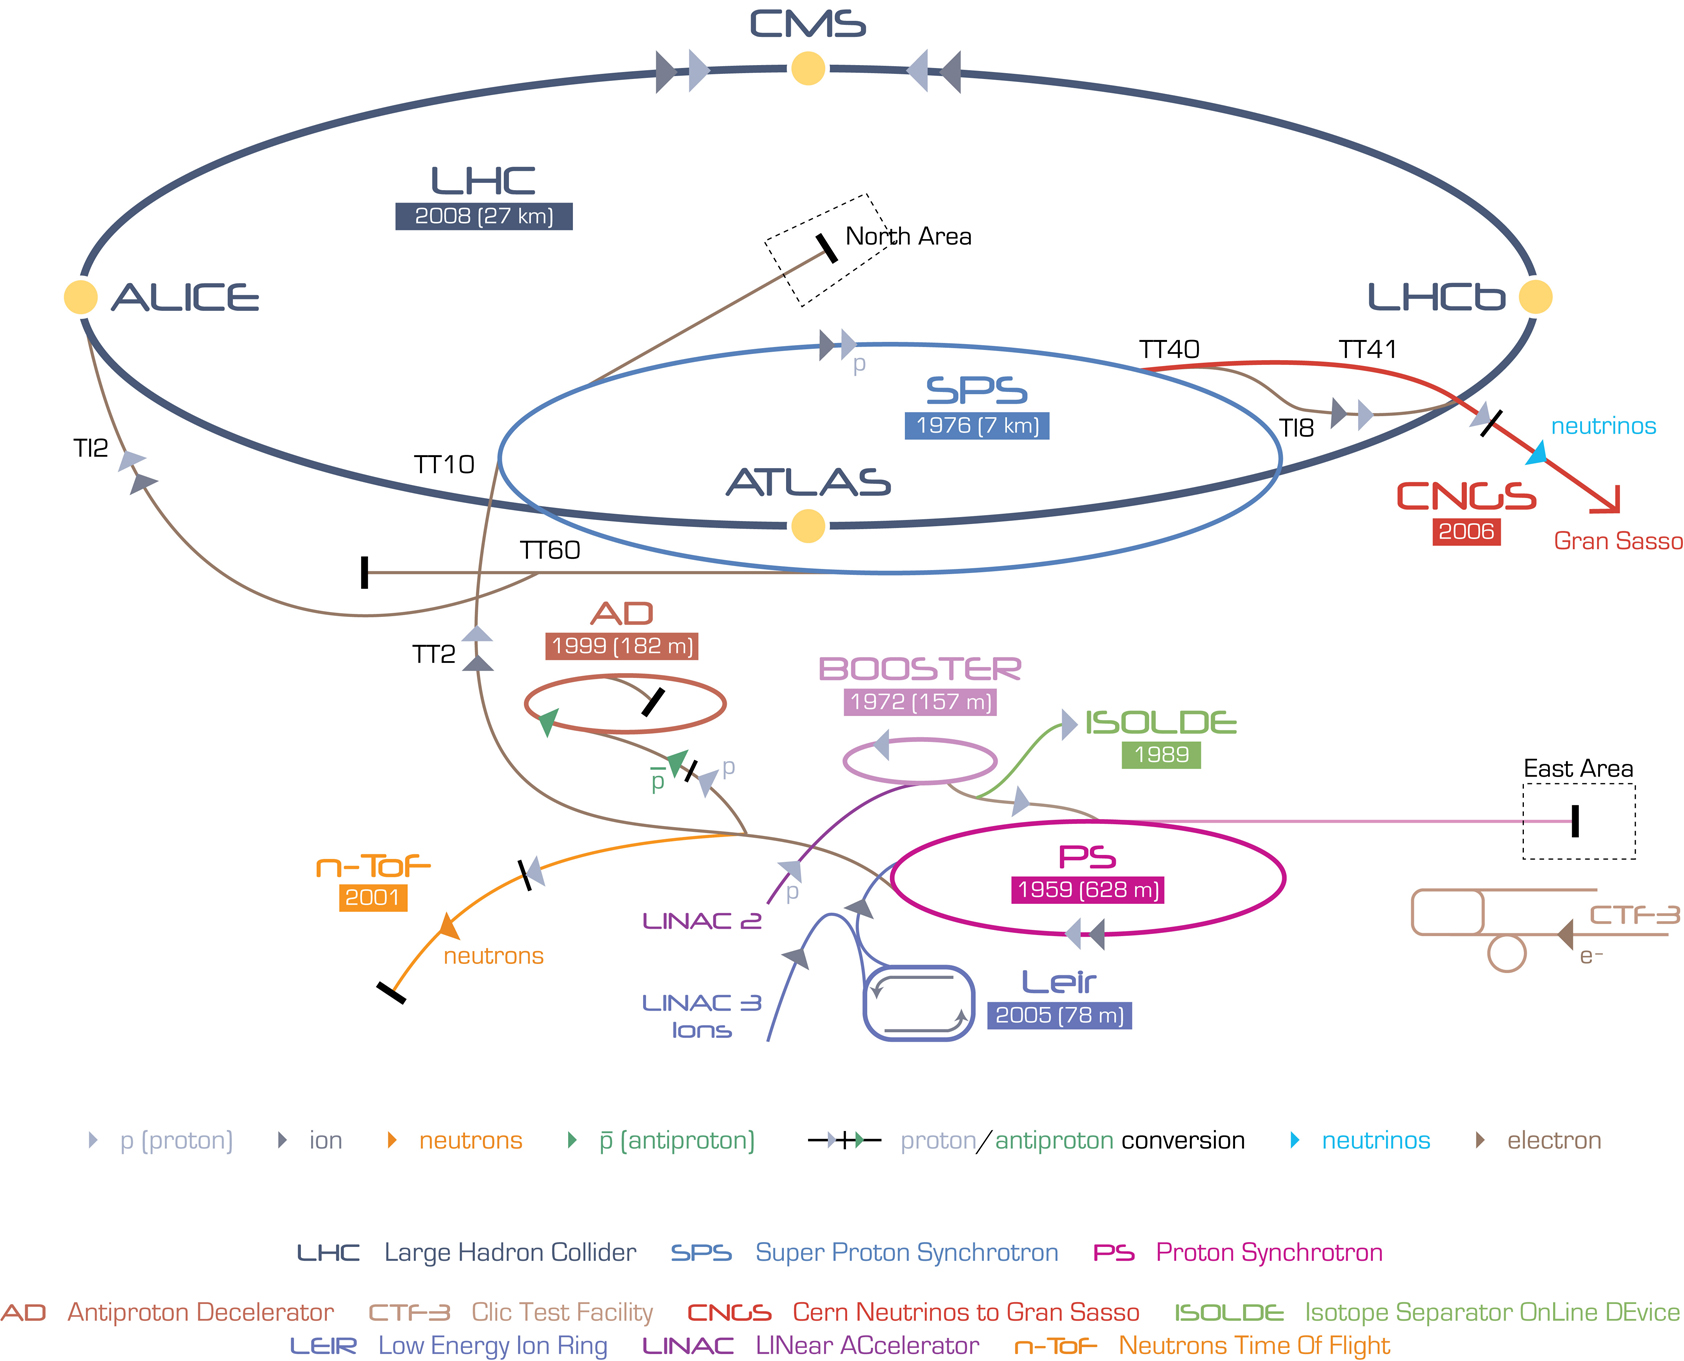
\includegraphics[width=0.65\textwidth]{Images/Cern-Accelerator-Complex}
\caption{Accelerator scheme at CERN.}
\label{Cern-Accelerator-Complex}
\end{figure}
Once the energy-working point is reached, the beams are made to collide at four locations around the LHC, corresponding to the position of four particles detectors: ALICE (\emph{A Large Ion Collider Experiment}), ATLAS (\emph{A Toroidal LHC ApparatuS}), CMS (\emph{Compact Muon Solenoid}) and LHCb (\emph{Large Hadron Collider beauty}). In addition to these, there are other three experiment installed at the LHC: TOTEM (\textit{TOTal Elastic and diffractive cross section Measurement}) installed close to CMS, MoEDAL (\textit{Monopole and Exotics Detector at the LHC}) close to LHCb and LHCf (\textit{Large Hadron Collider forward}) near ATLAS. \\
The beams at LHC have a bunch structure as a direct consequence of the radio frequency acceleration scheme. Protons can only be accelerated when the RF field has the correct orientation when particles pass through an accelerating cavity. Under nominal operating conditions, each proton beam has 2808 bunches, with each bunch containing about $10^{11}$ protons. The bunch size is not constant around the ring getting squeezed as much as possibile around the interaction points in order to increase the probability of collision. They measure a few centimetres long and a millimetre wide when they are far from a collision point; as the bunches approach  the collision points, they are squeezed to about $20\ \mu m$. LHC uses a bunch spacing of 25 ns (or 7.5 m) corresponding to a frequency of 40 MHz. \\
In \tablename~\ref{LHC_parameteres} are reported the designed LHC parameters and the ones reached at the end of RunII in 2018.
\begin{table}[htbp]	
	\begin{center}
		\begin{tabular}{p{6cm}*{3}{c}}
			\hline   &  & Design & 2018  \\
			\hline
			\hline
			\bfseries Centre of mass energy & \emph{E} & 14 TeV & 13 TeV \\
			\hline
			\bfseries Luminosity & \emph{L} & 10$^{34}$ cm$^{-2}$s$^{-1}$ & --- \\
			\hline
			\bfseries Time spacing &  & 25 ns & 25 ns\\
			\hline
			\bfseries Num. of bunches& \emph{k$_{B}$} & 2808 & ---\\
			\hline
			\bfseries Num. protons per bunch & \emph{N$_{p}$} & 1.15$\times$10$^{11}$ & ---\\
			\hline
			\hline
		\end{tabular}
	\end{center}
	\caption{LHC parameters}
	\label{LHC_parameteres}
\end{table}


\section{The Compact Muon Solenoid}\label{sec:cms}
The Compact Muon Solenoid (CMS) is one of the general purpose experiments which takes data at the LHC. Its physics goals range from the search for the Higgs boson to the searches for physics beyond the Standard Model, to the precision measurements of already known particles and phenomena \cite{CMS_Detector}. \\
The overall layout of CMS is shown in \figurename~\ref{CMS_Layout}. The inner tracker and the two calorimeters of CMS are located inside a $13\,$m-long, $5.9 \,$m inner diameter, $3.8\, $T superconducting solenoid. In order to achieve good momentum resolution within a compact spectrometer  without making stringent demands on muon-chamber resolution and alignment, a high magnetic field was chosen. The return field is large enough to saturate $1.5 \,$m of iron, allowing four muon stations to be integrated to ensure robustness and full geometric coverage. The central part of CMS is called \emph{barrel} while the two edges of the detector are denoted as \emph{endcaps}.
\begin{figure}[htbp]
\centering
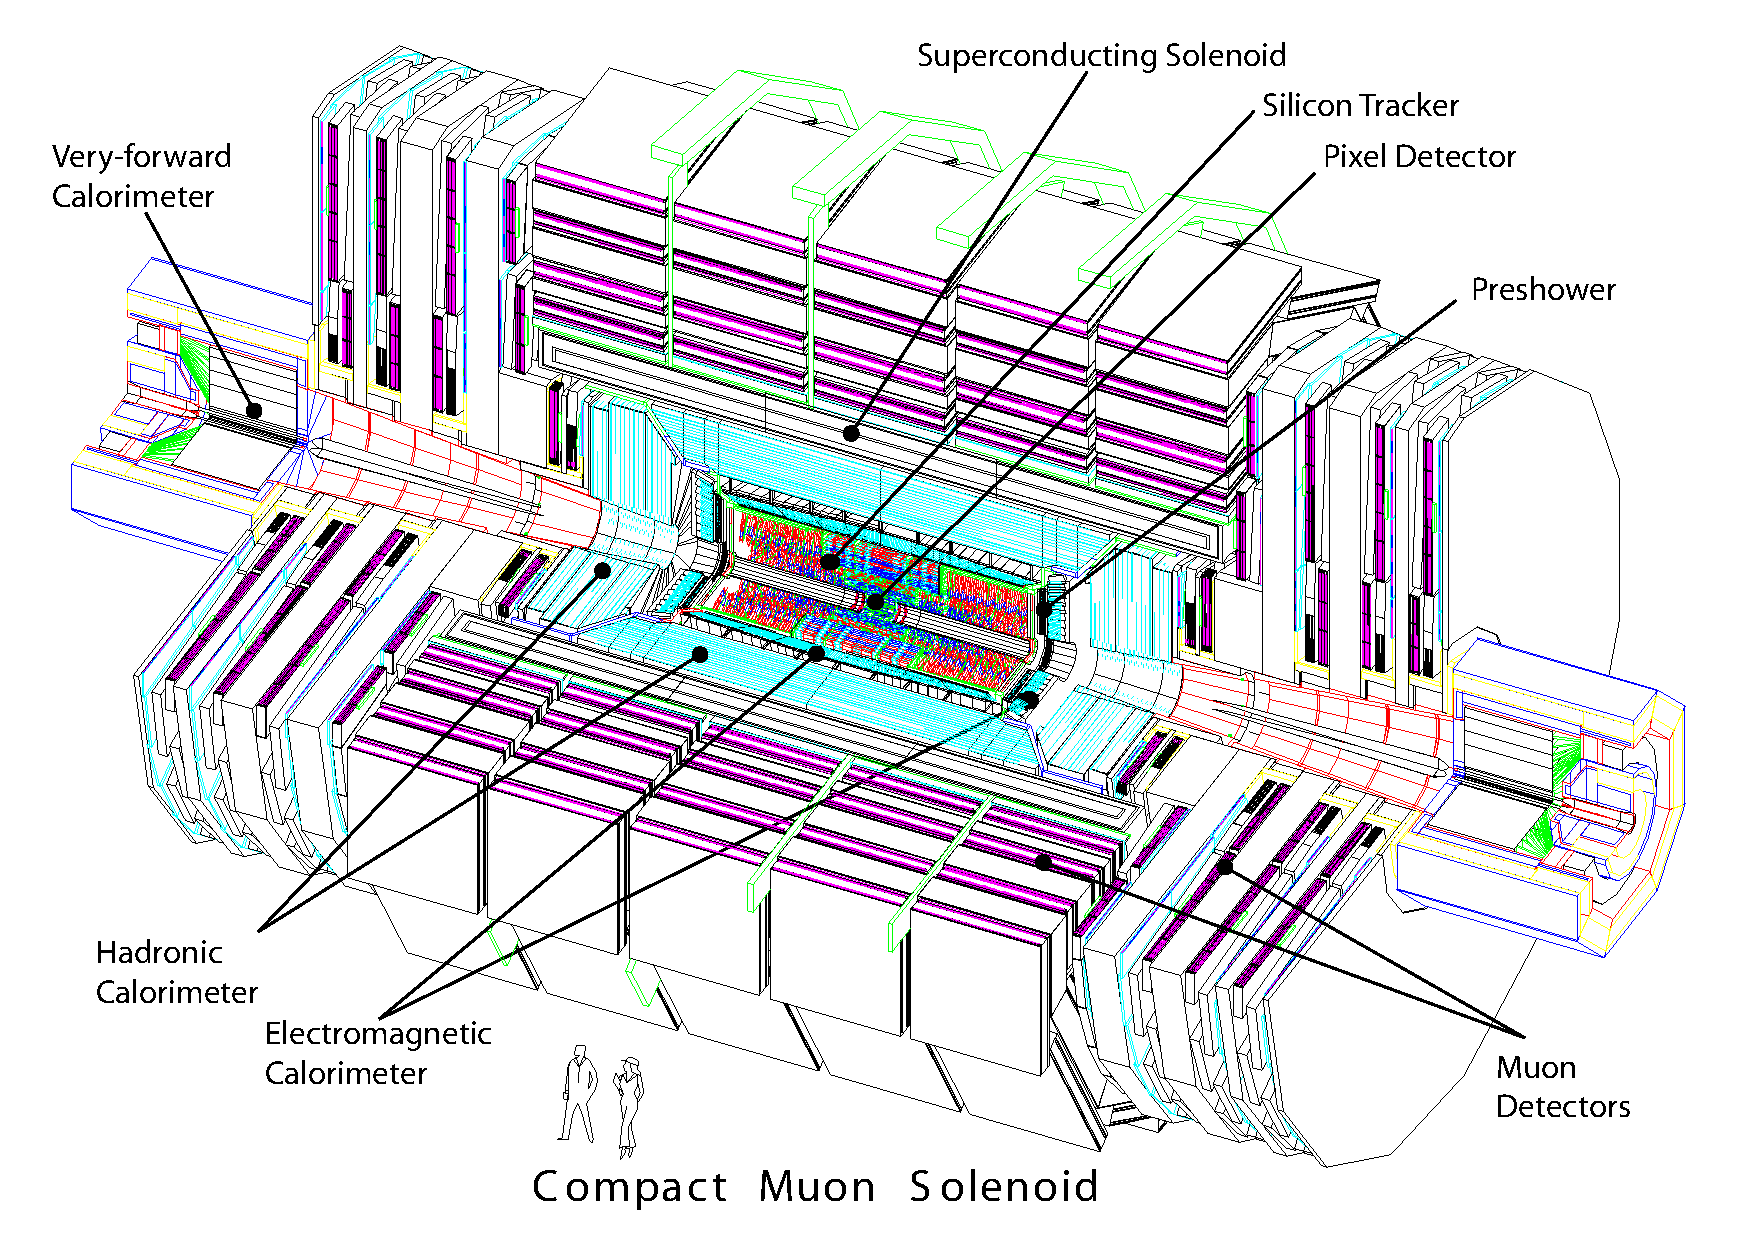
\includegraphics[width=0.7\textwidth]{Images/CMS_Layout.pdf}
\caption{CMS detector overview.}
\label{CMS_Layout}
\end{figure}
The tracking volume is given by a cylinder of length $5.8 \,$m and diameter $2.6 \,$m. In order to deal with high track multiplicities, CMS employs $10$ layers of silicon microstrip detectors, which provide the required granularity and precision. In addition, $3$ layers of silicon pixel detectors are placed close to the interaction region to improve the measurement of the impact parameter of charged-particle tracks, as well as the position of secondary vertexes. The electromagnetic calorimeter (ECAL) uses lead tungstate ($\mathrm{PbWO_4}$) crystals with coverage in pseudorapidity up to $|\eta| < 3.0$.  A preshower system is installed in front of the edges of ECAL for $\pi^0$ rejection.

%In the following, the CMS sub-detectors are described from the innermost region  (the closest to the interaction point) to the outermost region. The chapter ends with a description of the trigger and data acquisition systems.

\subsubsection{Coordinate Conventions}
The coordinate system adopted by CMS has the origin centered at the nominal collision point inside the experiment,  the $y$-axis pointing vertically upward, and the $x$-axis pointing radially inward toward the center of the LHC. Thus, the z-axis points along the beam direction toward the Jura mountains from LHC Point 5. 
\begin{comment}
Figure \ref{fig:coord} shows the coordinate system in CMS.
%\begin{sidewaysfigure}[htp]
\begin{figure}[h!]
 \centering
 %\includegraphics[width=13cm]{cms/img/cms_theDetector.png}
% \includegraphics[width=0.45\textwidth]{cms/img/coord.pdf}
 \caption{Coordinate system in CMS  \cite{Marcastel:1621583}.}
\label{fig:coord}
%\end{sidewaysfigure}
\end{figure}
\end{comment}
The azimuthal angle $\phi$ is measured from the $x$-axis in the $x$-$y$ plane. The polar angle $\theta$ is measured from the $z$-axis. Pseudorapidity is defined as 
\begin{equation}
\eta = -\ln \tan (\theta / 2)
\end{equation}
The value $\eta=0$ corresponds to a direction perpendicular to the beamline, while the limit $\eta = \infty$ gives a direction parallel to the beamline. The momentum and energy measured transverse to the beam direction, denoted by $p_T$ and $E_T$, respectively, are computed  as follow:
\begin{equation}
p_T = p sin \theta
\end{equation}

\begin{equation}
E_T = E sin \theta
\end{equation}

Finally, particles which escape the detection leave an imbalance in the transverse plane which is quantified as missing transverse energy in the following way:

\begin{equation}
E_T^{miss} = - \sum_i p_T^i
\end{equation}

as the negative vectorial sum of the transverse momentum of all the visible particles in the event.




\subsection{The tracking system}
\label{sec:tracker}
The tracker \cite{Tracker_1, Tracker_2} , placed within the magnetic field, is the subdetector which is closer to the interaction point. It is dedicated to track and vertex finding. The silicon (Si) technology has been chosen for the whole tracker in order to provide good radiation hardness, high granularity and large hit redundancy to perform a good pattern recognition. The layout of the CMS tracker is shown in \figurename~\ref{tracking_system}. Close to the interaction vertex, in the barrel region, are 3 layers of hybrid pixel detectors at a radius (r) of about 4, 7 and 10 cm. The size of the pixel detector is $100-150$ m$^2$. In the barrel part, the Si microstrip detectors are placed at r between 20 and 110 cm. The forward region has 2 pixel and 9 microstrip layers in each of the two endcaps. In order to avoid excessively shallow track crossing angles, the Inner Barrel is shorter than the Outer Barrel, and there are additional three Inner Disks in the transition region between barrel and endcaps, on each side of the Inner Barrel. The total area of the Si detectors is around 200 m$^2$, providing a coverage up to $\eta = 2.5$. The material budget inside the active volume of the tracker increases from $0.4$ radiation length ($X_0$) at $\eta= 0$ to around $1$  $X_0$ at $|\eta|= 1.6$, before decreasing to $0.6$ $X_0$ at $|\eta|= 2.5$. \\
\begin{figure}[h!]
 \centering
 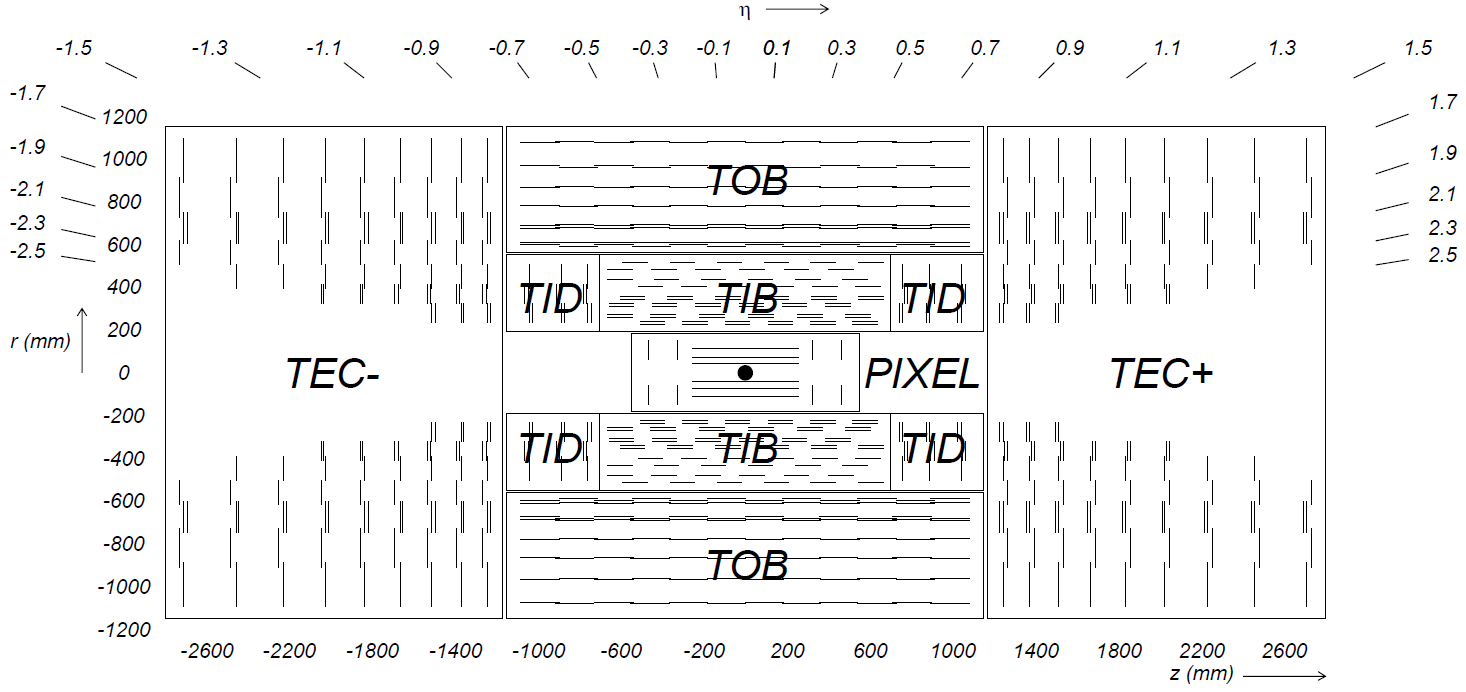
\includegraphics[width=0.9\textwidth]{Images/cmsTracker_TrackerLayout}
\caption{Schematic cross section through the CMS tracker in the $r-z$ plane: each line represents a detector module. Double lines indicate back-to-back modules which deliver stereo hits.}
\label{tracking_system}
\end{figure}
\begin{figure}[h!]
 \centering
 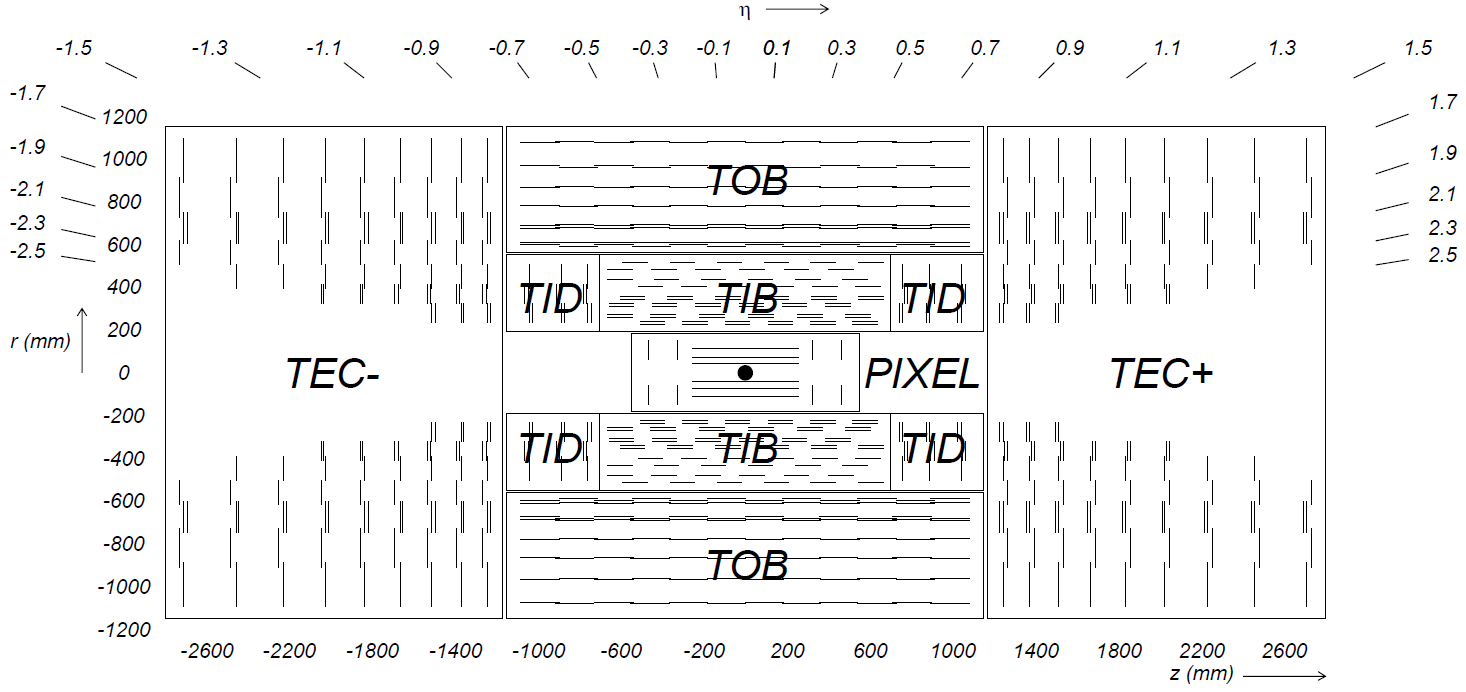
\includegraphics[width=0.1\textwidth]{Images/cmsTracker_TrackerLayout}
\caption{Material budget in units of radiation length as a function of pseudorapidity $\eta$ for the different sub-detectors (left panel) and broken down into the functional contributions (right panel).}
\label{Material_Budget}
\end{figure}
\begin{comment}
% PLOT DELLE PERFORMANCE DEL TRACKER PRESE DAL TDR DEL 2008 --> VANNO MESSE??? VANNO AGGIORNATE???
The tracker has a fundamental role in measuring kinematic variables of the particles: in \figurename~\ref{Tracker_performance_2} is shown the expected resolution of transverse momentum, transverse impact parameter and longitudinal impact parameter, as a function of pseudorapidity for single muons of transerve momentum of 1, 10 and 100 $GeV$. 
\begin{figure}[htbp]
\centering
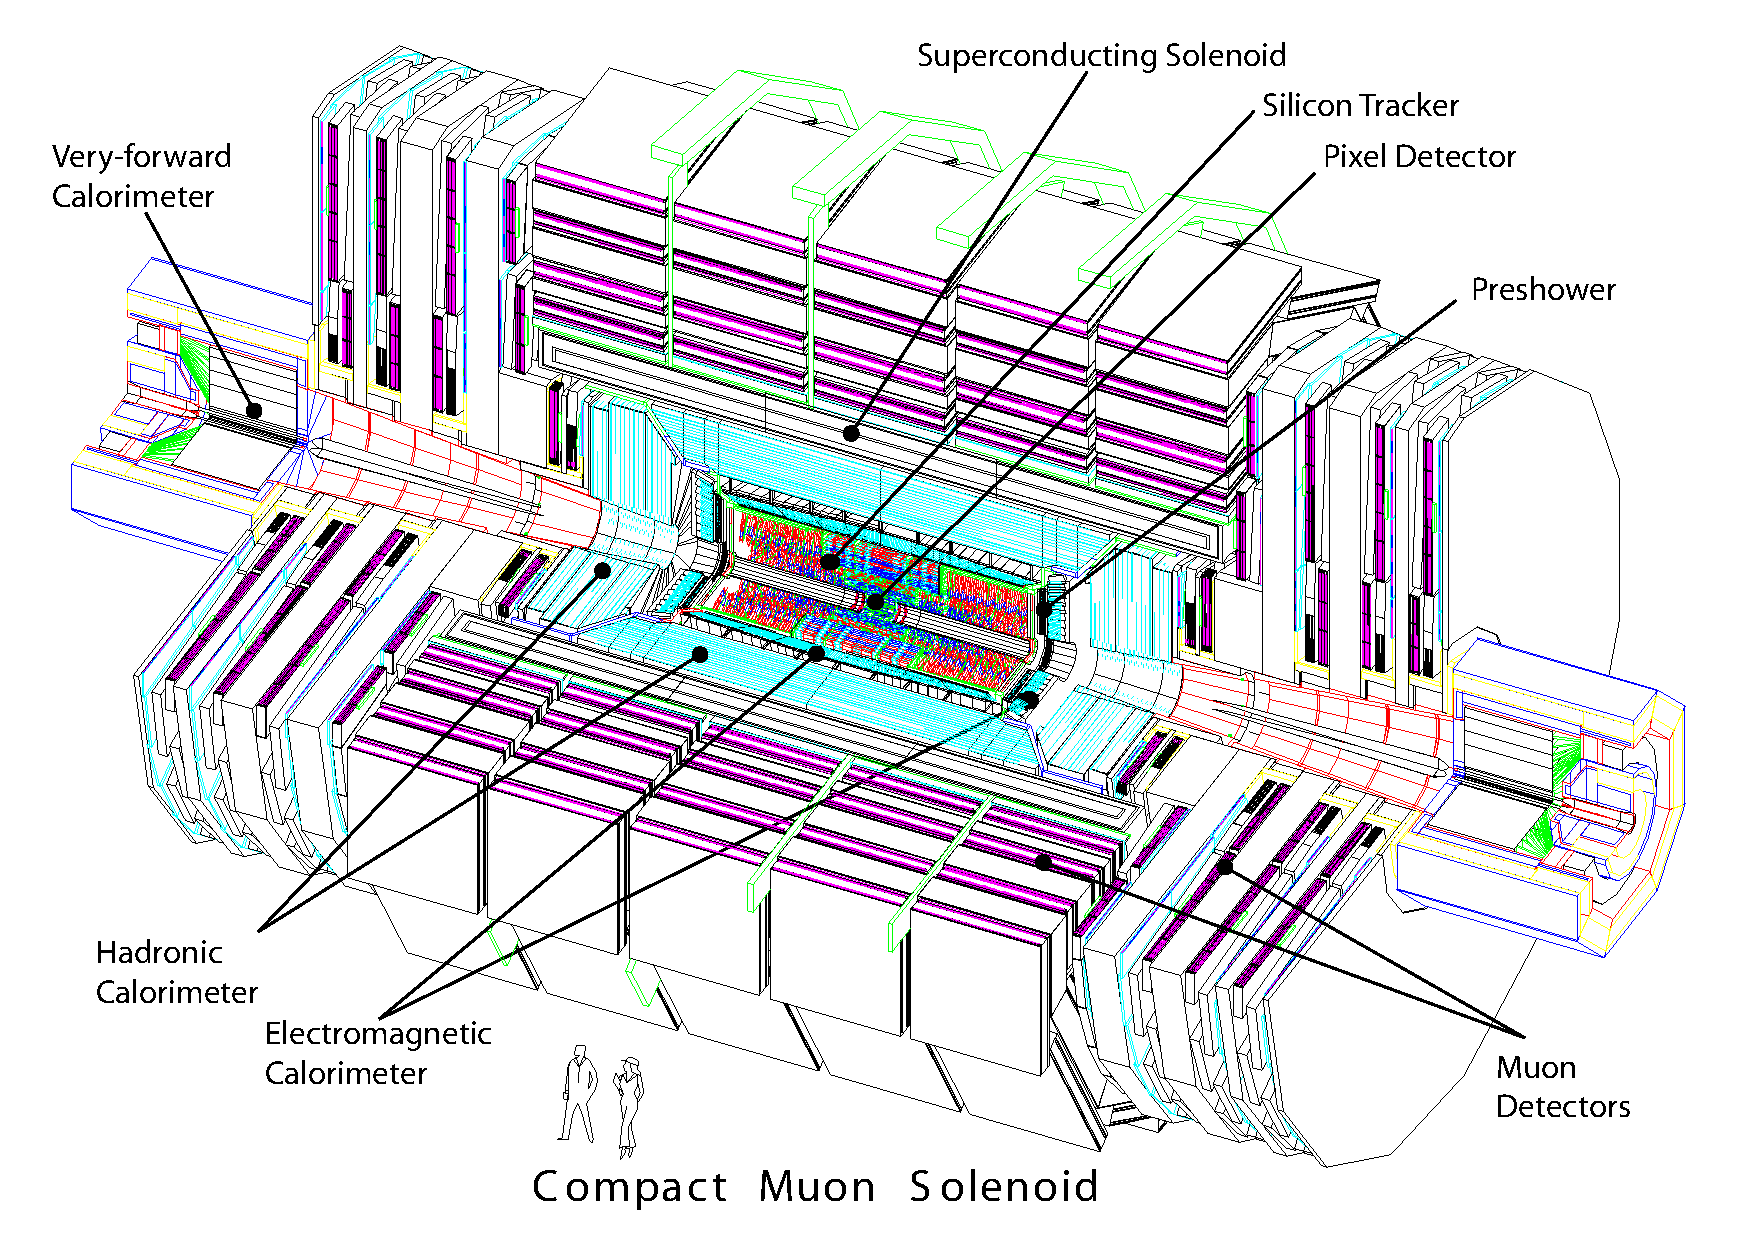
\includegraphics[width=0.1\textwidth]{Images/CMS_Layout.pdf}
\caption{Resolution for single muons with transverse momentum of 1, 10 and 100 GeV for several track parameters: transverse momentum (left panel), transverse impact parameter (middle panel), and longitudinal impact parameter (right panel).}
\label{Tracker_performance}
\end{figure}
For high momentum tracks (100 GeV) the transverse momentum resolution is around 1 - 2\% up to $|\eta| \approx 1.6$, beyond which it degrades due to the reduced lever arm. At a transverse momentum of 100 GeV multiple scattering in the tracker material accounts for 20 to 30\% of the transverse momentum resolution while at lower momentum it is dominated by multiple scattering. The transverse impact parameter resolution reaches 10 $\mu$m for high $p_{T}$ tracks, dominated by the resolution of the first pixel hit, while at lower momentum it is degraded by multiple scattering (similarly for the longitudinal impact parameter). \figurename~\ref{Tracker_performance}  shows the expected track reconstruction efficiency of the CMS tracker for single muons as a function of pseudorapidity: the efficiency is about 99\% over most of the acceptance and it decreases slightly at $|\eta| \approx 0$ due to gaps between the ladders of the pixel detector at z $\approx$ 0. At high $\eta$ the efficiency drop is mainly due to the reduced coverage by the pixel forward disks. \\ 
\begin{figure}[htbp]
\centering
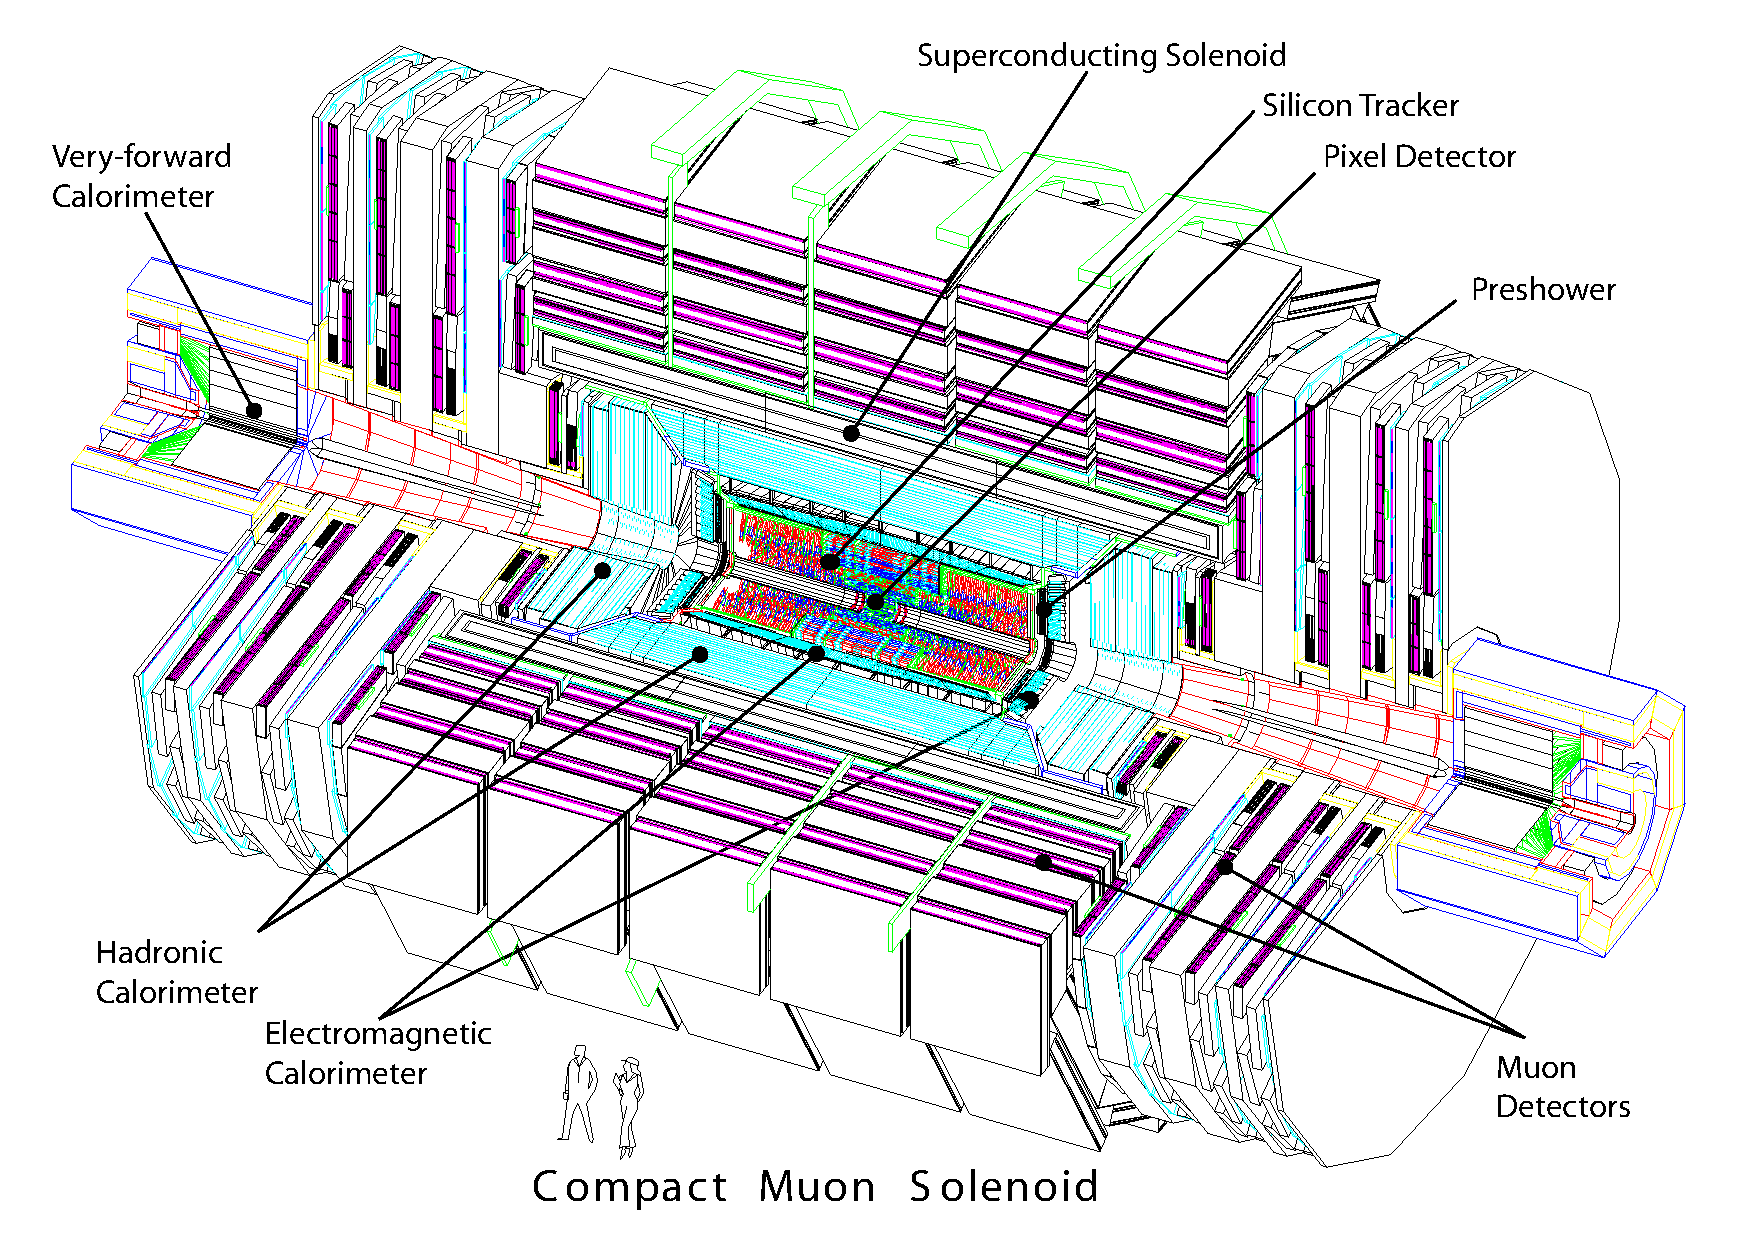
\includegraphics[width=0.1\textwidth]{Images/CMS_Layout.pdf}
\caption{Global track reconstruction efficiency for muons of several transverse momentum: 1, 10, 100 GeV.}
\label{Tracker_performance_2}
\end{figure}
% PLOT DELLE PERFORMANCE DEL TRACKER PRESE DAL TDR DEL 2008 --> VANNO MESSE??? VANNO AGGIORNATE???
\end{comment}

\subsubsection{The pixel detector}
The pixel system is the part of the tracking system that is closest to the interaction region and covers a pseudorapidity range $-2.5 < \eta  < 2.5$, matching the acceptance of the central tracker. \figurename~\ref{Pixel_structure} shows the geometric pixel strcture. It contributes precise tracking points in $r - \phi$ and z and therefore is responsible for a small impact parameter resolution that is important for good secondary vertex reconstruction. With a pixel cell size of $100 \times 150\ \mu m^{2}$ emphasis has been put on achieving similar track resolution in both $r-\phi$ and z directions: 10 $\mu m$ in $r - \phi$ direction and 20 $\mu m$ along z. The pixel detector is essential for the reconstruction of secondary vertices from b and tau decays, and forming seed tracks for the outer track reconstruction and high level triggering. It consists of three barrel layers (BPix) with two endcap disks (FPix). The 53-cm-long BPix layers will be located at mean radii of 4.4, 7.3 and 10.2 cm. The FPix disks, extending from $\approx$ 6 to 15 cm in radius, will be placed on each side at z=$\pm$34.5 and z=$\pm$46.5 cm. BPix (FPix) contain 48 million (18 million) pixels covering a total area of 0.78 (0.28) $m^{2}$. The arrangement of the 3 barrel layers and the forward pixel disks on each side gives 3 tracking points over almost the full $\eta$ range. In the high $\eta$ region the 2 disk points are combined with the lowest possible radius point from the 4.4 cm barrel layer.
\begin{figure}[htbp]
\centering
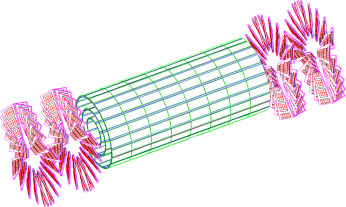
\includegraphics[width=0.5\textwidth]{Images/Pixel_structure}
\caption{Geometrical layout of the pixel detector.}
\label{Pixel_structure}
\end{figure}

\subsubsection{Pixel Upgrade}
Due to the radiation damage and significant data losses due to high occupancy in the readout chip of the pixel detector, the pixel system has been replaced by a new one in the end-of-year shutdown during winter 2016/2017 in order to maintain the excellent tracking and other physics performances \cite{New_Pixel_Detector}. The main new features of the upgraded pixel detector are a ultra-light mechanical design with four barrel layers and three end-cap disks, digital readout chip with higher rate capability and a new cooling system.
\begin{figure}[htbp]
\centering
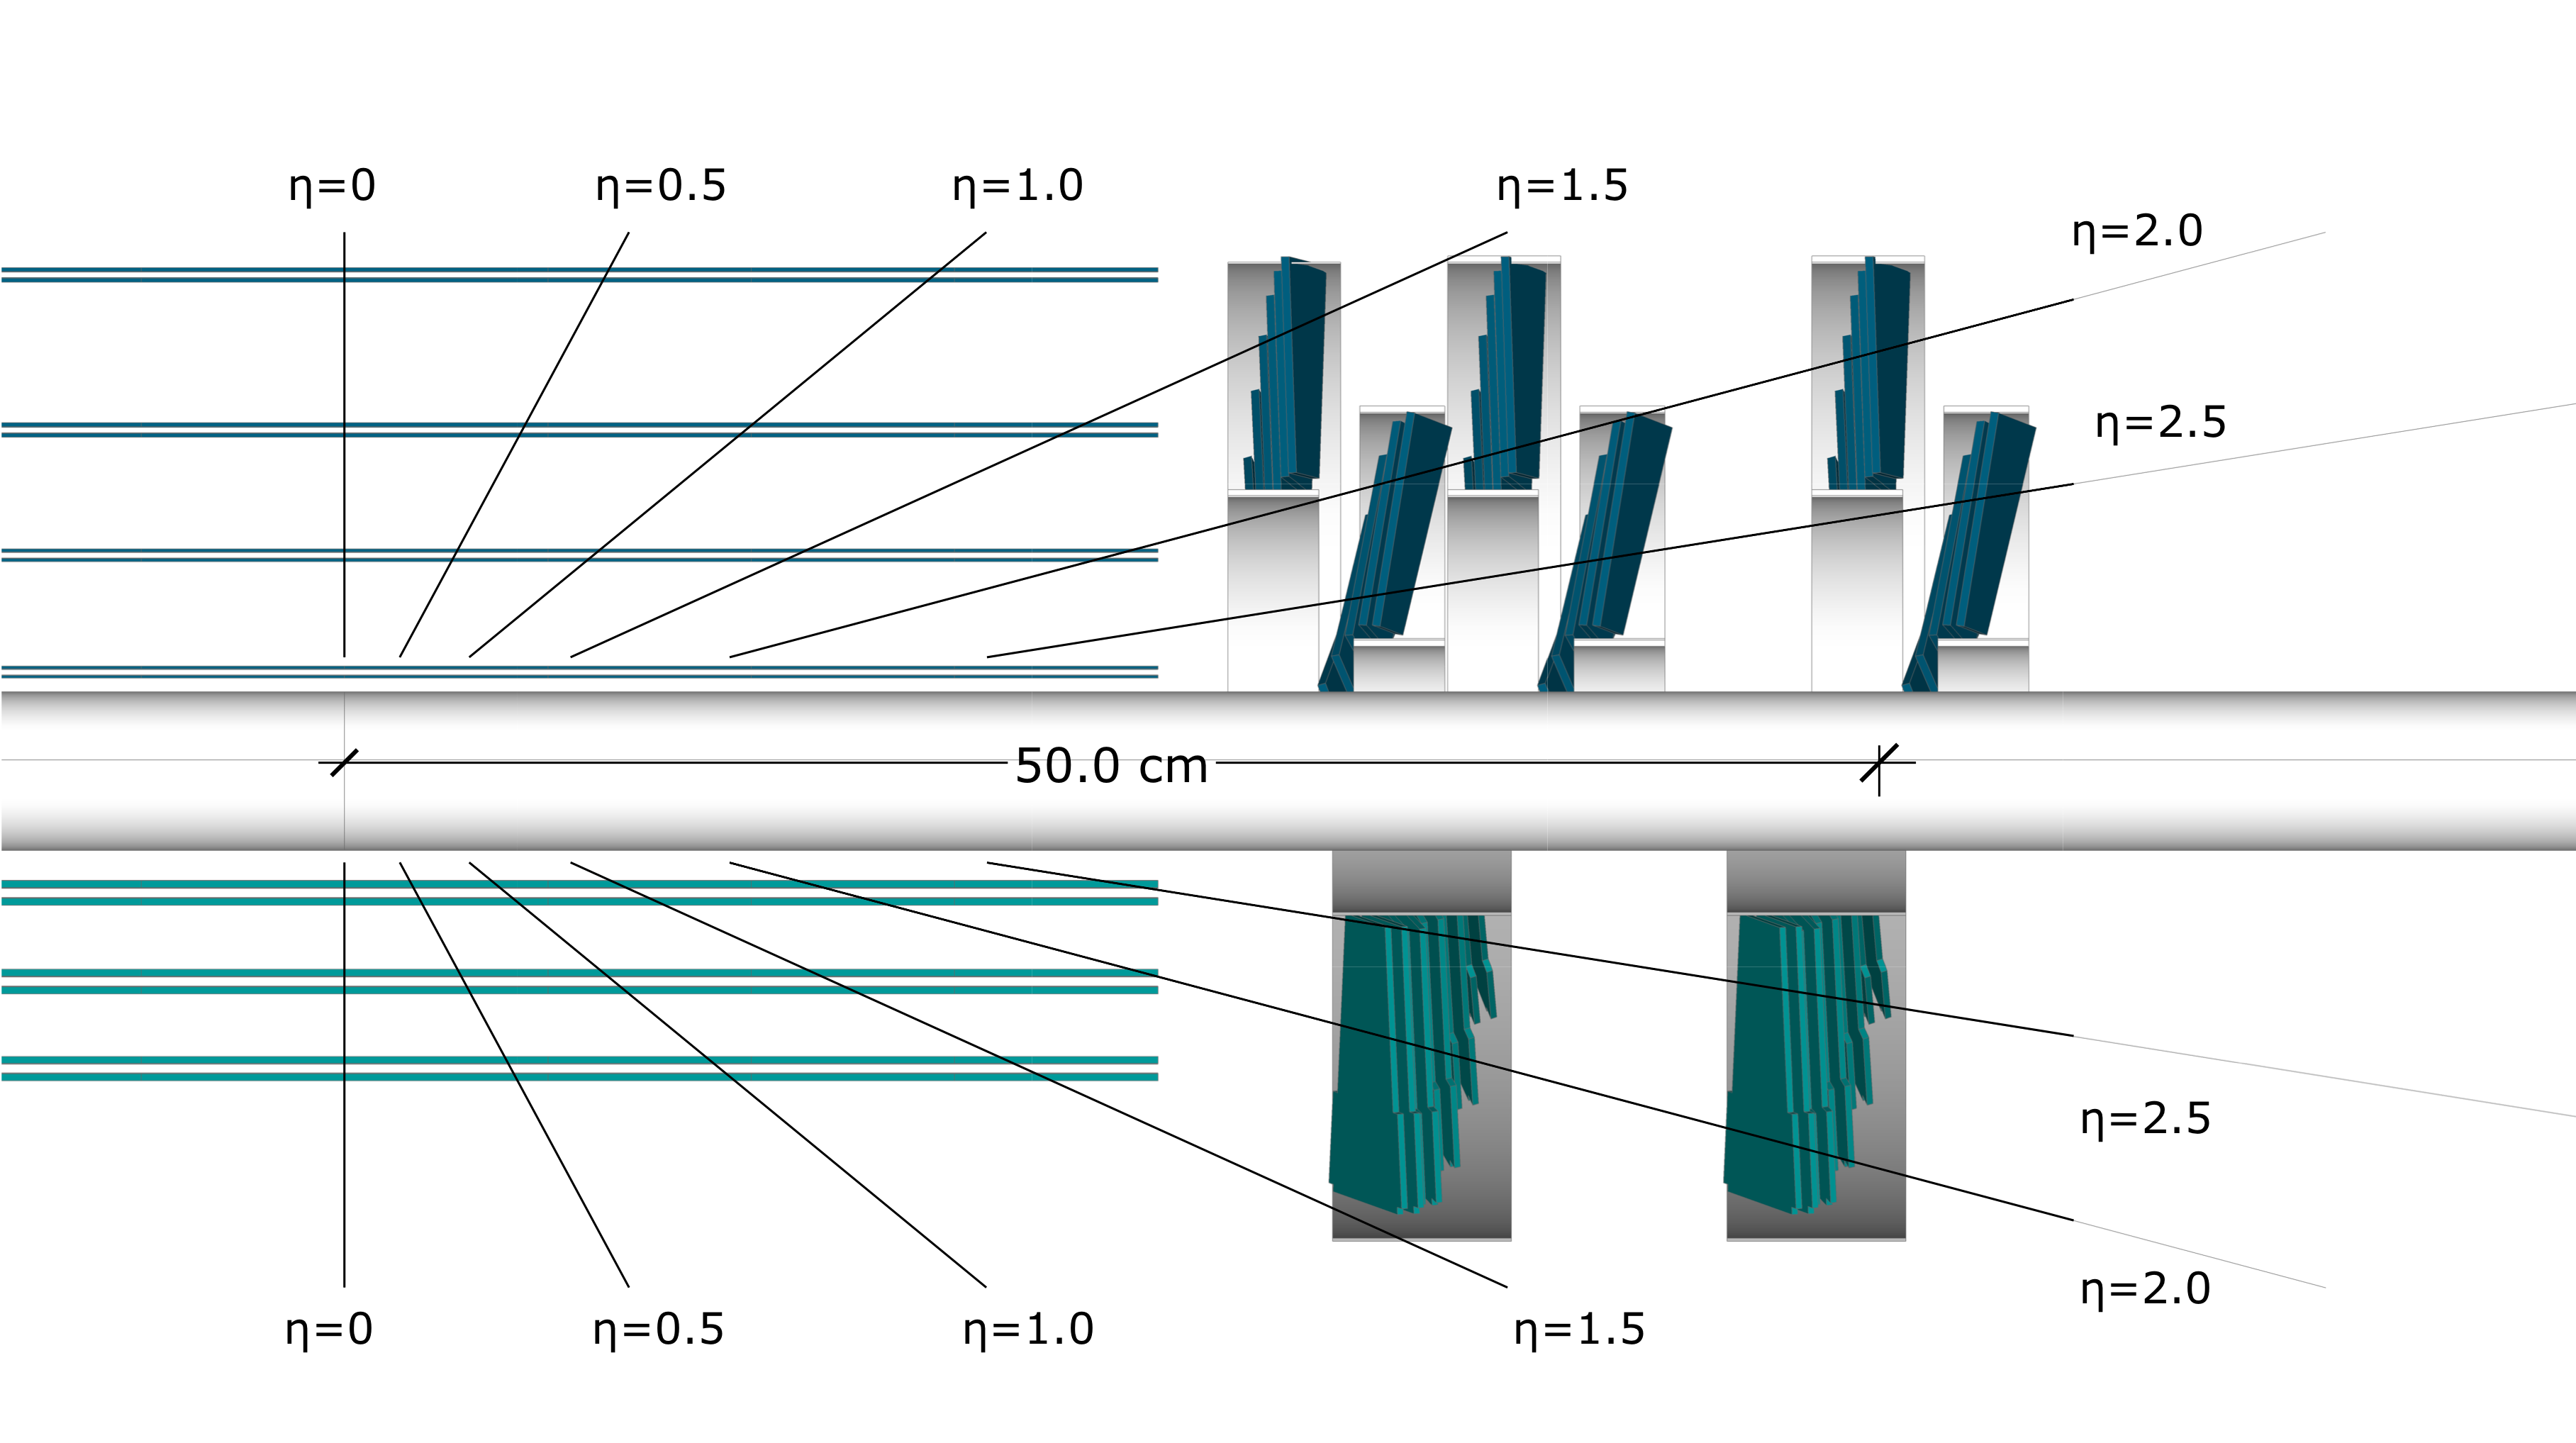
\includegraphics[width=0.65\textwidth]{Images/New_Pixel}
\caption{Comparison of the geometrical layouts of the old (bottom) and upgraded (top) CMS pixel detectors.}
\label{New_Pixel}
\end{figure}
The geometrical layout of the upgrade system, shown in \figurename~\ref{New_Pixel},  consists of four cylindrical barrel layers placed at radii of 29, 68, 109, 160 mm and three disks in each of the forward regions placed at a distance from the nominal interaction point of 291, 396 and 516 mm. This layout is optimized in order to offer full 4-hit tracking coverage up to pseudorapidities of 2.5, with an increased redundancy compared to the present system.

\subsubsection{The silicon strip detector}
The silicon strip detector is composed of three different subsystem. The Tracker Inner Barrel and Disks (TIB/TID  see \figurename~\ref{tracking_system}) are composed of 4 barrel layers, supplemented by 3 disks at each end. TIB/TID delivers up to 4 $r-\phi$ measurements on a trajectory using 320 $\mu m$ thick silicon microstrip sensors with their strips parallel to the beam axis in the barrel and radial on the disks. The strip pitch is 80$\mu m$ on layers 1 and 2 and 120 $\mu m$ on layers 3 and 4 in the TIB, leading to a single point resolution of 23 $\mu m$ and 35 $\mu m$, respectively. In the TID the mean pitch varies between 100$\mu m$ and 141$\mu m$. The TIB/TID is surrounded by the Tracker Outer Barrel (TOB). It has an outer radius of 116 cm and consists of 6 barrel layers of 500$\mu m$ thick microstrip sensors with strip pitches of 183$\mu m$ on the first 4 layers and 122$\mu m$ on layers 5 and 6. It provides another 6 $r-\phi$ measurements with single point resolution of 53$\mu m$ and 35$\mu m$, respectively. The TOB extends in z between $\pm$118cm. Beyond this z range the Tracker EndCaps ($\pm$TEC, where the sign indicates the location along the z axis) cover the region 124 cm $< |z| <$ 282 cm and 22.5 cm $< |r| < $113.5 cm. Each TEC is composed of 9 disks, carrying up to 7 rings of silicon microstrip detectors (320$\mu m$ thick on the inner 4 rings, 500$\mu m$ thick on rings 5-7) with radial strips of 97$\mu m$ to 184$\mu m$ average pitch. Thus, they provide up to 9 $\phi$ measurements per trajectory. In addition, the modules in the first two layers and rings, respectively, of TIB, TID, and TOB as well as rings 1, 2, and 5 of the TECs carry a second microstrip detector module which is mounted back-to-back with a stereo angle of 100 mrad in order to provide a measurement of the second coordinate (z in the barrel and r on the disks). The achieved single point resolution of this measurement is 230$\mu m$ and 530$\mu m$ in TIB and TOB, respectively, and varies with pitch in TID and TEC. \\
The sensor elements in the strip tracker are single sided p-on-n type silicon micro-strip sensors shown in \figurename~\ref{Silicon_structure}: in TIB/TID and on the inner 4 rings of the TECs, thin sensors of (320 $\pm$ 20) $\mu m$ wafer thickness are used, with substrate resistivity of $ro$ = 1.55 - 3.25 k$\Omega$cm; TOB and the outer 3 rings of the TECs are equipped with thicker sensors of (500 $\pm$ 20) $\mu m$ thickness, with substrate resistivity of $ro$ = 4 - 8 k$\Omega$cm. 
\begin{figure}[htbp]
\centering
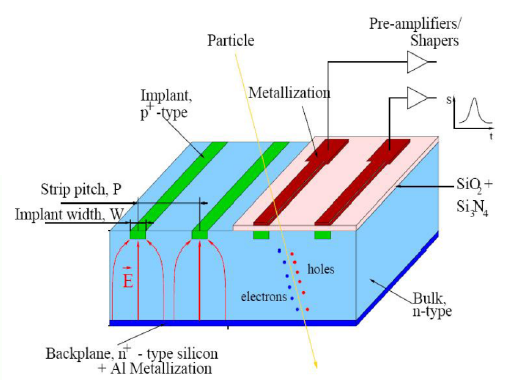
\includegraphics[width=0.35\textwidth]{Images/Silicon_structure}
\caption{Single sided p-on-n type silicon micro-strip sensor.}
\label{Silicon_structure}
\end{figure}

LASER ALIGNMENT SYSTEM

\subsection{Electromagnetic calorimeter}
The electromagnetic calorimeter plays an essential role in the study of the physics of electroweak symmetry breaking, and  in the exploration of  beyond the Standard Model scenarios.  ECAL is a homogeneous calorimeter of almost 76000 Lead Tungstate $PbWO_4$ scintillating crystals divided into a barrel and two endcaps.
A $3$D view of the barrel and endcap electromagnetic calorimeter is shown in \figurename~\ref{ECAL_3D}.
\begin{figure}[h!]
 \centering
 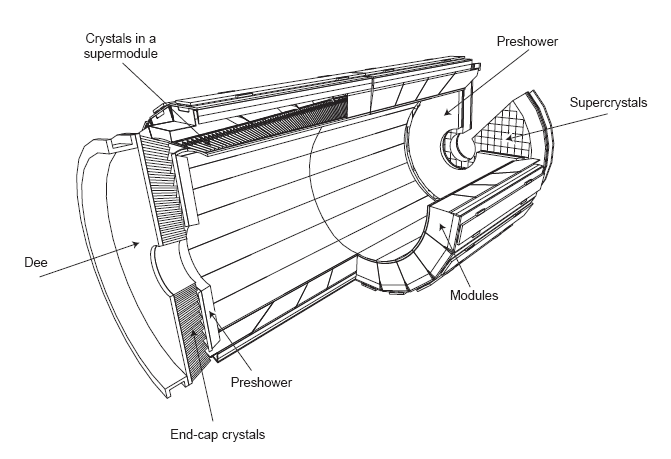
\includegraphics[width=0.75\textwidth]{Images/ECAL_3D}
 \caption{A $3$D view of the electromagnetic calorimeter.}
\label{ECAL_3D}
\end{figure}


\subsubsection{The Barrel Calorimeter}
The barrel part of the ECAL covers the pseudorapidity range $|\eta| < 1.479$ 
%(see Figure~\ref{fig:ecalSection}). 
The front face of the crystals is at a radius of $1.29 \,$m and each crystal has a square cross-section of $ 22 \times 22 \,$mm$^2$ and a length of $230 \,$mm corresponding to $25.8 \,$X$_0$. The truncated pyramid-shaped crystals are mounted in a geometry which is off-pointing with respect to the mean position of the primary interaction vertex, with a $3^{\circ}$ tilt in both $\phi$ and in $\eta$. The crystal cross-section corresponds to $\Delta \eta \times \Delta \phi = 0.0175 \times 0.0175$ ($1^{\circ}$). 
\begin{comment}
\begin{figure}[h!]
 \centering
 \includegraphics[width=0.80\textwidth]{cms/img/ecalTDR/longitudinal-view-16.pdf}
 \caption[ECAL longitudinal section]{Longitudinal section of the electromagnetic calorimeter (one quadrant)}
\label{fig:ecalSection}
\end{figure}
\end{comment}
The barrel granularity is $360$-fold in $\phi$ and ($2 \times 85$)-fold in $\eta$, resulting in a total number of $61\,200$ crystals. The crystal volume in the barrel amounts to $8.14 \,$m$^3$ ($67.4 \,$t). Crystals for each half-barrel are grouped in $18$ supermodules each subtending $20^{\circ}$ in $\phi$. Each supermodule comprises four modules with $500$ crystals in the first module and $400$ crystals in each of the remaining three modules. For simplicity of construction and assembly, crystals have been grouped in arrays of $2 \times 5$ crystals which are contained in a very thin wall ($200 \,\mathrm{\mu m}$) alveolar structure and form a submodule.  Thermal regulation is carried out by two active systems: 1) a specially regulated cooling circuit which keeps the operating temperature (ambient temperature) of the crystal array and of the APDs within a tight temperature spread of $\pm0.05 \, ^{\circ}$C, ensuring adequate thermal stability; 2) the power cooling circuit evacuates the heat generated by all power sources in the supermodule (each supermodule is designed as a separate thermal entity).

\begin{comment}
\subsection{The Endcap Calorimeter}

The endcap part of the crystal calorimeter covers a pseudorapidity
range from $1.48$ to $3.0$. The design of the endcaps provides precision
energy measurement up to $|\eta| = 2.5$. Crystals are however installed
up to $|\eta| = 3$ in order to augment the energy-flow measurement in
the forward direction.  The mechanical design of the endcap calorimeter
is based on an off-pointing pseudo-projective geometry using tapered
crystals of the same shape and dimensions ($24.7 \times 24.7 \times 220 \,$mm$^3$)
grouped together into units of $36$, referred to as supercrystals. A
total of $268$ identical supercrystals is used to cover each
endcap with a further $64$ sectioned supercrystals used to complete
the inner and outer perimeter. Each endcap contains 7324 crystals,
corresponding to a volume of $1.52 \,$m$^3$ ($12.6 \,$t). Both endcaps are
identical. Each endcap detector is constructed using Dee-shaped
sections as seen in Figure~\ref{fig:EE}. 
\begin{figure}[h!]
 \centering
 \includegraphics[width=0.50\textwidth]{cms/img/ecalTDR/endcap-18.pdf}
 \caption{A single endcap with Dees apart.}
\label{fig:EE}
\end{figure}

Figure~\ref{fig:materialBudget} shows the total thickness (in radiation
lengths) of the ECAL as a function of pseudorapidity. The
endcap part also includes the preshower detector.  
\begin{figure}[h!]
 \centering
 \includegraphics[width=0.50\textwidth]{cms/img/ecalTDR/material-budget-17.pdf}
 \caption[ECAL thickness in X$_0$]{Total thickness in X$_0$ of the ECAL as a function of pseudorapidity, averaged over $\phi$.}
\label{fig:materialBudget}
\end{figure}
Because of the
high radiation levels in the endcaps all materials
used in this region must tolerate very large doses and neutron fluences.  



\subsection{The Preshower Detector} 

The endcap preshower covers a pseudorapidity range
from $|\eta| = 1.65$ to $2.61$. 
Its main function is to provide $\pi^{0}$-$\gamma$ separation. 
The preshower detector, placed
in front of the crystals, contains two lead converters of a total
thickness of $2 \,$X$_0$ and $1 \,$X$_0$ respectively, followed by detector
planes of silicon strips with a pitch of $< 2 \,$mm. The impact position
of the electromagnetic shower is determined by the center-of-gravity
of the deposited energy. The accuracy is typically $300 \,\mathrm{\mu m}$ at 
$50 \,$ GeV. In order to correct for the energy deposited in the lead
converter, the energy measured in the silicon is used to apply
corrections to the energy measurement in the crystal. The fraction
of energy deposited in the preshower (typically $5\%$ at $20 \,$ GeV)
decreases with increasing incident energy.
Figure~\ref{fig:ES} shows the
layout of the preshower.
\begin{figure}[h!]
 \centering
 \includegraphics[width=0.80\textwidth]{cms/img/ecalTDR/es-19.pdf}
 \caption{Schematic section through the endcap preshower.}
\label{fig:ES}
\end{figure}

To maintain its performance during the lifetime of the experiment,
the endcap silicon detector has to be operated at $-5 \, ^{\circ}$C. Heating
films and insulating foam glued on the moderators guarantee that
the external surfaces are kept at the ambient temperature of the
neighboring detectors.


\subsection{Lead Tungstate Crystals}
The characteristics 
of the Lead Tungstate crystals (PbWO$_4$) make them an appropriate choice for operation at LHC~\cite{Beringer:1900zz}. The high density ($8.3 \,$g/cm$^3$), short radiation length ($0.89 \,$cm) and small
Moli\`ere radius ($2.2 \,$cm) results in a fine granularity and a compact
calorimeter. The scintillation decay time is of the same order of
magnitude as the LHC bunch crossing time: about $80\%$ of the light
is emitted in $25 \,$ns. The light output is relatively low: about $4.5$
photoelectrons per MeV are collected in both the avalanche photodiodes
(APDs) and the vacuum phototriodes (VPTs), where the higher APD
quantum efficiency is balanced by their smaller surface coverage
on the back face of the crystal. The crystals emit blue-green
scintillation light with a broad maximum at $420\,$nm~\cite{Annenkov:200230}. 


\subsection{Amplitude reconstruction}\label{sec:amplitude}
The raw data for a single channel consists of a series of consecutive digitization 
of the signal making up a time frame\cite{1748-0221-5-03-T03011}. The number of samples is adjustable (2+4n) with a default of 10. 
The digitizations are made at the bunch crossing frequency of 40 MHz, i.e. one sample each 25 ns.
 In addition, the timing of the signal is adjusted in LHC running so that the signal pulse maximum corresponds to one of the samplings. 
 Figure \ref{fig:ampl} shows an example of the time sampling for a signal pulse as a function of the time difference $(T-T_{max})$, 
 where $T$ and $T_{max}$ indicate the time of the generic ADC sample and the time corresponding to the maximum of the pulse shape respectively.
 \begin{figure}[h!]
 \centering
 \includegraphics[width=0.75\textwidth]{cms/img/ampl.png}
 \caption{Pulse shape measured in the ECAL as a function of $(T-T_{max})$.}
\label{fig:ampl}
\end{figure}
The simplest method of reconstructing the amplitude of the channel is to take the sampling on the maximum as
 the measurement of the signal. However, a larger number of samples is preferred since it allows more sophisticated digital 
 processing of the signal to reduce noise contribution. The other reason is to enable the identification of pile-up events from other bunch crossing.
The signal amplitude is computed as a linear combination of discrete time samples:
\begin{equation}
 A= \sum_{i=0}^N S_i \times w_i
 \end{equation}
where $w_i$ are the weights, $S_i$ the time sample values in ADC counts and $N$
  is the number of samples used in the filtering. The weights are determined to minimize the noise contribution.
Amplitude and time measurement are strongly correlated. After a signal has been amplified and shaped by the
   front-end electronics, the channel timing reconstruction consists in a precise measurement of the time the 
   pulse reaches its maximum values $A_{max}$. Looking at Figure \ref{fig:ampl}, the reconstructed time of a 
   channel corresponds to the value of $T_{max}$. 


\subsection{Energy Resolution}
For the energy range of
about $25$ GeV  to $500$ GeV, the ECAL energy resolution has been parameterized 
as: 
\begin{equation}
 \frac{\sigma(E)}{E} =  \frac{a}{\sqrt{E}} \oplus \frac{\sigma_n}{E} \oplus c \quad \text{(E in GeV)}
\end{equation}
 where $a$ is the
stochastic term, $\sigma_n$ the noise, and $c$ the constant term. 
Figure~\ref{fig:resolution-ecal} summarizes the different
contributions expected for the energy resolution. Terms representing
the degradation of the energy resolution at extremely high energies
have not been included. The stochastic
term includes fluctuations in the shower containment as well as a
contribution from photostatistics.  The noise term contains the contributions
from electronic noise and pile-up energy; the former is quite important
at low energy, the latter is negligible at low luminosity. The curve
labeled \textit{intrinsic} includes the shower containment and a constant
term of $0.55\%$. The constant term must be kept down to this level
in order to profit from the excellent stochastic term of PbWO$_4$ in
the energy range relevant for the search for new physics. To achieve this
goal, in situ calibration/monitoring using isolated high $p_T$ electrons
is performed.  
\begin{figure}[h!]
 \centering
 \includegraphics[width=0.85\textwidth]{cms/img/ecalTDR/resolution-13.pdf}
 \caption[Resolution of the PbWO$_4$ calorimeter]{Different contributions to the energy resolution of the PbWO$_4$ calorimeter.}
\label{fig:resolution-ecal}
\end{figure}

\subsection{ECAL Time measurement and resolution}
The algorithm used to extract $T_{max}$ relies on an alternative representation of the pulse shape, 
provided by a a variable defined as the ratio between the amplitudes of two consecutive samples\cite{1748-0221-5-03-T03011}:
\begin{equation}
R(T)=\frac{A(T)}{A(T+25ns)}
\end{equation}
where $A(T)$ represents the pulse amplitude at time $T$ . Figure \ref{fig:ration} illustrates the parametrization of time difference $(T-T_{max})$ as a function of $R(T)$.
 In view of the universal character of the pulse shape, this representation is independent on the maximum amplitude $A_{max}$
  and can be described well with a simple polynomial parametrization.
  \begin{figure}[h!]
 \centering
 \includegraphics[width=0.65\textwidth]{cms/img/ration.png}
 \caption{Time difference $(T-T_{max})$ as a function of the ratio of the amplitudes $R (T )$. }
\label{fig:ration}
\end{figure}

Each pair of consecutive samples gives a measurement of the ratio: 
 \begin{equation}
R_i=\frac{A(T+[i]\cdot 25ns)}{A(T+[i+1]\cdot25ns)}
\end{equation}
An estimate $T_{max,i}$ of the maximum time can be obtained from each $R_i$ ratio as $T_{max,i} = T_i-T (R_i)$. 
A more precise determination of the maximum time and its uncertainty is then obtained from the weighted average of the estimated $T_{max,i}$:
\begin{equation}
T_{max}=\frac{\sum_i \frac{T_{max,i}}{\sigma^2_i}}{\sum_i \frac{1}{\sigma^2_i}}
\end{equation}

\begin{equation}
\frac{1}{\sigma^2_T}=\sum_i \frac{1}{\sigma^2_i}
\end{equation}
The typical number of available ratios $R_i$ is five or six.

To determine the intrinsic time resolution of the ECAL, electrons from a test
beam with energy between 15 and 300 GeV are used.
 The time resolution is extracted from the distribution of the time difference
  between adjacent crystals that share the same electromagnetic shower and measure similar energies.
   The distribution of the time difference is well described by a Gaussian function, whose width can be parametrized as \cite{1748-0221-5-03-T03011}:
 \begin{equation}
\sigma^2(t_1-t_2) = \left ( \frac{N\sigma_n}{A_{eff}} \right)^2+C^2
\end{equation}  
where $A_{eff} = E_1E_2/\sqrt{E_{1}^2 + E_2^2}$, with $t_{1,2}$ and $E_{1,2}$
 corresponding to the times and energies measured in the two crystals, $\sigma_n$ is a parameter related to the noise level, 
 $N$ and $C$ represent the noise and constant term coefficients of time resolution. 
 The extracted width is presented in Figure \ref{fig:timereso} as a function of the variable $A_{eff}/\sigma_n$. 
 The energy scales for barrel and endcap are superimposed in the plot.
 \begin{figure}[h!]
 \centering
 \includegraphics[width=0.65\textwidth]{cms/img/timereso.png}
 \caption{ Gaussian width of the time difference between two neighboring crystals as a function of the variable $A_{eff}/\sigma_n$,
  for test beam electrons between 15 and 300 GeV. The equivalent single-crystal energy scales for barrel and endcaps are overlaid on the plot.}
\label{fig:timereso}
\end{figure}

Precise ECAL time determination results to be crucial in many respects.
The better the precision of time measurement and synchronization, 
the larger the rejection of backgrounds with a broad time distribution.
 Such backgrounds are cosmic rays, beam halo muons, electronic noise, and out-of- time proton-proton interactions.
  Precise time measurement also makes it possible to identify particles predicted by different models beyond the Standard Model. 
  Slow heavy charged R-hadrons \cite{Chatrchyan:2013oca}, which travel through the calorimeter and interact before decaying, 
  and photons from the decay of long-lived new particles that reach the calorimeter out-of-time with respect
   to particles travelling at the speed of light from the interaction point. To achieve these goals the time measurement performance both at low energy (1 GeV or less) and high energy (several tens of GeV) for showering photons have been studied also with collision data in order to reproduce the results obtained at the test beam.
    Indeed during collisions several effects can worsen significantly the design resolution, as for example, run by run variations, inter-calibration, effects vs energy, radiation, the presence of the  magnet field and of the tracker material in front of the ECAL. The time resolution estimated with 8 TeV data, looking at the time difference of electrons produced in the decay of a Z boson in CMS, is shown in Figure \ref{fig:timerescol}. The noise term results to be consistent with the one obtained at the test beam, while the constant term is about 150 ps. This value although far from the design performance, it is almost ok for every physics application.
An example of the use of the ECAL time measurement in physics analysis is presented in appendix \ref{app:neut}. In this analysis, for the first time, the novel technique of exploiting
 the ECAL time measurement is used to identify off time photons produced in the decays of long-lived neutralinos, with decay lengths comparable to the ECAL radial size.
  
   \begin{figure}[h!]
 \centering
 \includegraphics[width=0.65\textwidth]{cms/img/timerescol.png}
 \caption{ Gaussian width of the time difference between two electrons produced in the decay of a Z boson as a function of the variable $A_{eff}/\sigma_n$.
The equivalent single-crystal energy scales for barrel and endcaps are overlaid on the plot.}
\label{fig:timerescol}
\end{figure}

  
\section{Magnet}
The required performance of the muon system, and hence the bending power, is defined
by the narrow states decaying into muons and by the unambiguous determination of the
sign for muons with a momentum of $ 1\,$ TeV/c. This requires a momentum resolution of $\Delta p / p \sim 10 \%$ at $p = 1$ TeV. 

To achieve this goal, CMS chose a large superconducting solenoid, the parameters of which are given in table~\ref{tab:magnetParameters}. 

\begin{table}[h!]
\centering

 \begin{tabular}{ l  c }
\toprule
Parameter & Value \\
  \midrule
  Field & $3.8\,$T \\
  Inner bore & $5.9 \,$m \\
  Length & $12.9 \,$m \\
  Number of turns & $2168$ \\
  Current & $19.5 \,$kA \\
  Stored energy & $2.7 \,$GJ\\
  \bottomrule
 \end{tabular}
 \caption{Parameters of the CMS superconducting solenoid.}
\label{tab:magnetParameters}
\end{table}



%\begin{figure}[ht]
\begin{figure}[h!]
 \centering
 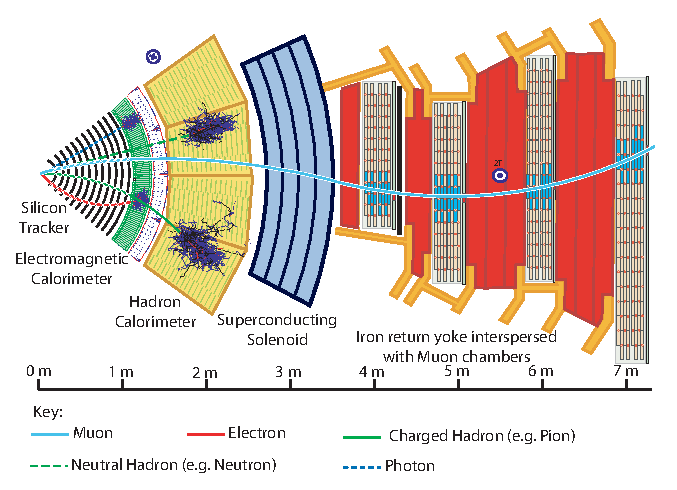
\includegraphics[width=0.85\textwidth]{cms/img/cms_slice.pdf}
 \caption{Schematic view of a transverse slice of the central part of the CMS detector.}
\label{fig:cmsSection}
%\end{figure}
\end{figure}
 



\section{Hadron Calorimeter}
\label{sec:HCAL}

The design of the hadron calorimeter (HCAL) \cite{CMS:1997tfa} is strongly influenced by the choice of the magnet parameters since most of the CMS calorimetry is located inside the magnet coil and surrounds the ECAL system (see figure~\ref{fig:cmsSection}). An important requirement of HCAL is to minimize
the non-Gaussian tails in the energy resolution and to provide good containment and hermeticity. Hence, the HCAL design maximizes material inside the magnet coil in terms of interaction lengths. This is complemented by an additional layer
of scintillators, referred to as the hadron outer (HO) detector, lining the outside of the coil.
Brass has been chosen as absorber material as it has a reasonably short interaction length,
is easy to machine and is non-magnetic. Maximizing the amount of absorber before the magnet requires minimizing the amount of space devoted to the active medium. The tile/fiber technology makes for an ideal choice. It consists of plastic scintillator tiles read
out with embedded wavelength-shifting (WLS) fibers. The WLS fibers are spliced to high-attenuation-length clear fibers are just outside the scintillator carrying the light to the readout system. 
The photodetection
readout is based on multi-channel hybrid photodiodes (HPDs). The absorber structure is assembled by bolting together precisely machined and overlapping brass plates so as to leave space to insert the scintillator plates, which have a thickness of $3.7 \,$mm. The overall assembly
enables the HCAL to be built with essentially no uninstrumented cracks or dead areas in $\phi$.
%The gap between the barrel and the endcap HCAL, through which the services of the ECAL
%and the inner tracker pass, is inclined at $53^{\circ}$ and points away from the center of the detector.


\section{Muon System}
The muon system is the outermost of the CMS subdetectors. Its main goals are the identification of muons, thanks to their high penetrating power, and
a precise measurement of their momentum, with the help of the information
coming from the tracker. The muon system also works as trigger for events
which involve muons and it provides a precise time measurement of the bunch
crossing.
The CMS muon system \cite{muon} relies on three kinds of gaseous detectors:
drift tubes (DT), cathode strip chambers (CSC) and resistive plate chambers
(RPC). The DT and the CSC provide an excellent spatial resolution for the measurement of charged particle momentum; the RPC are
used for trigger issues because of the very good timing. The active parts of
the muon system are hosted into stations which are interleaved by the iron
layers of the return yoke of the magnet. The longitudinal view of a quarter of
the muon system is given in Figure \ref{fig:muon}. The barrel extends up to $|\eta|<1.4$,
the endcaps up to $|\eta|<2.4$. 
\begin{figure}[h!]
 \centering
 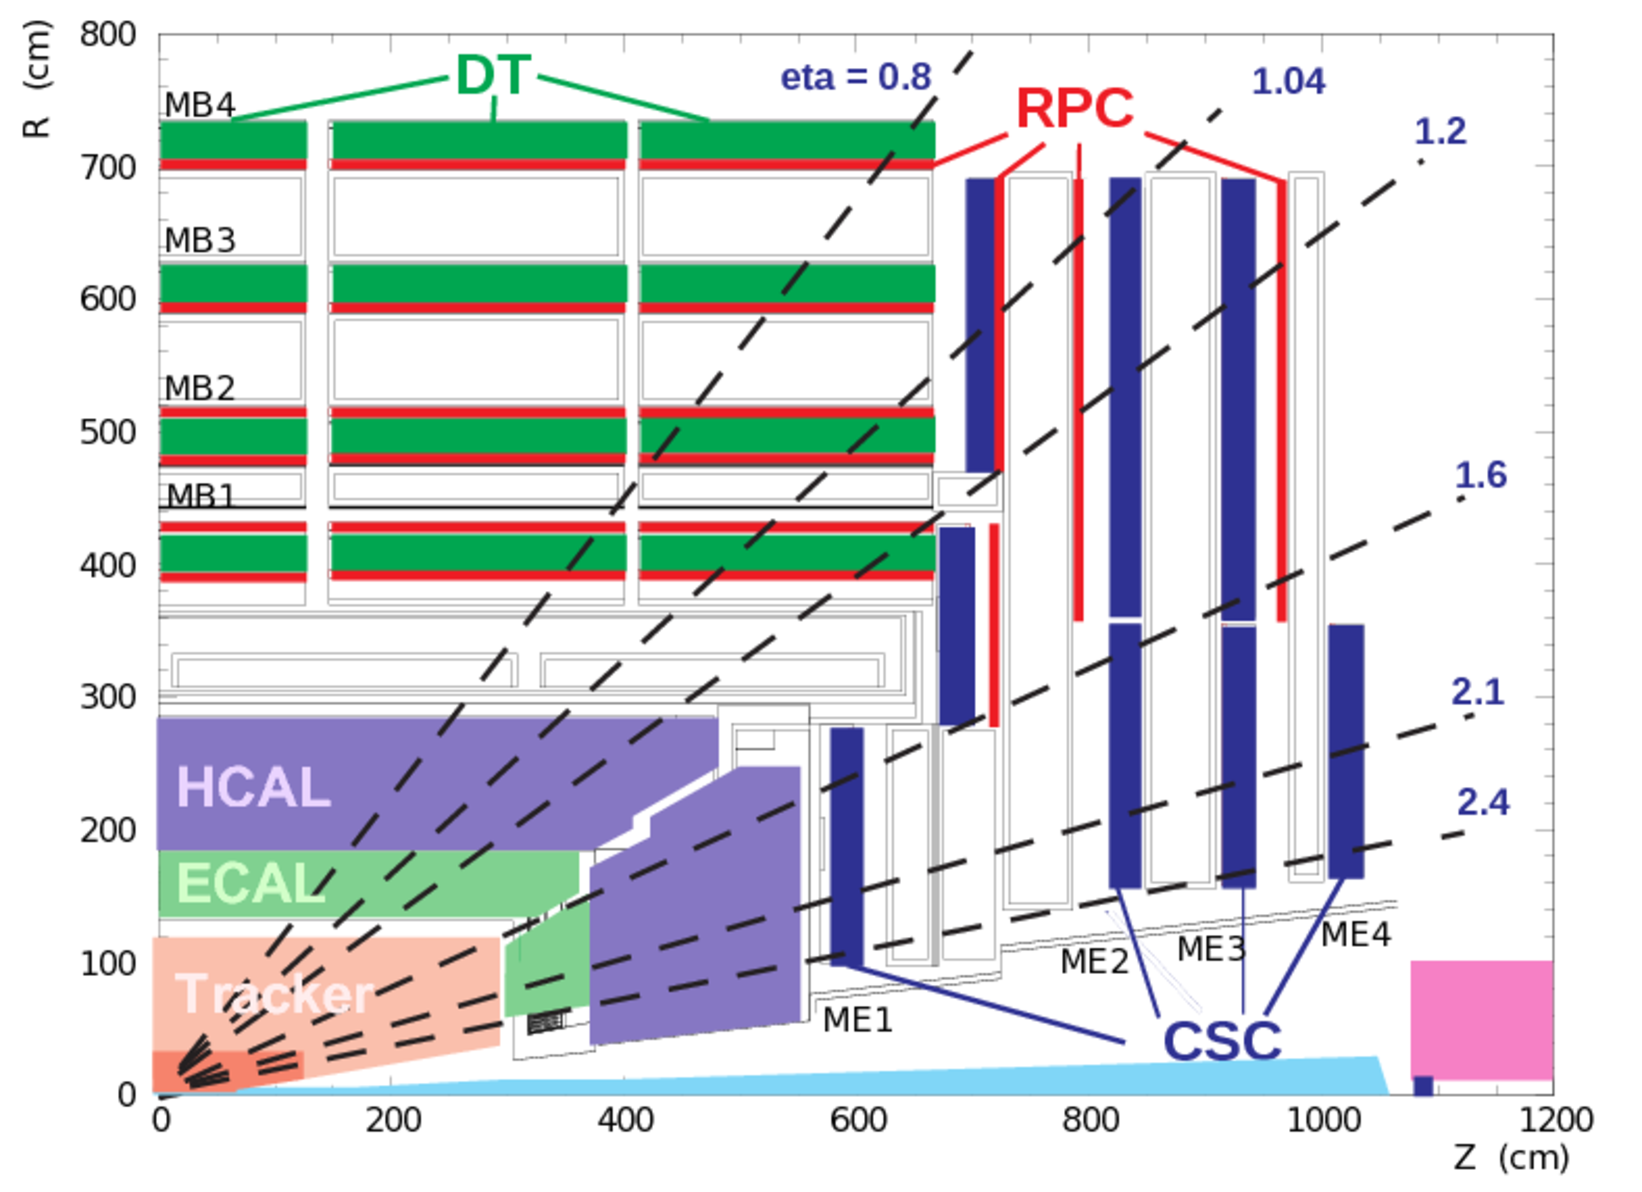
\includegraphics[width=0.85\textwidth]{cms/img/muonsyst.pdf}
 \caption{Longitudinal view of one quarter of the CMS muon system}
\label{fig:muon}
%\end{figure}
\end{figure}
 

\section{Trigger and Data Acquisition}\label{sec:trig}

The trigger system in CMS is the start of the physics event selection process. A
decision to retain an event for further consideration has to be
made every $25 \,$ns. This decision is based on the event's suitability
for inclusion in one of the various datasets to be used for analysis.
The datasets to be taken are determined by CMS physics priorities
as a whole. These datasets include dilepton and multilepton datasets, diphoton datasets,
lepton plus jet datasets for top, Higgs and BSM physics, and inclusive electron datasets for calorimeter calibrations.
In addition, other samples are necessary for measuring efficiencies
in event selection and studying backgrounds. The trigger has to
select these samples in real time along with the main data samples.

For the nominal LHC design luminosity of $10^{34} \,$cm$^{-2}$s$^{-1}$, an average
of $17$ events occurs at the beam crossing frequency of $25$ ns. This
input rate of $10^9$ interactions every second must be reduced by a
factor of at least $10^7$ to $100 \,$Hz, the maximum rate that can be
archived by the on-line computer farm. CMS has chosen to reduce
this rate in two steps. At the first level (L1) all data is stored for
$3.2 \, \mathrm{\mu s}$, after which no more than $100 $\,kHz of the stored events are
forwarded to the High Level Triggers (HLT). The L$1$ system uses only coarsely segmented
data from calorimeter and muon detectors, while holding all the
high-resolution data in pipeline memories in the front-end electronics.
The HLT is provided by a subset of the on-line processor farm which,
in turn, passes a fraction of these events to the remainder of the
on-line farm for more complete processing.





\subsection{Level $1$ Trigger}

The design of the CMS Trigger and Data Acquisition system is illustrated in figure~\ref{fig:trigger}.
\begin{figure}[h!]
\centering
 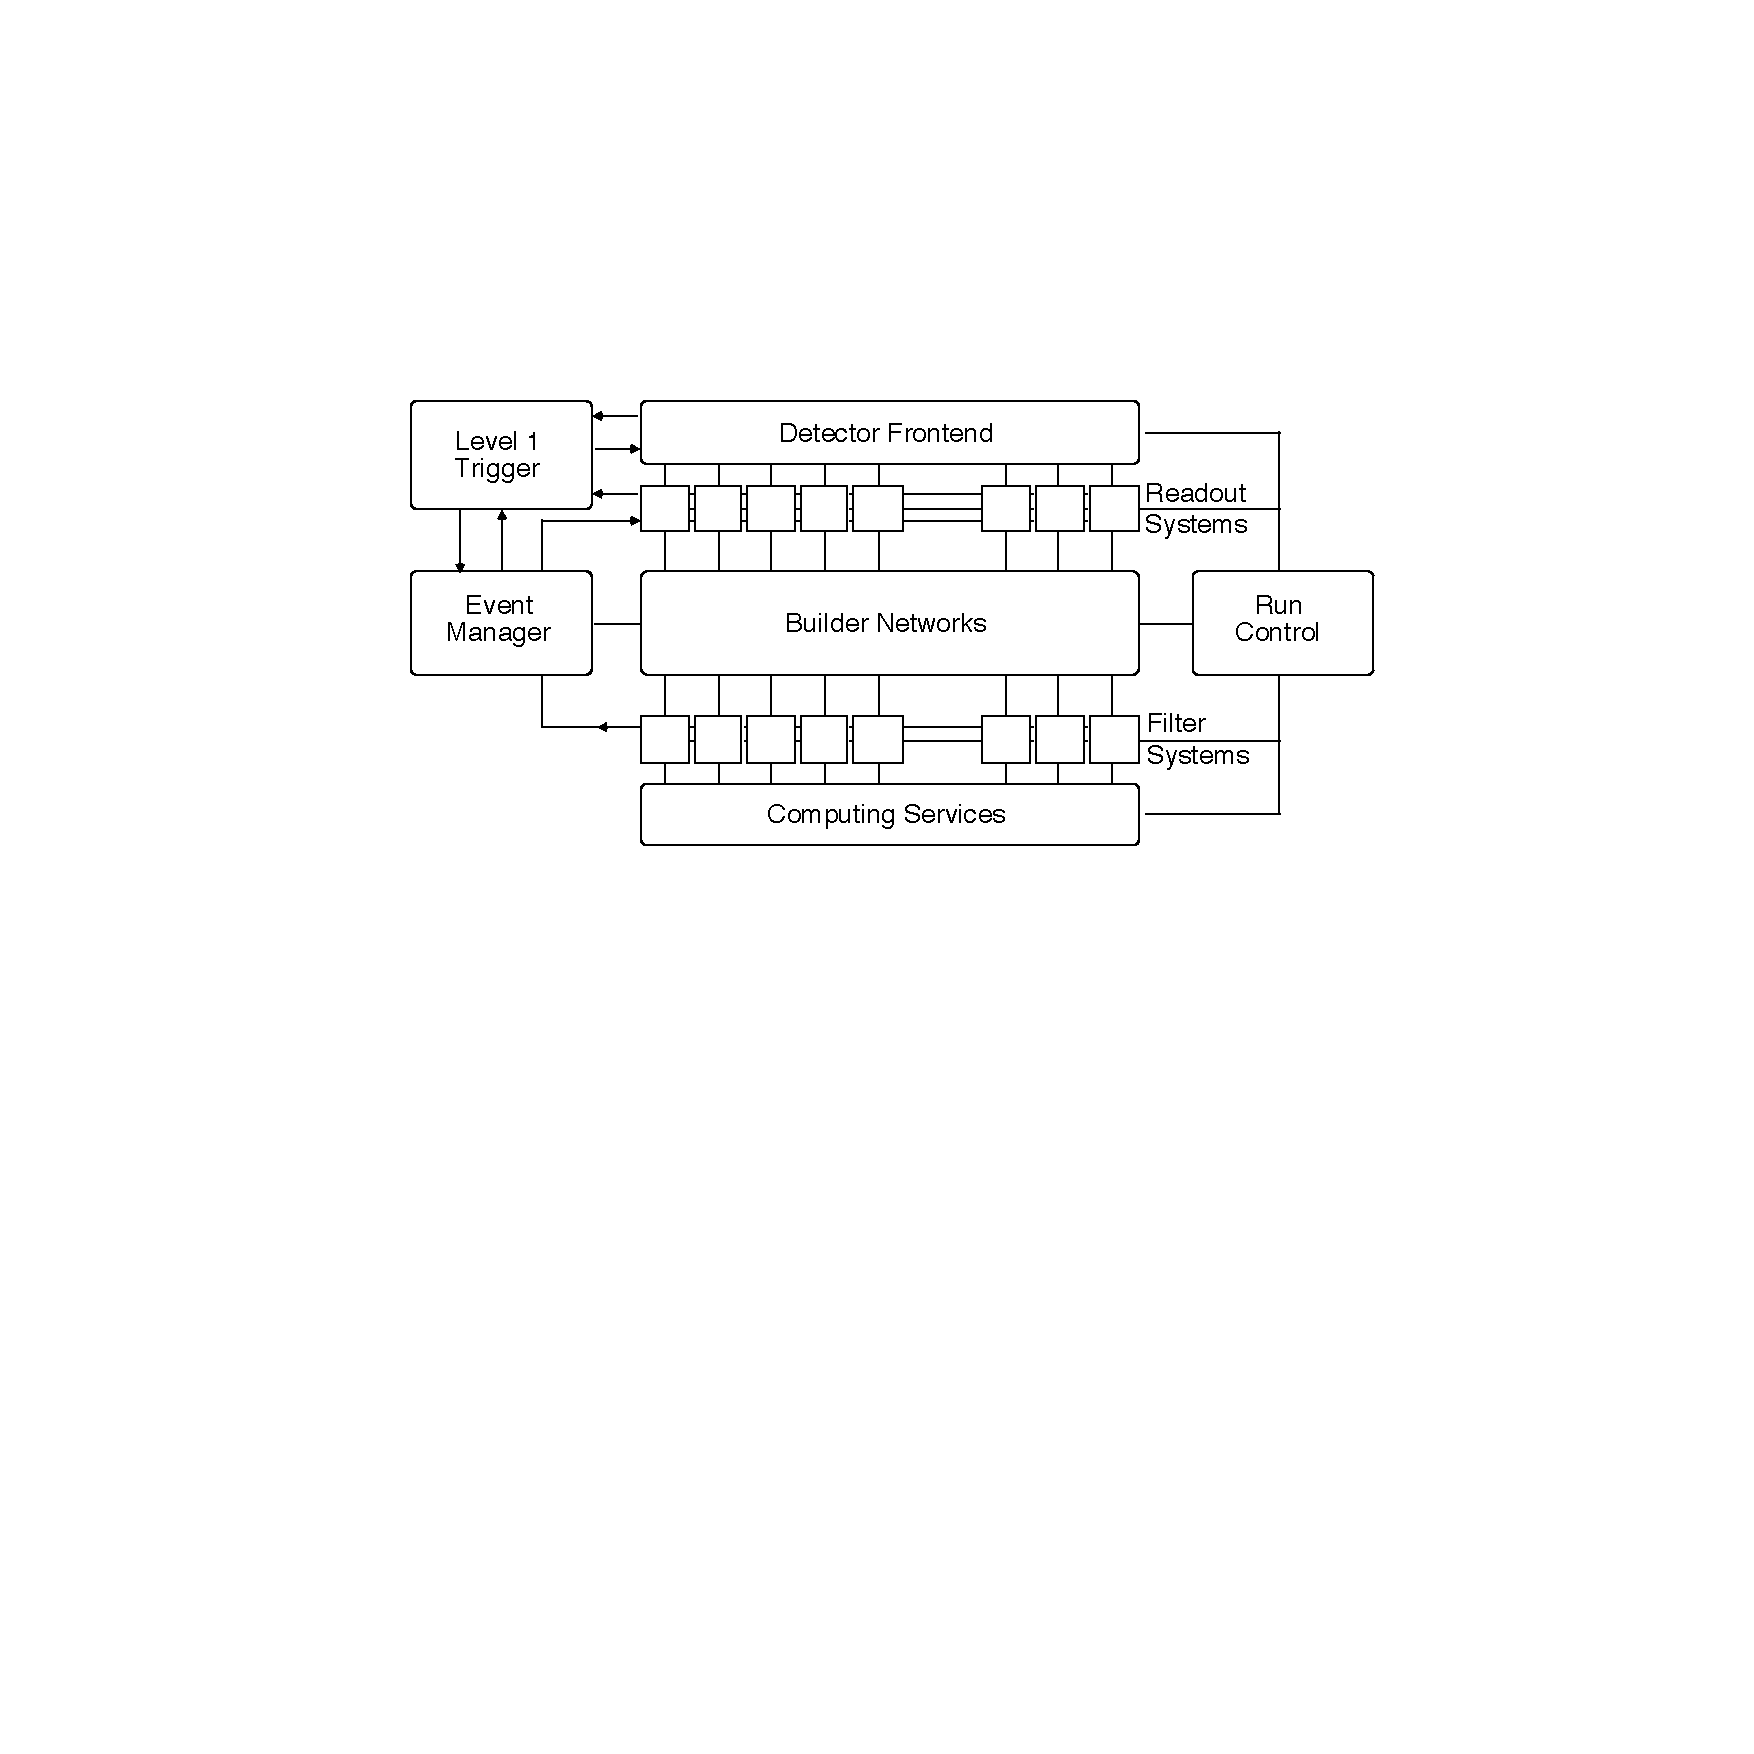
\includegraphics[width=0.9\textwidth]{cms/img/trigger}
\caption{CMS Trigger and Data Acquisition System.}
\label{fig:trigger}
\end{figure}
At the first level all information about the event is preserved.
The first level decision is made, with negligible dead-time, on a
subset of the total information available for the events. Since signal propagation delays are included in
this pipeline time, the L$1$ trigger calculations must be done in
many cases in less than $1 \, \mathrm{\mu s}$. If the first level trigger generates
an accept, the event data are moved or assigned to a buffer for
readout and processing by the High Level Triggers.



The L$1$ trigger involves the calorimetry and muon systems as well
as some correlation of information from these systems. The L$1$
decision is based on the presence of local objects such as photons,
electrons, muons, and jets, using information from calorimeters,
and muon systems in a given element of $\eta$-$\phi$ space. It also employs
global sums of $E_T$ and missing $E_T$. Each of these items is tested
against several $p_T$ or $E_T$ thresholds.


\subsection{High Level Trigger}

The CMS Level-$1$ Trigger System is required to reduce the input
interaction rate of $1 \,$GHz to a filtered event rate of $75 \,$kHz. 
To match the capabilities of the mass storage and offline computing systems, the final output of the
experiment should not exceed $100$ events per second.


The High Level Triggers have access to all the information used in
L$1$ since this is stored locally in the L$1$ trigger crates. Consequently,
High Level Triggers can make further combinations and other topological
calculations on the digital list of objects transmitted from L$1$.
Eventually, the High Level Triggers use the full event data for the decision
to keep an event.
\end{comment}




\selectlanguage{english}
\chapter{Il Modello Standard e la Fisica del Bosone di Higgs}
\label{Chapter1}
%SourceDoc tesi.tex

La fisica delle particelle elementari � una branca della fisica che si occupa dello studio dei costituenti elemetari della materia e delle loro interazioni fondamentali. I vari risultati ottenuti negli ultimi 50 anni di esperimenti portano al successo un unico modello teorico: il Modello Standard (MS) dell'interazioni elettrodeboli e forti delle particelle fondamentali. \\




\selectlanguage{english}
\chapter{Search for SM Higgs}
\label{Chapter4}

The analysis presented in this chapter consists in the search for the Standard Model Higgs with a mass of 125 GeV decaying into two muons.  \\






\chapter*{Conclusion}
\addcontentsline{toc}{chapter}{Conclusion}
\pagestyle{plain}

In questo lavoro di tesi ho analizzato il processo di produzione associata, nell'ambito dell'esperimento CMS a LHC, per $m_H=$125 GeV. Lo stato finale analizzato � il seguente:
\[ (W\rightarrow \mu+\nu_{\mu})(H\rightarrow \tau^+ \tau^- \rightarrow \tau_{jet} + \tau _{jet} + 2\nu_{\tau}),\]



\addcontentsline{toc}{chapter}{Bibliography}
\begin{thebibliography}{999}

% stile: Autori (normale): titolo (corsivo), data (normale). Sito web (normale)
      % \bibitem[]{} \textbf{}: \emph{}, .
%______________________________________________________________________________
				%cap1
		\bibitem{PDG} C. Patrignani et al. (Particle Data Group), Chin. Phys. C, 40, 100001 (2016) and 2017 update.
		\bibitem{HalzenMartin} Halzen and Martin, \emph{Quarks and Leptons: An Introductory Course in Modern Particle Physics}, John Wiley \& Sons (1984).
		\bibitem{Peskin} M.E.Peskin and D.V.Schroeder, \emph{An Introduction To Quantum Field Theory}, Addison-Wesley, 1995.
		\bibitem{Maggiore} M.Maggiore, \emph{A Modern Introduction to Quantum Filed Theory}, Oxford University Press, 2004.
		\bibitem{QCD} A.Pich, \emph{The standard model of electroweak interactions}, arXiv:hep-ph/0502010v,  2005.
		\bibitem{Wboson}  UA1 Collaboration, \emph{Experimental observation of isolated large transverse energy electrons with associated missing energy at $sqrt{s}=540~GeV$.}
		\bibitem{Zboson} UA1 Collaboration, \emph{Experimental observation of lepton pairs of invariant mass around $95~GeV/c^{2}$ at the CERN SPS collider.}
		\bibitem{SU2_Hmechanism} S. Weinberg, \emph{A model of leptons}, Phys. Rev. Lett. 19 (1967) 1264.
%		\bibtiem{MassZ}  The LEP Collaborations ALEPH, DELPHI, L3 and OPAL and the LEP Electroweak Working Group, arXiv:hep-ex/0612034; http://www.cern.ch/LEPEWWG/.
%		\bibtiem{MassW} The ALEPH, DELPHI, L3, OPAL and SLD Collaborations, the LEP Electroweak Working Group and the SLD Electroweak and Heavy Flavour Groups, Phys. Rept. 427 (2006) 257.
		\bibitem{muLifetime} MuLan Collaboration, \emph{Improved Measurement of the Positive Muon Lifetime and Determination of the Fermi Constant}, Phys.Rev.Lett.99:032001,2007, 	arXiv:0704.1981.
		\bibitem{ALTAS_H} ATLAS Collaboration, \emph{Observation of a new particle in the search for the Standard Model Higgs boson with the ATLAS detector at the LHC},  Phys.Lett. B716 (2012), pp. 1-29, DOI: 	10.1016/j.physletb.2012.08.020.
		\bibitem{CMS_H} CMS Collaboration, \emph{Observation of a new boson at a mass of 125 GeV with the CMS experiment at the LHC}, Physics Letters B716 (2012), pp. 30-61. DOI:   http://dx.DOI.org/10.1016/j.physletb.2012.08.021 .
		\bibitem{HiggsProduction} LHC Higgs Cross Section Working Group, \\https://twiki.cern.ch/twiki/bin/view/LHCPhysics/LHCHXSWG.
		\bibitem{ggF_value} D. de Florian et al., [LHC Higgs Cross Section Working Group], CERN-2017-002-M, arXiv:1610.07922[hep-ph] (2016).
		\bibitem{BR_1} S. Heinemeyer et al., [LHC Higgs Cross Section Working Group], CERN?2013?004, arXiv:1307.1347 [hep-ph] (2013).
		\bibitem{BR_2} D. de Florian et al., [LHC Higgs Cross Section Working Group], CERN?2017?002-M, arXiv:1610.07922[hep-ph] (2016).
		\bibitem{CMS_Detector} CMS collaboration, [The Compact Muon Solenoid technical proposal], CERN-LHCC-94-38, http://cdsweb.cern.ch/record/290969
		\bibitem{Tracker_1}  CMS collaboration, [The CMS tracker system project: technical design report], CERN-LHCC-98-006, http://cdsweb.cern.ch/record/368412.
		\bibitem{Tracker_2}  CMS collaboration, [The CMS tracker: addendum to the technical design report] CERN-LHCC-2000-016, http://cdsweb.cern.ch/record/490194.
		\bibitem{PbWO4} PARTICLE DATA GROUP collaboration, S. Eidelman et al., [Review of particle physics] Phys. Lett. B 592 (2004) 1.
				
           	  
	 
	 \end{thebibliography}
\clearpage{\pagestyle{empty}\cleardoublepage}






\end{document}

